\documentclass[oneside]{book}

\usepackage{amsmath,amsthm,amssymb,bm}
\usepackage{hyperref}
\usepackage{a4wide}
\usepackage{cleveref}
% \usepackage{refcheck}
\usepackage{graphicx,color}
\usepackage{tikz}
\numberwithin{equation}{section}
\usetikzlibrary{snakes}

\usepackage{enumerate}
\renewcommand\labelenumi{(\theenumi)}


\newtheorem{thm}{Theorem}[section]
\newtheorem{lem}[thm]{Lemma}
\newtheorem{prop}[thm]{Proposition}
\newtheorem{cor}[thm]{Corollary}
\theoremstyle{definition}
\newtheorem{exam}[thm]{Example}
\newtheorem{defn}[thm]{Definition}
\newtheorem{conj}[thm]{Conjecture}
\newtheorem{question}[thm]{Question}
\newtheorem{problem}[thm]{Problem}
\newtheorem{remark}[thm]{Remark}
\newtheorem*{note}{Note}

% DO NOT DELETE THIS COMMENT!!! MACROS BELOW:
\newcommand\LRmin{\operatorname{LRmin}}
\newcommand\LH{\operatorname{LH}}
\newcommand\block{\operatorname{block}}
\newcommand\CH{\operatorname{CH}}
\newcommand\CM{\operatorname{CM}}
\newcommand\HH{\operatorname{HH}}
\newcommand\evencycle{\operatorname{evencycle}}
\newcommand\inv{\operatorname{inv}}
\newcommand\cycle{\operatorname{cycle}}
\newcommand\Motz{\operatorname{Motz}}
\newcommand\Fix{\operatorname{Fix}}
\newcommand\sgn{\operatorname{sgn}}
\newcommand\sym{\mathfrak{S}}
\newcommand\invol{\mathfrak{I}}
\newcommand\NN{\mathbb{N}}
\newcommand\QQ{\mathbb{Q}}
\newcommand{\CC}{\mathbb{C}}
\newcommand{\ZZ}{\mathbb{Z}}
\newcommand{\RR}{\mathbb{R}}
\newcommand\LL{\mathcal{L}}
\newcommand\FF{\mathbb{F}}
\newcommand\FT{\operatorname{FT}}

\newcommand\Mot{\operatorname{Mot}}
\newcommand{\Dyck}{\operatorname{Dyck}}

\newcommand\Par{\operatorname{Par}}
\newcommand\RPP{\operatorname{RPP}}
\newcommand\SSYT{\operatorname{SSYT}}
\newcommand\SYT{\operatorname{SYT}}

\newcommand\wt{\operatorname{wt}}

\renewcommand\vec[1]{\mathbf{#1}}
\newcommand\vx{\vec{x}}
\newcommand\flr[1]{\left\lfloor #1\right\rfloor}
\newcommand\Qbinom[3]{\genfrac{[}{]}{0pt}{}{#1}{#2}_{#3}}
\newcommand\qbinom[2]{\Qbinom{#1}{#2}{q}}

\newcommand\hyper[5]{{}_{#1}F_{#2} \left(#3;#4;#5\right)}
\newcommand\qhyper[5]{{}_{#1}\phi_{#2} \left(#3;#4;#5\right)}
\newcommand\Hyper[5]{{}_{#1}F_{#2} \left( \left.
    \begin{matrix}
      #3\\
      #4\\
    \end{matrix}
    \:\right|\: #5
    \right)}
\newcommand\qHyper[5]{{}_{#1}\phi_{#2} \left(
    \begin{matrix}
      #3\\
      #4\\
    \end{matrix}
    ; #5
    \right)}

\newcommand\comment[1]{\textcolor{gray}{\bf #1}}
\renewcommand\emph[1]{\textcolor{blue}{\bf #1}}


\def\addable(#1,#2){\draw [cyan, line width=1pt] (#1,#2) circle [radius=6pt];}
\def\remove(#1,#2){\fill [cyan] (#1,#2) circle [radius=4pt];}
\def\BM#1{\draw [line width=2pt] (#1+0.9,0.9) rectangle +(-0.8,-0.8);} 
\def\RM#1{\draw [line width=2pt,red] (#1+0.9,0.9) rectangle +(-0.8,-0.8);}
\def\BD#1{\draw [line width=2pt] (#1+0.9,0.9) rectangle +(-1.8,-0.8);}
\def\RD#1{\draw [line width=2pt,red] (#1+0.9,0.9) rectangle +(-1.8,-0.8);}
\def\LRM#1{\RM{#1} \node at (#1+0.5, 1.3) {$x$};}
\def\LBM#1{\BM{#1} \node at (#1+0.5, 1.3) {$-b_{#1}$};}
\def\LBD#1{\BD{#1} \node at (#1, 1.3) {$-\lambda_{#1}$};}
% \def\LRD#1{\RD{#1} \node at (#1, 1.3) {$-\lambda_{#1}$};}

\def\fcirc{\,\tikz\draw[fill] (0,0) circle (2pt);\,}

%%%%%%%%%%%%%%%%%%%%%%%%%%%%%%%%%%%%%%%%%%%%%%%%%%%%%%%%%%%%%%%%

\title{Lecture notes on combinatorics of orthogonal polynomials}
\author{Jang Soo Kim}
% \thanks{The author was supported by NRF grants \#2022R1A2C101100911 and \#2016R1A5A1008055.} 
% \address{Department of Mathematics,
% Sungkyunkwan University (SKKU), Suwon, Gyeonggi-do 16419, South Korea}
% \email{jangsookim@skku.edu}
\date{\today}

\begin{document}

% \begin{abstract}
% \end{abstract}


\maketitle
\tableofcontents

%%%%%%%%%%%%%%%%%%%%%%%%%%%%%%%%%%%%%%%%%%%%%%%%%%%%%%%%%%%%%%%%
% start here

\chapter{Introduction}

Orthogonal polynomials are classical objects arising from the study of
continued fractions. Due to the long history of orthogonal
polynomials, they have now become important objects of study in many
areas: classical analysis and PDE, mathematical physics, probability,
random matrix theory, and combinatorics.

The combinatorial study of orthogonal polynomials was pioneered by
Flajolet and Viennot in 1980s. In these lecture notes we will learn
fascinating combinatorial properties of orthogonal polynomials.

We will first study basic properties of orthogonal polynomials based
on Chihara's book, Chapter~1 \cite{Chihara}. We will then focus on the
combinatorial approach of orthogonal polynomials, which will be based
on Viennot's lecture notes \cite{ViennotLN}. We will also cover more
recent developments in the combinatorics of orthogonal polynomials
such as their connections with ASEP, staircase tableaux, lecture hall
partitions, and orthogonal polynomials of type \( R_1 \).

In \Cref{sec:basics-orth-polyn} we study elementary and classical
results of orthogonal polynomials. In \Cref{cha:basics-enum-comb} we
review basics of enumerative combinatorics. Starting from
\Cref{sec:comb-interpr-orth} we focus on the combinatorics of
orthogonal polynomials.

\chapter{Basics of orthogonal polynomials}
\label{sec:basics-orth-polyn}

In this chapter we will cover the first chapter of Chihara's book
\cite{Chihara}.

\section{Introduction}

Since
\[
  2\cos m\theta \cos n\theta  = \cos(m+n)\theta + \cos(m-n)\theta,
\]
for nonnegative integers \( m \) and \( n \), we have
\begin{equation}\label{eq:coscos=0}
  \int_0^\pi \cos m\theta \cos n\theta d\theta = 0, \qquad m\ne n.
\end{equation}
In this situation we say that \( \cos m\theta \) and
\( \cos n\theta \) are orthogonal over the interval \( (0,\pi) \).

Note that \( \cos n\theta \) is a polynomial in \( \cos\theta \) of
degree \( n \). So we can write \( \cos n\theta = T_n(\cos\theta) \)
for a polynomial \( T_n(x) \) of degree \( x \).

By the change of variable \( x=\cos \theta \), \eqref{eq:coscos=0} can
be rewritten as
\[
  \int_{-1}^1 T_m(x)T_n(x) (1-x^2)^{-1/2} dx = 0, \qquad m\ne n.
\]

The polynomials \( T_n(x) \), \( n\ge0 \), are called the
\emph{Tchebyshev polynomials of the first kind}.
The first few polynomials are:
\begin{align*}
 T_0(x) &= 1, \\
 T_1(x) &= \cos\theta = x, \\
 T_2(x) &= \cos2\theta = 2\cos^2\theta-1 = 2x^2-1, \\
 T_3(x) &= 4x^3-3x.
\end{align*}

Recall that in an inner product space \( V \) with inner product
\( \langle \cdot,\cdot \rangle \), a set of vectors
\( v_1,\dots,v_n \) are said to be orthogonal if
\( \langle v_i,v_j \rangle = 0 \) for all \( i\ne j \). In this sense
the Tchebyshev polynomials \( T_n(x) \) are orthogonal, where
\( V = \RR[x] \) is the space of polynomials with real coefficients
with the inner product given by
\[
  \langle f(x), g(x) \rangle = \int_{-1}^1 f(x)g(x) (1-x^2)^{-1/2} dx.
\]
We say that \( T_n(x) \) are \emph{orthogonal polynomials} with
respect to the \emph{weight function} \( (1-x^2)^{-1/2} \) on the
interval \( (-1,1) \).

\begin{defn}\label{def:OPS1}
  Suppose that \( w(x) \) is a nonnegative and integrable function on
  \( (a,b) \) with \( \int_a^b w(x)dx >0 \) and
  \( \int_a^b x^n dx < \infty \) for all \( n\ge0 \). A sequence of
  polynomials \( \{P_n(x)\}_{n\ge0} \) is called an \emph{orthogonal
    polynomial sequence (OPS)} with respect to the \emph{weight
    function} (or \emph{measure}) \( w(x) \) on \( (a,b) \) if the
  following conditions hold:
  \begin{enumerate}
  \item \( \deg P_n(x) = n \), for \( n\ge0 \),
  \item \( \int_a^b P_m(x)P_n(x) w(x)dx = 0 \) for \( m\ne n \).
  \end{enumerate}
\end{defn}

There is another way to define orthogonal polynomials without using
the weight function. For a polynomial \( f(x) \), if we define
\[
  \LL(f(x)) = \int_a^b f(x) w(x)dx,
\]
then \( \LL(f(x)) \) is completely determined by the \emph{moments}
\( \mu_n = \int_a^b x^n w(x)dx \). So, if we are only interested in
polynomials, then we can define a linear functional \( \LL \) using a
moment sequence \( \mu_0,\mu_1,\dots \). Not every sequence
\( \mu_0,\mu_1,\dots \) gives rise to an OPS, though. We will see
later a criterion for a sequence to be a moment sequence.

\begin{defn}\label{def:OPS2}
  Let \( \LL \) be a linear functional defined on the space of
  polynomials in \( x \). A sequence of polynomials
  \( \{P_n(x)\}_{n\ge0} \) is called an \emph{orthogonal polynomial
    sequence (OPS)} with respect to \( \LL \) if the following
  conditions hold:
  \begin{enumerate}
  \item \( \deg P_n(x) = n \), \( n\ge0 \),
  \item \( \LL(P_m(x)^2) \ne 0 \) for \( m\ge0 \),
  \item \( \LL(P_m(x)P_n(x))  = 0 \) for \( m\ne n \).
  \end{enumerate}
\end{defn}

Note that the second condition above was not necessary in
\Cref{def:OPS1} because it follows from the facts that \( w(x) \) is
nonnegative and \( \int_a^b w(x)dx >0 \).

\begin{remark}
  The moments of the Tchebyshev polynomials are
  \[
    \mu_{2n} = \int_{-1}^1 x^{2n} (1-x^2)^{-1/2} dx
    = \frac{\pi}{2^{2n}} \binom{2n}{n}, \qquad
    \mu_{2n+1} = 0.
  \]
  This suggests that there could be some interesting combinatorics
  behind the scene. We will later find a combinatorial way to
  understand this situation.
\end{remark}


\begin{exam}[Charlier polynomials]
  The \emph{Charlier polynomials} \( P_n(x) \) are defined by
  \[
    P_n(x) = \sum_{k=0}^{n} \binom{x}{k} \frac{(-a)^{n-k}}{(n-k)!},
  \]
  where \( \binom{x}{k} = x(x-1)\cdots(x-k+1)/k! \).
  We will find a different type of orthogonality for \( P_n(x) \).

  The generating function for \( P_n(x) \) is
  \[
    G(x,w) = \sum_{n\ge0} P_n(x) w^n
    = \sum_{n\ge0} \left( \sum_{k=0}^{n} \binom{x}{k} \frac{(-a)^{n-k}}{(n-k)!} \right) w^n
    = \sum_{n\ge0} \binom{x}{n} w^n \sum_{n\ge 0} \frac{(-a)^m}{m!} w^m,
  \]
  which means
  \[
    G(x,w) =  e^{-aw}(1+w)^x .
  \]
  Thus
  \[
    a^x G(x,v) G(x,w) = e^{-a(v+w)} \left( a(1+v)(1+w) \right)^x .
  \]

  We have
  \[
    \sum_{k\ge 0} \frac{a^k G(k,v)G(k,w)}{k!}
    = \sum_{k\ge 0} \frac{e^{-a(v+w)} \left( a(1+v)(1+w) \right)^k}{k!} 
    = e^{-a(v+w)} e^{a(1+v)(1+w)} = e^ae^{avw}.
  \]
  Thus
  \begin{equation}\label{eq:G(k,v)G(k,w)}
    \sum_{k\ge 0} \frac{a^k G(k,v)G(k,w)}{k!}
    = \sum_{n\ge 0} \frac{e^a (avw)^n}{n!}.
  \end{equation}

On the other hand
\begin{align}
  \notag
    \sum_{k\ge 0} \frac{a^k G(k,v)G(k,w)}{k!}
    &= \sum_{k\ge 0} \frac{a^k}{k!} \sum_{m,n\ge0} P_m(k) P_n(k) v^m w^n\\
  \label{eq:PPvw}
    &= \sum_{m,n\ge0} \left( \sum_{k\ge 0}  P_m(k) P_n(k) \frac{a^k}{k!} \right)v^m w^n.
\end{align}
Comparing the coefficients of \( v^mw^n \) in \eqref{eq:G(k,v)G(k,w)} and \eqref{eq:PPvw} we obtain
\begin{equation}\label{eq:charlier-orthogonality}
  \sum_{k\ge 0}  P_m(k) P_n(k) \frac{a^k}{k!} = \frac{e^a a^n}{n!} \delta_{n,m}.
\end{equation}
Therefore, if we define a linear functional \( \LL \) by
\[
 \LL(x^n)  = \sum_{k\ge 0} k^n \frac{a^k}{k!},
\]
then \( P_n(x) \) are orthogonal polynomials with respect to \( \LL \).

Note that we describe the orthogonality of \( P_n(x) \) using only the
linear functional \( \LL \) without referring to any weight function.
However, we can also find a weight function in this case. Let
\( \psi(x) \) be the step function with a jump at \( k=0,1,2,\ldots \) of
magnitude \( a^k/k! \).
Then the linear functional \( \LL \) can be written as the following
Riemann--Stieltjes integral
\[
  \LL(f(x)) = \int_{-\infty}^\infty f(x) d \psi(x).
\]
\end{exam}

We can also prove \eqref{eq:charlier-orthogonality} in a combinatorial
way, see \Cref{sec:sign-revers-invol}.




\begin{remark}
  In the theory of orthogonal polynomials, finding an explicit weight
  function is an important problem. However, in these lecture notes,
  we will not pursue in this direction and we will be mostly satisfied
  with \Cref{def:OPS2}.
\end{remark}


\section{The moment functional and orthogonality}

We will consider the space \( \CC[x] \) of polynomials with complex
coefficients. A \emph{linear functional} on \( \CC[x] \) is a map
\( \LL:\CC[x] \to \CC \) such that
\( \LL(af(x)+bg(x)) = a\LL(f(x)) + b\LL(g(x)) \) for all
\( f(x), g(x)\in \CC[x] \) and \( a,b\in \CC \).

\begin{defn}
  Let \( \{\mu_{n}\}_{n\ge0} \) be a sequence of complex numbers. Let
  \( \LL \) be the linear functional on the space of polynomials
  defined by \( \LL(x^n) = \mu_n \), \( n\ge0 \). In this case we say
  that \( \LL \) is the \emph{moment functional} determined by the
  \emph{moment sequence} \( \{\mu_n\} \), and \( \mu_n \) is called
  the \emph{\( n \)th moment}.
\end{defn}

We recall the definition of orthogonal polynomials.

\begin{defn}
  Let \( \LL \) be the linear functional defined on the space of
  polynomials in \( x \). A sequence of polynomials
  \( \{P_n(x)\}_{n\ge0} \) is called an \emph{orthogonal polynomial
    sequence (OPS)} with respect to \( \LL \) if the following
  conditions hold:
  \begin{enumerate}
  \item \( \deg P_n(x) = n \), \( n\ge0 \),
  \item \( \LL(P_m(x)P_n(x))  = K_n \delta_{m,n} \), for some \( K_n\ne 0 \).
  \end{enumerate}
\end{defn}

We say that \( P_n(x) \) are \emph{orthonormal} if
\( \LL(P_m(x)P_n(x)) = \delta_{m,n} \).


\begin{thm}\label{thm:orth-equiv}
  Let \( \{P_n(x) \} \) be a sequence of polynomials and let \( \LL \) be
  a linear functional. The following are equivalent:
  \begin{enumerate}
  \item \( \{P_n(x) \} \) is an OPS with respect to \( \LL \);
  \item \( \LL(\pi(x) P_n(x)) = 0 \) if \( \deg \pi(x) < n \) and
    \( \LL(\pi(x) P_n(x)) \ne 0 \) if \( \deg \pi(x) = n \);
  \item \( \LL(x^m P_n(x)) = K_n \delta_{m,n} \), \( 0\le m\le n \), for some \( K_n\ne 0 \).
  \end{enumerate}
\end{thm}
\begin{proof}
\( (1) \Rightarrow (2) \):
Suppose that \( \deg \pi(x) \le n \).
Since \( \{P_n(x) \} \) is a basis of \( \CC[x] \), we can write
\[
  \pi(x) = c_0 + c_1 P_1(x) + \cdots + c_n P_n(x).
\]
Then
\[
  \LL(\pi(x) P_n(x)) = \sum_{k=0}^n \LL \left( c_k P_k(x) P_n(x) \right)
  = c_n \LL(P_n(x)^2),
\]
which is zero if \( \deg \pi(x) <n \) and nonzero if \( \deg \pi(x) =n \).

\( (2) \Rightarrow (3) \): Trivial.
\( (2) \Rightarrow (3) \): Trivial.
\end{proof}

\begin{thm}\label{thm:orth-coeff}
  Suppose that \( \{ P_n(x) \}_{n\ge 0} \) be an OPS with respect to \( \LL \).
  Then for any polynomial \( \pi(x) \) of degree \( n \),
\[
  \pi(x) = \sum_{k=0}^n  c_k P_k(x), \qquad
  c_k = \frac{\LL(\pi(x)P_k(x))}{\LL(P_k(x)^2)}.
\]
\end{thm}
\begin{proof}
  Clearly, we can write
  \[
    \pi(x) = \sum_{k=0}^n c_k P_k(x),
  \]
  for some \( c_k \). Multiplying \( P_j(x) \) both sides
  and taking \( \LL \), we get
  \[
    \LL(\pi(x) P_j(x)) = \sum_{k=0}^n \LL \left( c_k P_k(x) P_j(x) \right)
    = c_j \LL(P_j(x)^2).
  \]
  Dividing both sides by \( \LL(P_j(x)^2) \), we obtain the theorem.
\end{proof}

\begin{thm}\label{thm:uniqueness-OPS}
  Suppose that \( \{ P_n(x) \}_{n\ge 0} \) be an OPS with respect to
  \( \LL \). Then \( P_n(x) \) is uniquely determined by \( \LL \) up
  to a nonzero factor. More precisely, if \( \{ Q_n(x) \}_{n\ge 0} \)
  is an OPS with respect to \( \LL \), then there are constants
  \( c_n\ne0 \) such that \( Q_n(x) = c_n P_n(x) \) for all
  \( n\ge0 \).
\end{thm}
\begin{proof}
  Let us write \(Q_n(x) = \sum_{k=0}^n c_k P_k(x) \). Then by
  \Cref{thm:orth-coeff}, \( c_k = \LL(Q_n(x)P_k(x))/\LL(P_k(x)^2) \).
  But by \Cref{thm:orth-equiv}, \( \LL(Q_n(x)P_k(x)) = 0 \) unless
  \( k=n \). Thus \( Q_n(x) = c_n P_n(x) \).
\end{proof}


Note that if \( \{ P_n(x) \}_{n\ge 0} \) is an OPS for \( \LL \), then
so is \( \{ c_nP_n(x) \}_{n\ge 0} \) for any \( c_n\ne 0 \). Therefore
there is a unique monic OPS, which is obtained by dividing each
\( P_n(x) \) by its leading coefficient. Note also that there is a
unique orthonormal OPS as well given by
\( p_n(x) = P_n(x)/\LL(P_n(x)^2)^{1/2} \). In summary we have the following
corollary.

\begin{cor}\label{cor:OPS-unique}
  Suppose that \( \LL \) is a moment sequence such that there is an
  OPS for \( \LL \). Let \( K_n \), \( n\ge0 \), be a sequence of
  nonzero numbers. Then the following hold.
  \begin{enumerate}
  \item There is a unique monic OPS \( \{ P_n(x) \}_{n\ge 0} \) for \( \LL \).
  \item There is a unique OPS \( \{ P_n(x) \}_{n\ge 0} \) for \( \LL \)
    such that the leading coefficient of \( P_n(x) \) is \( K_n \).
  \item There is a unique OPS \( \{ P_n(x) \}_{n\ge 0} \) for \( \LL \)
    such that \( \LL(x^nP_n(x)) = K_n \).
  \end{enumerate}
\end{cor}


Clearly, if \( \{ P_n(x) \}_{n\ge 0} \) is an OPS for \( \LL \), then
it is also an OPS for \( \LL' \) given by
\( \LL'(f(x)) = c \LL(f(x)) \) for some \( c\ne 0 \). Therefore, by
dividing the linear functional by the value \( \LL(1) \), we may
assume that \( \LL(1)=1 \).


\section{Existence of OPS}

The main question in this section is: for what linear functional
\( \LL \) does there exist an OPS? To answer this question we need the
following definition.

\begin{defn}
  The \emph{Hankel determinant} of a moment sequence \( \{\mu_n\} \)
  is defined by
  \[
    \Delta_n = \det(\mu_{i+j})_{i,j=0}^n
    = \begin{vmatrix}
        \mu_0 & \mu_1 & \cdots & \mu_n\\
        \mu_1 & \mu_2 & \cdots & \mu_{n+1}\\
        \vdots & \vdots & \ddots & \vdots\\
        \mu_n & \mu_{n+1} & \cdots & \mu_{2n}
      \end{vmatrix} .
  \]
\end{defn}

\begin{thm}\label{thm:Dne0}
  Let \( \LL \) be a linear functional with moment sequence
  \( \{\mu_n\} \).
  Then there is an OPS for \( \LL \) if and only if
  \( \Delta_n\ne 0 \) for all \( n\ge0 \).
\end{thm}

\begin{proof}
  Fix a sequence \( \{K_n\} \) of nonzero real numbers \( K_n \). By
  \Cref{cor:OPS-unique}, if there is an OPS
  \( \{ P_n(x) \}_{n\ge 0} \) for \( \LL \), it is uniquely determined
  by the condition \( \LL(x^n P_n(x)) = K_n \), \( n\ge0 \). In other
  words, using \Cref{thm:orth-equiv}, there is an OPS for \( \LL \) if
  and only if there is a unique sequence \( \{ P_n(x) \}_{n\ge 0} \)
  of polynomials such that
  \begin{equation}\label{eq:1}
    \LL(x^mP_n(x)) = K_n \delta_{m,n}, \qquad 0\le m\le n.
  \end{equation}
  
  Now let \( P_n(x) = \sum_{k=0}^{n} c_{n,k} x^k \). Multiplying both
  sides by \( x^m \) and taking \( \LL \), we get
  \[
    \LL(x^mP_n(x)) = \sum_{k=0}^{n} c_{n,k} \mu_{n+k}.
  \]
  Thus (\ref{eq:1}) can be written as the matrix equation
  \begin{equation}\label{eq:2}
   \begin{pmatrix}
     \mu_0 & \mu_1 & \cdots & \mu_n\\
     \mu_1 & \mu_2 & \cdots & \mu_{n+1}\\
     \vdots & \vdots & \ddots & \vdots\\
     \mu_n & \mu_{n+1} & \cdots & \mu_{2n}
   \end{pmatrix}
\begin{pmatrix}
c_{n,0} \\ c_{n,1} \\ \vdots \\ c_{n,n}
\end{pmatrix} 
= \begin{pmatrix}
0 \\ \vdots \\ 0 \\ K_n
\end{pmatrix}. 
  \end{equation}
  Then the uniqueness of the polynomials \( P_n(x) \) satisfying
  (\ref{eq:1}) is equivalent to the uniqueness of the solution of the
  matrix equation (\ref{eq:2}) in \( c_{n,0},c_{n,1},\dots,c_{n,n} \).
  In order for (\ref{eq:2}) to have a unique solution, the Hankel
  determinant \( \Delta_n \) must be nonzero for all \( n\ge0 \).
  Moreover, by Cramer's rule, \( c_{n,n} = K_n\Delta_n/\Delta_{n-1} \)
  is nonzero iff \( \Delta_n\ne 0 \). This proves the theorem.
\end{proof}

Applying Cramer's rule to \eqref{eq:2} we can prove the following
lemma, which will be used later.

\begin{lem}\label{lem:L(pi*P)}
  Let \( \{ P_n(x) \}_{n\ge 0} \) be an OPS for \( \LL \).
  Then for a polynomial \( \pi(x) \) of degree \( n \) we have
 \[
  \LL(\pi(x)P_n(x)) = \frac{ab\Delta_n}{\Delta_{n-1}},
\] 
where \( a \) and \( b \) are the leading coefficients of \( \pi(x) \)
and \( P_n(x) \), respectively. In particular, if
\( \{ P_n(x) \}_{n\ge 0} \) is the monic OPS for \( \LL \), then
\[
  \LL(P_n(x)^2) = \frac{\Delta_n}{\Delta_{n-1}}.
\]
\end{lem}
\begin{proof}
  We use the notation in the proof of \Cref{thm:Dne0}. By solving
  \eqref{eq:2} using Cramer's rule, we obtain that the leading
  coefficient of \( P_n(x) \) is
  \( b= c_{n,n} = K_n \Delta_{n-1}/\Delta_n \). Thus, if we let
  \( \pi(x) = \sum_{k=0}^n a_k x^k \), we have
\[
  \LL(\pi(x)P_n(x)) = \sum_{k=0}^n \LL(a_{k}x^kP_n(x))
  = a_{n}\LL(x^n P_n(x)) = a K_n = \frac{ab\Delta_n}{\Delta_{n-1}},
\]
as desired.
\end{proof}

Similarly every coefficient \( c_{n,i} \) of \( P_n(x) \) can be
computed using \eqref{eq:2}. Thus we have an explicit determinant
formula for \( P_n(x) \).

\begin{thm}\label{thm:P=Hankel}
  Let \( \LL \) be a linear functional with moment sequence
  \( \{\mu_n\} \) with \( \Delta_n\ne 0 \) for all \( n\ge0 \).
  Then the monic OPS for \( \LL \) is given by
  \[
    P_n(x) = \frac{1}{\Delta_{n-1}}
    \begin{vmatrix}
      \mu_0 & \mu_1 & \cdots & \mu_n\\
      \mu_1 & \mu_2 & \cdots & \mu_{n+1}\\
      \vdots & \vdots & \ddots & \vdots\\
      \mu_{n-1} & \mu_{n} & \cdots & \mu_{2n-1}\\
      1 & x & \cdots & x^n
    \end{vmatrix}.
  \]
\end{thm}

\begin{proof}
  This can be proved using \eqref{eq:2}. We can also prove directly
  that \( \{ P_n(x) \}_{n\ge 0} \) satisfies the conditions for an
  OPS. First, the coefficient of \( x^n \) in \( P_n(x) \) is
  \( 1 \), so \( \deg P_n(x) = n \). For
  \( 0\le k\le n \), we have
  \[
    \LL(x^k P_n(x))
    = \frac{1}{\Delta_{n-1}} \LL \left(
      \begin{vmatrix}
        \mu_0 & \mu_1 & \cdots & \mu_n\\
        \mu_1 & \mu_2 & \cdots & \mu_{n+1}\\
        \vdots & \vdots & \ddots & \vdots\\
        \mu_{n-1} & \mu_{n} & \cdots & \mu_{2n-1}\\
        x^{k} & x^{k+1} & \cdots & x^{n+k}
      \end{vmatrix}
    \right) = \frac{1}{\Delta_{n-1}}
    \begin{vmatrix}
        \mu_0 & \mu_1 & \cdots & \mu_n\\
        \mu_1 & \mu_2 & \cdots & \mu_{n+1}\\
        \vdots & \vdots & \ddots & \vdots\\
        \mu_{n-1} & \mu_{n} & \cdots & \mu_{2n-1}\\
        \mu_k & \mu_{k+1} & \cdots & \mu_{n+k}
      \end{vmatrix}.
  \]
  If \( k<n \), then the right-hand side of the above equation has two
  identical rows, hence zero. If \( k=n \), the right-hand side is
  \( \Delta_n/\Delta_{n-1} \ne 0 \). This implies that
  \( \{ P_n(x) \}_{n\ge 0} \) is an OPS for \( \LL \).
\end{proof}

In many important cases of orthogonal polynomials there is a
nonnegative weight function \( w(x) \) representing the moment
functional: \( \LL(x^n) = \int_a^b x^n w(x) dx \). In more general
cases, \( \LL \) can be represented using the Riemann--Stieltjes
integral \( \LL(x^n) = \int_a^b x^n d\psi (x) \), where \( \psi(x) \)
is a nondecreasing function such that
\( \{x: \psi(x+\epsilon)-\psi(x-\epsilon)>0 \mbox{ for all
  \( \epsilon>0 \)} \} \) is an infinite set. It is known
\cite[Chapter~2]{Chihara} that there is such an expression if and only
if \( \LL(\pi(x))>0 \) for all nonzero polynomials \( \pi(x) \) such
that \( \pi(x)\ge0 \) for all \( x\in\RR \).

A \emph{nonnegative-valued} polynomial is a polynomial \( \pi(x) \)
such that \( \pi(x)\ge 0 \) for all \( x\in \RR \).

\begin{defn}
  A linear functional \( \LL \) is \emph{positive-definite} if
  \( \LL(\pi(x))>0 \) for all nonzero nonnegative-valued polynomials
  \( \pi(x) \).
\end{defn}

If \( \LL \) is positive-definite, then it has a real OPS. We will see
later that the converse is not true.

\begin{thm}\label{thm:pos-def-ops}
  Let \( \LL \) be a positive-definite linear functional. Then
  \( \LL \) has real moments and there is a real OPS for \( \LL \).
\end{thm}

\begin{proof}
  First, we show that the moments \( \mu_n \) are real. Since
  \( \LL \) is positive-definite, \( \mu_{2n} = \LL(x^{2n}) >0 \) is
  real. Since
  \( \LL((x+1)^{2n}) = \sum_{k=0}^{2n}\binom{2n}{k} \mu_{k} \) is
  real, by induction, we obtain that \( \mu_{2n-1} \) is also real.

  Now, we construct a real OPS \( \{ P_n(x) \}_{n\ge 0} \) for
  \( \LL \). Let \( P_0(x) = 1 \). Suppose that we have constructed
  real polynomials \( P_0,\dots,P_n \) which are orthogonal with
  respect to \( \LL \), i.e., for \( 0\le i,j\le n \),
  \( \LL(P_i(x)P_j(x)) \) is zero if \( i\ne j \) and nonzero if
  \( i=j \). Now we need to find
  \begin{equation}\label{eq:3}
    P_{n+1} (x) = x^{n+1} + \sum_{k=0}^n a_k P_k(x)
  \end{equation}
  such that \( \LL(P_k(x)P_{n+1}(x)) = 0 \) for all \( 0\le k\le n \).
  Multiplying \( P_k(x) \) and taking \( \LL \) in \eqref{eq:3} we get
  \( \LL(P_k(x)P_{n+1}(x)) = \LL(x^{n+1}P_k(x))+a_k\LL(P_k(x)^2) \).
  Thus, if we set
  \[
    a_k = - \frac{\LL(x^{n+1}P_k(x))}{\LL(P_k(x)^2)},
  \]
  which is real, then \( P_{n+1}(x) \) is orthogonal to
  \( P_0(x),\dots,P_n(x) \). In this way we can construct a real OPS
  \( \{ P_n(x) \}_{n\ge 0} \) for \( \LL \).
\end{proof}

Note that if \( \LL \) is positive-definite, then
\( \LL(P_n(x)^2)>0 \). Thus in this case we can construct a real
orthonormal OPS \( \{ p_n(x) \}_{n\ge 0} \) by rescaling:
\( p_n(x) = P_n(x)/\sqrt{\LL(P_n(x)^2)} \).

Nonnegative-valued polynomials have the following useful property.

\begin{lem}\label{lem:pi=p2+q2}
  Let \( \pi(x) \) be a nonnegative-valued polynomial. Then
  \( \pi(x) = p(x)^2 + q(x)^2 \) for some real polynomials \( p(x) \)
  and \( q(x) \).
\end{lem}
\begin{proof}
  Since \( \pi(x) \) is real for all real \( x \), the coefficients of
  \( \pi(x) \) are real. This can be seen inductively by observing
  that if \( \deg \pi(x) =n \), then the leading coefficient of
  \( \pi(x) \) is equal to
  \[
    \lim_{x\to \infty} \frac{\pi(x)}{x^n}.
  \]
  Since \( \pi(x) \) is a real polynomial such that \( \pi(x)\ge0 \),
  every real zero of \( \pi(x) \) has even multiplicity and complex
  roots appear in conjugate pairs. Thus we can write
  \[
    \pi(x) = r(x)^2 \prod_{k=1}^{m} (x-\alpha_k-\beta_ki)(x-\alpha_k+\beta_ki),
  \]
  where \( r(x) \) is a real polynomial and
  \( \alpha_k,\beta_k\in \RR \).
  If we write \( \prod_{k=1}^{m} (x-\alpha_k-\beta_ki) = A(x)+iB(x) \),
  then \( \prod_{k=1}^{m} (x-\alpha_k+\beta_ki) = A(x)-iB(x) \).
  Thus \( \pi(x) = r(x)^2(A(x)^2+B(x)^2) \) as desired.
\end{proof}

By \Cref{lem:pi=p2+q2}, we have the following criterion for linear
functionals.
\begin{cor}\label{cor:pos-def-sq}
  A linear functional \( \LL \) is positive-definite if and only if
  \( \LL(p(x)^2)>0 \) for every nonzero real polynomial \( p(x) \).
\end{cor}



You may wonder why \( \LL \) is called ``positive-definite''. To see
this recall that a real \( n\times n \) matrix \( A \) is positive
definite if \( u^T A u >0 \) for every nonzero vector
\( u\in \RR^n \). Sylvester's criterion says that \( A \) is positive
definite if and only if every principal minor of \( A \) is positive.
The following theorem justifies the terminology ``positive-definite''
for \( \LL \).


\begin{thm}\label{thm:pos-def-equiv2}
  A linear functional \( \LL \) is positive-definite if and only if
  every moment \( \mu_n \) is real and \( \Delta_n>0 \) for all
  \( n\ge0 \). In other words, \( \LL \) is positive-definite if and
  only if the Hankel matrix \( (\mu_{i+j})_{i,j=0}^n \) is
  positive-definite for all \( n\ge0 \).
\end{thm}
\begin{proof}
  (\(\Rightarrow\)) By \Cref{thm:pos-def-ops}, the moments are real
  and there is a real OPS \( \{ P_n(x) \}_{n\ge 0} \) for \( \LL \).
  By \Cref{lem:L(pi*P)}, \( \Delta_n/\Delta_{n-1} = \LL(P_n(x)^2)>0 \)
  for \( n\ge0 \), where \( \Delta_{-1}=1 \).
  Thus by induction we obtain \( \Delta_n>0 \) for all \( n\ge0 \).

  (\(\Leftarrow\)) Since \( \Delta_n>0 \), by \Cref{thm:Dne0}, there
  is an OPS \( \{ P_n(x) \}_{n\ge 0} \) for \( \LL \). By
  \Cref{cor:pos-def-sq}, it suffices to show that
  \( \LL(p(x)^2) > 0 \) for any nonzero real polynomial \( p(x) \). To
  do this let \( p(x) = \sum_{k=0}^n a_k P_k(x) \). Then by the
  orthogonality,
  \[
    \LL(p(x)^2) = \sum_{k=0}^n a_k^2 \LL(P_k(x)^2).
  \]
  Since \( \Delta_n>0 \), we have \( \LL(P_k(x)^2)>0 \) by
  \Cref{lem:L(pi*P)}. Thus \( \LL(p(x)^2)>0 \) as desired.
\end{proof}


\section{The three-term recurrence}

One important property of orthogonal polynomials is that they satisfy
a 3-term recurrence relation.

\begin{thm}\label{thm:3-RR}
  Let \( \LL \) be a linear functional with monic OPS
  \( \{ P_n(x) \}_{n\ge 0} \). Then these monic orthogonal polynomials
  satisfy the following 3-term recurrence relation:
  \begin{equation}\label{eq:3-rr}
    P_{n+1}(x) = (x-b_n) P_n(x) - \lambda_n P_{n-1}(x), \qquad n\ge0,
  \end{equation}
  with initial conditions \( P_{-1}(x) = 0 \) and \( P_0(x) = 1 \) for
  some sequences \( \{b_n\}_{n\ge0} \) and \( \{\lambda_n\}_{n\ge1} \)
  such that \( \lambda_n\ne 0 \).
\end{thm}
\begin{proof}
  Since \( P_n(x) \) are monic polynomials, \( P_{n+1}(x) - xP_n(x) \)
  has degree at most \( n \). Thus we can write
  \[
    P_{n+1}(x) - xP_n(x) = \sum_{k=0}^n a_k P_k(x).
  \]
  By \Cref{thm:orth-equiv}, multiplying both sides by \( P_j(x) \) for \( 0\le j\le n-2 \)
  and taking \( \LL \) gives
  \[
 0 = \LL(P_j(x) P_{n+1}(x) - xP_j(x)P_n(x))
    = \sum_{k=0}^n a_k \LL(P_j(x) P_k(x))  = a_j \LL(P_j(x)^2).
  \]
  Since \( \LL(P_j(x)^2) \ne 0 \), we obtain \( a_j=0 \) for all
  \( 0\le j\le n-2 \). Then we alway have
  \( P_{n+1}(x) - xP_n(x) = a_nP_n(x) + a_{n-1}P_{n-1}(x) \) for some
  constants \( a_n \) and \( a_{n-1} \). This implies that the
  polynomials \( P_n(x) \) satisfy the 3-term recurrence relation
  \eqref{eq:3-rr}.

  It remains to show that \( \lambda_n\ne 0 \). Multiplying
  \( x^{n-1} \) both sides of \eqref{eq:3-rr} and taking \( \LL \)
  gives
  \begin{equation}\label{eq:5}
    0 = \LL(x^{n-1} P_{n+1}(x)) = \LL(x^nP_n(x)) - b_n \LL(x^{n-1}
    P_n(x)) - \lambda_n \LL(x^{n-1}P_{n-1}(x)).
  \end{equation}
  By \Cref{lem:L(pi*P)}, we have
  \( \LL(x^n P_n(x)) = \LL(P_n(x) P_n(x)) \). Thus \eqref{eq:5}
  implies
  \begin{equation}\label{eq:14}
  \lambda_n = \frac{\LL(P_n(x)^2)}{\LL(P_{n-1}(x)^2)}.
  \end{equation}
  Since \( \LL(P_n(x)^2)\ne0 \), we get \( \lambda_n\ne0 \).
\end{proof}

\begin{thm}
  Following the notation in \Cref{thm:3-RR}, we have
  \begin{align}
    \label{eq:la=DD/D}
    \lambda_n &= \frac{\LL(P_n(x)^2)}{\LL(P_{n-1}(x)^2)} = \frac{\Delta_{n-2}\Delta_n}{\Delta_{n-1}^2}, \\
    \label{eq:b=xP/P}
    b_n &= \frac{\LL(xP_{n}(x)^2)}{\LL(P_{n}(x)^2)},\\
    \label{eq:P2=lala}
    \LL(P_n(x)^2) &= \lambda_1\cdots\lambda_{n} \LL(1) = \frac{\Delta_n}{\Delta_{n-1}}, \\
    \label{eq:D=lala}
    \Delta_n &= \lambda_1^{n}\lambda_2^{n-1}\cdots\lambda_{n}^1 \LL(1)^{n+1}.
  \end{align}
\end{thm}

\begin{proof}
  By \Cref{lem:L(pi*P)}, we have
  \( \LL(P_n(x)^2) = \Delta_n/\Delta_{n-1} \). Thus the first identity
  \eqref{eq:la=DD/D} follows from \eqref{eq:14}.

  Multiplying \( P_n(x) \) both sides of \eqref{eq:3-rr} and taking
  \( \LL \) gives
  \begin{align*}
    0 &= \LL(P_n(x)P_{n+1}(x))
       = \LL(xP_n(x)^2)- b_n\LL(P_n(x)^2) - \lambda_n \LL(P_nP_{n-1}(x))\\
    &= \LL(xP_n(x)^2)- b_n\LL(P_n(x)^2),
  \end{align*}
  which implies \eqref{eq:b=xP/P}.

  The identity \eqref{eq:P2=lala} is an immediate consequence of
  \eqref{eq:la=DD/D}. The identity \eqref{eq:D=lala} follows from
  \eqref{eq:P2=lala}.
\end{proof}

\begin{cor}\label{cor:la-pos-def}
  Following the notation in \Cref{thm:3-RR}, the linear functional
  \( \LL \) is positive-definite if and only if \( b_n\in \RR \) and
  \( \lambda_n>0 \) for all \( n \) and \( \LL(1)>0 \).
\end{cor}
\begin{proof}
  Suppose that \( \LL \) is positive-definite. Then by
  \Cref{thm:pos-def-ops} the polynomials \( P_n(x) \) are real, hence
  the recurrence coefficients \( b_n \) and \( \lambda_n \) are real.
  By \Cref{thm:pos-def-equiv2}, we have \( \Delta_n>0 \), which
  together with \eqref{eq:la=DD/D} implies \( \lambda_n>0 \).

  Now suppose that \( b_n\in \RR \) and \( \lambda_n>0 \) for all
  \( n \). By \eqref{eq:la=DD/D} and \eqref{eq:b=xP/P}, one can easily
  check by induction that all the moments are real. By \eqref{eq:D=lala},
  we have \( \Delta_n>0 \). Thus by \Cref{thm:pos-def-equiv2},
  \( \LL \) is positive-definite.
\end{proof}

Oftentimes non-monic orthogonal polynomials are used in the
literature. We can always make them monic by dividing each polynomial
by its leading coefficient. This allows us to convert a 3-term
recurrence of monic orthogonal polynomials to that of non-monic
orthogonal polynomials and vice versa.

Suppose that \( \{ P_n(x) \}_{n\ge 0} \) is an OPS for \( \LL \),
which is not monic. If \( k_n \) is the leading coefficient of
\( P_n(x) \), then the monic OPS for \( \LL \) is given by
\( \{ \hat{p}_n(x) \}_{n\ge 0} \), where
\( \hat{p}_n(x) = P_n(x)/k_n \).
Then, by \Cref{thm:3-RR}, we have
\begin{equation}\label{eq:3-rr-monic}
  \hat{p}_{n+1}(x) = (x-b_n) \hat{p}_n(x) - \lambda_n
  \hat{p}_{n-1}(x), \quad n\ge0; \quad \hat{p}_{-1}(x) = 0, \hat{p}_{0}(x) = 1.
\end{equation}
Substituting \( \hat{p}_n(x) = P_n(x)/k_n \) in the above formula, we get
\begin{equation}\label{eq:3-rr-nonmonic}
  P_{n+1}(x) = (A_nx-B_n) P_n(x) - C_n P_{n-1}(x), \quad n\ge0; \quad P_{-1}(x) = 0, P_{0}(x) = k_0,
\end{equation}
where \( A_n = k_{n+1}/k_n \), \( B_n = b_nk_{n+1}/k_n \), and
\( C_n = \lambda_nk_{n+1}/k_{n-1} \).

Conversely, from the recurrence \eqref{eq:3-rr-nonmonic}, the leading
coefficient of \( P_n(x) \) is
\( k_n = A_{n-1}A_{n-2} \cdots A_0 k_0 \). Hence
\[
  \hat{p}_n(x) = (A_{n-1}A_{n-2} \cdots A_0 k_0)^{-1} P_n(x),
\]
and we can obtain the recurrence \eqref{eq:3-rr-monic} by dividing
\eqref{eq:3-rr-nonmonic} by \( A_{n}A_{n-1} \cdots A_0 k_0 \).

\begin{exam}
  Since
  \[
    \cos(n+1)\theta + \cos(n-1)\theta
    = 2 \cos\theta \cos n\theta, \qquad n\ge1,
  \]
  we have
  \[
    T_{n+1}(x) = 2 x T_n(x) - T_{n-1}(x) , \qquad n\ge1.
  \]
  Since \( T_{0}(x)=1 \) and \( T_{1}(x)=x \), we have
  \begin{equation}\label{eq:6}
    T_{n+1}(x) = A_n x T_n(x) - T_{n-1}(x), \qquad n\ge0,
  \end{equation}
  where \( T_{-1}(x) = 0 \), \( A_0=1 \) and \( A_n=2 \) for
  \( n\ge1 \). Thus the monic Tchebyshev polynomials are given by
  \( \hat{T}_n(x) = 2^{1-n} T_n(x) \) for \( n\ge1 \).
  Dividing \eqref{eq:6} by \( 2^n \) gives
  \begin{equation}\label{eq:7}
    \hat{T}_{n+1}(x) = x \hat{T}_n(x) - \lambda_n\hat{T}_{n-1}(x), \qquad n\ge0,
  \end{equation}
  where \( \lambda_1 = 1/2 \) and \( \lambda_n = 1/4 \) for \( n\ge2 \).
\end{exam}

Note that in the recurrence \eqref{eq:7} for the (monic) Tchebyshev
polynomials, \( b_n = 0 \). This, in fact, implies that
\( T_{2n}(x) \) is an even function and \( T_{2n+1}(x) \) is an odd
function. It also turns out that the odd moments are all zero.

\begin{defn}
  A linear functional \( \LL \) is \emph{symmetric} if all of its odd
  moments are zero.
\end{defn}

\begin{thm}
  Let \( \LL \) be a linear functional with monic OPS
  \( \{ P_n(x) \}_{n\ge 0} \). The following are equivalent:
  \begin{enumerate}
  \item \( \LL \) is symmetric.
  \item \( P_n(-x) = (-1)^n P_n(x) \) for \( n\ge0 \).
  \item In the 3-term recurrence \eqref{eq:3-rr}, \( b_n=0 \) for \( n\ge0 \).
  \end{enumerate}
\end{thm}

\begin{proof}
  \( (1) \Rightarrow (2) \): Since \( \LL \) is symmetric,
  \( \LL(\pi(-x)) = \LL(\pi(x)) \) for all polynomials \( \pi(x) \).
  Thus
  \( \LL(P_m(-x)P_n(-x)) = \LL(P_m(x)P_n(x)) = K_n \delta_{m,n} \).
By the uniqueness of orthogonal polynomials, \Cref{thm:uniqueness-OPS},
we have \( P_n(-x) = c_n P_n(x) \) for some \( c_n\ne 0 \).
Comparing their leading coefficients, we obtain \( c_n = (-1)^n \).

\( (2) \Rightarrow (1) \): Since \( P_{2n+1}(-x) = -P_{2n+1}(x) \),
\( P_{2n+1}(x) \) is an odd polynomial. Thus \( \LL(P_{2n+1}(x))=0 \)
is a sum of odd moments. This shows by induction that all odd moments
are zero.

\( (2) \Leftrightarrow (3) \): Let \( Q_n(x) = (-1)^n P_n(-x) \). Then
the condition in (2) is the same as \( P_n(x) = Q_n(x) \). By
\Cref{thm:3-RR}, we have
\begin{align*}
    P_{n+1}(x) &= (x-b_n) P_n(x) - \lambda_n P_{n-1}(x),\\
    Q_{n+1}(x) &= (x+b_n) Q_n(x) - \lambda_n Q_{n-1}(x),
\end{align*}
where the second recurrence is obtained from the first by replacing
\( x \) by \( -x \) and multiplying both sides by \( (-1)^{n+1} \).
Clearly, the condition \( P_n(x) = Q_n(x) \)
is equivalent to \( b_n = 0 \), \( n\ge0 \).
\end{proof}


Recall \Cref{thm:3-RR}, which states that orthogonal polynomials
satisfy a 3-term recurrence. The converse of this theorem is also
true.

\begin{thm}[Favard's theorem]
  Let \( \{ P_n(x) \}_{n\ge 0} \) be a sequence of monic polynomials.
  Then there is a (unique) linear functional \( \LL \) with
  \( \LL(1) = 1 \) for which \( \{ P_n(x) \}_{n\ge 0} \) is an OPS
  if and only if 
  \begin{equation}\label{eq:9}
    P_{n+1}(x) = (x-b_n) P_n(x) - \lambda_n P_{n-1}(x), \qquad n\ge 0,
  \end{equation}
  for some sequences \( \{b_n\}_{n\ge0} \) and
  \( \{\lambda_n\}_{n\ge1} \) of complex numbers with
  \( \lambda_n\ne0 \). Moreover, \( \LL \) is positive-definite if and
  only if \( b_n\in \RR \) and \( \lambda_n>0 \) for all \( n\ge1 \).
\end{thm}

\begin{proof}
  The ``only if'' part is done in \Cref{thm:3-RR}. To prove the ``if''
  part, we assume \( \lambda_n\ne 0 \) for all \( n\ge1 \). Note that
  if \( \{ P_n(x) \}_{n\ge 0} \) is an OPS for \( \LL \), then we must
  have \( \LL(P_n(x)) = 0 \) for \( n\ge1 \). This together with
  \( \LL(1) = 1 \) completely determines the moments of \( \LL \).
  Thus we define \( \LL \) to be the unique linear functional such
  that \( \LL(1) = 1 \) and \( \LL(P_n(x)) = 0 \) for \( n\ge1 \). We
  need to show that \( \{ P_n(x) \}_{n\ge 0} \) is indeed an OPS for
  \( \LL \). By \Cref{thm:orth-equiv}, it suffices to show that
  \begin{equation}\label{eq:8-2}
    \LL(x^k P_n(x)) = \lambda_1 \cdots \lambda_n \delta_{k,n}, \qquad 0\le k\le n.
  \end{equation}
  We will prove this by induction on \( k \). By the
  constriction of \( \LL \), \eqref{eq:8-2} is true when \( k=0 \).
  Let \( k\ge1 \) and suppose that \eqref{eq:8-2} holds for \( k-1 \).
  To prove \eqref{eq:8-2} for \( k \), consider an integer
  \( n\ge k \). Multiplying \( x^{k-1} \) to \eqref{eq:9}, we get
  \[
    x^k P_n(x) = x^{k-1} P_{n+1}(x) + b_n x^{k-1}P_n(x)  + \lambda_n x^{k-1} P_{n-1}(x).
  \]
  By the induction hypothesis, taking \( \LL \) in the above formula
  gives
  \[
    \LL(x^k P_n(x)) =
    \begin{cases}
     0 & \mbox{if \( 1\le k\le n-1 \)},\\
     \lambda_n \LL(x^{n-1} P_{n-1}(x)) & \mbox{if \( k=n \).}
    \end{cases}
  \]
  Thus \eqref{eq:8-2} also holds for \( k \), and the claim is
  established.

  The ``moreover'' statement follows from \Cref{cor:la-pos-def}.
\end{proof}

\section{Christoffel--Darboux identities
and zeros of orthogonal polynomials}

The Christoffel--Darboux identities are useful identities which have
many applications in the theory of orthogonal polynomials. In this
section we prove these identities and and their application to the
zeros of orthogonal polynomials.


\begin{thm}[The Christoffel--Darboux identities]
  Let \( \{ P_n(x) \}_{n\ge 0} \) be given by the 3-term recurrence
  \eqref{eq:3-rr}. For \( n\ge0 \), we have
\begin{align}
  \label{eq:CD1}
  \sum_{k=0}^{n} \frac{P_k(x)P_k(y)}{\lambda_1\cdots\lambda_k}
  &= \frac{P_{n+1}(x)P_{n}(y) - P_{n+1}(y)P_{n}(x)}{\lambda_1\cdots\lambda_{n}(x-y)}, \\
  \label{eq:CD2}
  \sum_{k=0}^{n} \frac{P_k(x)^2}{\lambda_1\cdots\lambda_k}
  &= \frac{P'_{n+1}(x)P_{n}(x) - P_{n+1}(x)P'_{n}(x)}{\lambda_1\cdots\lambda_{n}}.
\end{align}
\end{thm}
\begin{proof}
  Multiply \( P_n(y) \) to \eqref{eq:3-rr} to get
  \begin{equation}\label{eq:10}
    P_{n+1}(x) P_n(y) = (x-b_n) P_n(x) P_n(y) - \lambda_n P_{n-1}(x) P_n(y).
  \end{equation}
  Interchanging \( x \) and \( y \) in \eqref{eq:10} gives
  \begin{equation}\label{eq:11}
    P_{n+1}(y) P_n(x) = (y-b_n) P_n(x) P_n(y) - \lambda_n P_{n-1}(y) P_n(x).
  \end{equation}
  Subtracting \eqref{eq:11} from \eqref{eq:10}, we have
  \[
    P_{n+1}(x) P_n(y) - P_{n+1}(y) P_n(x) = (x-y) P_n(x) P_n(y)
    + \lambda_n (P_n(x)P_{n-1}(y) - P_n(y)P_{n-1}(x)).
  \]
  Let \( f_k = P_{k+1}(x)P_{k}(y) - P_{k+1}(y)P_{k}(x) \). Then we can
  rewrite the above equation (with \( n \) replaced by \( k \)) as
  \[
    (x-y) P_k(x)P_k(y) = f_{k} - \lambda_k f_{k-1}.
  \]
  Dividing both sides by \( \lambda_1\cdots\lambda_k(x-y) \) gives
  \[
    \frac{P_k(x)P_k(y)}{\lambda_1\cdots\lambda_k} =
    \frac{f_{k}}{\lambda_1\cdots\lambda_k(x-y)} -
    \frac{f_{k-1}}{\lambda_1\cdots\lambda_{k-1}(x-y)}.
  \]
  Summing the equation for \( k=0,\dots,n \), we obtain \eqref{eq:CD1}.

  Rewriting  \eqref{eq:CD1} as
  \[
  \sum_{k=0}^{n} \frac{P_k(x)P_k(y)}{\lambda_1\cdots\lambda_k}
    = \frac{(P_{n+1}(x)-P_{n+1}(y))P_{n}(y) -
      P_{n+1}(y)(P_{n}(x)-P_{n}(y))}{\lambda_1\cdots\lambda_{n}(x-y)}
  \]
  and taking the limit \( y\to x \) gives \eqref{eq:CD2}.
\end{proof}

The Christoffel--Darboux identities have an interesting application on
the zeros of orthogonal polynomials. We first show that orthogonal
polynomials have distinct real zeros if \( \LL \) is
positive-definite.

\begin{lem}\label{lem:real-roots}
  Let \( \LL \) be a positive-definite linear functional with monic
  OPS \( \{ P_n(x) \}_{n\ge 0} \). Then \( P_n(x) \) has \( n \)
  distinct real roots for all \( n\ge1 \).
\end{lem}

\begin{proof}
  Since \( \LL(P_n(x)) = 0 \), \( P_n(x) \) must have a root of odd
  multiplicity. (Because otherwise \( P_n(x)\ge0 \) for all
  \( x\in\RR \), which in turn implies \( \LL(P_n(x))>0 \) by the
  assumption that \( \LL \) is positive-definite.) Let
  \( x_1,\dots,x_k \) be the distinct roots of \( P_n(x) \) with odd
  multiplicities. Then \( (x-x_1) \cdots (x-x_k)P_n(x)\ge0 \) for all
  \( x\in \RR \). Therefore
  \( \LL((x-x_1) \cdots (x-x_k)P_n(x)) > 0 \). But by
  \Cref{thm:orth-equiv} this implies \( k\ge n \). Clearly,
  \( k\le n \) and we obtain \( k=n \). This means that \( P_n(x) \)
  has \( n \) distinct roots.
\end{proof}



\begin{thm}\label{thm:zero-interlace}
  Let \( \LL \) be a positive-definite linear functional with monic
  OPS \( \{ P_n(x) \}_{n\ge 0} \). Then \( P_n(x) \) has \( n \)
  distinct real roots for all \( n\ge1 \) and the zeros of
  \( P_n(x) \) and \( P_{n+1}(x) \) interlace. More precisely, if
  \( x_{n,1}>x_{n,2} > \cdots > x_{n,n} \) are the zeros of
  \( P_n(x) \), then
  \begin{equation}\label{eq:interlacing}
    x_{n+1,1} > x_{n,1} > x_{n+1,2} >x_{n,2} > \cdots >
    x_{n+1,n}> x_{n,n} >x_{n+1,n+1}.
  \end{equation}
\end{thm}
\begin{proof}
  The first part is proved in \Cref{lem:real-roots}. For the second
  part, we substitute \( x=x_{n,j} \) in \eqref{eq:CD2} to get
\[
0< \sum_{k=0}^{n} \frac{P_k(x_{n,j})^2}{\lambda_1\cdots\lambda_k} =
  \frac{P'_{n+1}(x_{n,j})P_{n}(x_{n,j}) -
    P_{n+1}(x_{n,j})P'_{n}(x_{n,j})}{\lambda_1\cdots\lambda_{n}} =
  \frac{ -
    P_{n+1}(x_{n,j})P'_{n}(x_{n,j})}{\lambda_1\cdots\lambda_{n}}.
\]
This implies that the sign of \( P_{n+1}(x_{n,j}) \) is the opposite
of the sign of \( P'_{n}(x_{n,j}) \). Considering the graph of
\( y=P_n(x) \), the sign of \( P'_n(x_{n,j}) \) is \( (-1)^{j-1} \),
see \Cref{fig:image2}. Thus the sign of \( P_{n+1}(x_{n,j}) \), for
\( j=1,2,\ldots,n \), is \( (-1)^j \) as indicated by the red dots in
\Cref{fig:image2}.
\begin{figure}
  \centering
  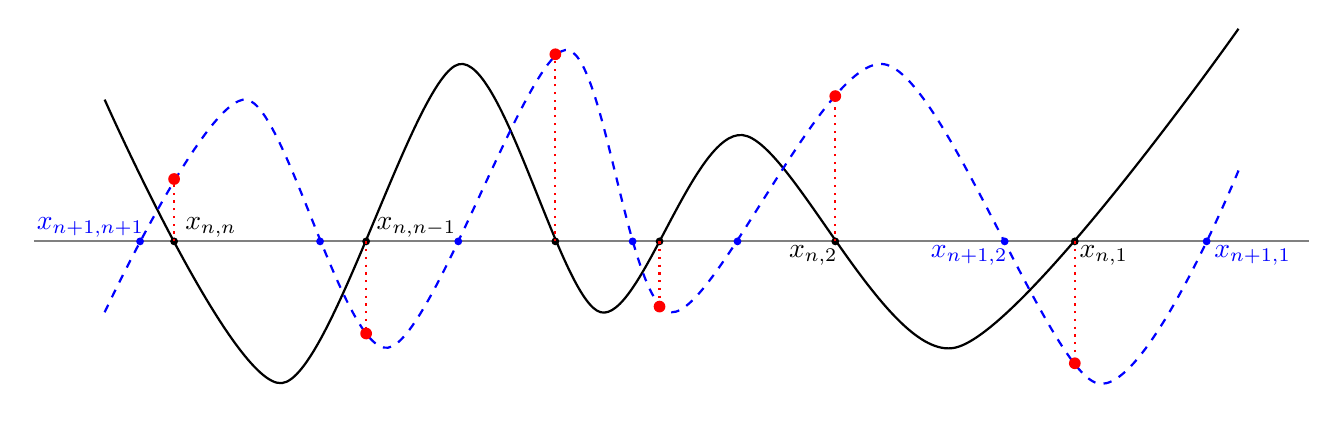
\begin{tikzpicture}[thick,scale=0.9]
  \draw[gray] (-2,0) -- (16,0);
  \draw [black] plot [smooth] coordinates {(-1,2) (1.5,-2) (4,2.5) (6,-1) (8,1.5) (11,-1.5) (15,3)};
  \draw [blue, dashed] plot [smooth] coordinates {(-1,-1) (1,2) (3,-1.5) (5.5,2.7) (7,-1) (10,2.5) (13,-2) (15,1)};
  \node [blue] at (-1.2,.2) {\( x_{n+1,n+1} \)};
  \node [blue] at (15.2,-.2) {\( x_{n+1,1} \)};
  \node [blue] at (11.2,-.2) {\( x_{n+1,2} \)};
  \node at (-.5,0) [blue,circle,fill,inner sep=1pt]{};
  \node at (2.04,0) [blue,circle,fill,inner sep=1pt]{};
  \node at (3.99,0) [blue,circle,fill,inner sep=1pt]{};
  \node at (6.45,0) [blue,circle,fill,inner sep=1pt]{};
  \node at (7.93,0) [blue,circle,fill,inner sep=1pt]{};
  \node at (11.7,0) [blue,circle,fill,inner sep=1pt]{};
  \node at (14.55,0) [blue,circle,fill,inner sep=1pt]{};
  \node at (12.69,0) [circle,fill,inner sep=1pt]{};
  \node at (9.31,0) [circle,fill,inner sep=1pt]{};
  \node at (-.02,0) [circle,fill,inner sep=1pt]{};
  \node at (2.69,0) [circle,fill,inner sep=1pt]{};
  \node at (5.36,0) [circle,fill,inner sep=1pt]{};
  \node at (6.83,0) [circle,fill,inner sep=1pt]{};
  \node at (13.1,-.2) {\( x_{n,1} \)};
  \node at (9.0,-.2) {\( x_{n,2} \)};
  \node at (.5,.2) {\( x_{n,n} \)};
  \node at (3.4,.2) {\( x_{n,n-1} \)};
  \draw [red, dotted] (-.02,0) --++(0,.9);
  \node at (-.02,.88) [red,circle,fill,inner sep=1.5pt]{};
  \draw [red, dotted] (2.69,0) --++(0,-1.3);
  \node at (2.69,-1.3) [red,circle,fill,inner sep=1.5pt]{};
  \draw [red, dotted] (12.69,0) --++(0,-1.72);
  \node at (12.69,-1.72) [red,circle,fill,inner sep=1.5pt]{};
  \draw [red, dotted] (9.31,0) --++(0,2.05);
  \node at (9.31,2.05) [red,circle,fill,inner sep=1.5pt]{};
  \draw [red, dotted] (5.36,0) --++(0,2.64);
  \node at (5.36,2.64) [red,circle,fill,inner sep=1.5pt]{};
  \draw [red, dotted] (6.83,0) --++(0,-0.92);
  \node at (6.83,-0.92) [red,circle,fill,inner sep=1.5pt]{};
\end{tikzpicture}
  \caption{The interchanging zeros of \( P_n(x) \) and \( P_{n+1}(x) \).}
  \label{fig:image2}
\end{figure}
This means that \( P_{n+1}(x) \) has a root between each interval
\( (x_{n,j+1},x_{n,j}) \) for \( j=1,\dots,n-1 \). Considering the
limits \( \lim_{x\to \infty} P_{n+1}(x) = \infty\) and
\( \lim_{x\to -\infty} P_{n+1}(x) = (-1)^{n+1} \infty\), we can see
that \( P_{n+1}(x) \) also has one root in \( (x_{n,1},\infty) \) and
one root in \( (-\infty,x_{n,n}) \). Thus we obtain
\eqref{eq:interlacing}.
\end{proof}

\chapter{Basics of enumerative combinatorics}
\label{cha:basics-enum-comb}

In this chapter we review fundamental objects in enumerative
combinatorics.
From now on we will use the notation \( [n] := \{ 1,\dots,n\} \).

\section{Formal power series and generating functions}

In this section, we study basics of formal power series and generating
functions. See \cite{Wilf2006} for more details on this topic.

A \emph{power series} is a series of the form
\[
 f(x) = a_0 + a_1 x + a_2 x^2 + \cdots.
\]
The quantity \( a_n \) is called the \emph{coefficient of \( x^n \)}
in \( f(x) \). The \emph{constant term} of \( f(x) \) is \( a_0 \),
which we also denote by \( f(0) \).

If the coefficients \( a_n \) are real numbers, then \( f(x) \) may be considered as
a function on \( x \) whose domain is the set of real numbers \( x \)
such that the above infinite series converges. For example, if
\[
  f(x) = 1+x+x^2 + \cdots,
\]
then we have \( f(x) = 1/(1-x) \) for \( |x|<1 \). Thus we can write,
for \( |x|<1 \),
\begin{equation}\label{eq:geometric-series}
  1+x+x^2 + \cdots = \frac{1}{1-x}.
\end{equation}
This, however, does not make sense if \( |x|>1 \). Hence, in calculus,
whenever we consider a power series we always have to mention for what
values of \( x \) the series converges. But in formal power series the
convergence is not needed.

Let \( R \) be a commutative ring with identity. Recall that
\( R[x] \) denotes the ring of polynomials in \( x \) with
coefficients in \( R \).

\begin{defn}
  The \emph{ring of formal power series} in \( x \) with coefficients
  in \( R \) is the set
\[
  R[[x]] = \{a_0 + a_1 x + a_2x^2 + \cdots : a_0,a_1,a_2,\ldots \in R \},
\]
with addition
\[
  \left( \sum_{n=0}^\infty a_n x^n \right) + \left( \sum_{n=0}^\infty
    b_n x^n \right) = \sum_{n=0}^\infty (a_n+b_n) x^n ,
\]
and multiplication
\[
  \left( \sum_{n=0}^\infty a_n x^n \right) \left( \sum_{n=0}^\infty
    b_n x^n \right) = \sum_{n=0}^\infty \left( \sum_{k=0}^n a_k
    b_{n-k} \right)x^n.
\]
\end{defn}

So, roughly speaking, a formal power series is a polynomial of
infinite degree.

The multiplicative identity of \( R[[1]] \) is \( 1 \), that is,
\( 1+0x+0x^2+\cdots \). For \( f(x),g(x) \in R[[1]] \), if
\( f(x) g(x) = 1 \), then we say that \( f(x) \) is the \emph{inverse}
of \( g(x) \) and write \( f(x) = g(x)^{-1} = 1/g(x) \).

In the language of formal power series, \eqref{eq:geometric-series} is
a perfectly valid identity without any convergence considered because
\[
  (1+x+x^2 + \cdots)(1-x) = (1+x+x^2 + \cdots) - x(1+x+x^2 + \cdots) = 1.
\]

An important aspect of formal power series is that the coefficient of
\( x^n \) must be computed using a finitely many additions and
multiplications in \( R \).


\begin{exam}
  The series
\[
  e^{1+x} = \sum_{n\ge 0} \frac{(1+x)^n}{n!}
\]
is not a formal power series in \( \RR[[x]] \) because the constant
term (the coefficient of \( x^0 \)) is \( \sum_{n\ge0} 1/n! \), which
cannot be computed by a finite number of additions and multiplications
in \( \RR \) (although we know \( \sum_{n\ge0} 1/n! = e \)). On the
other hand,
\[
  e\cdot e^{x} = \sum_{n\ge 0} \frac{e x^n}{n!}
\]
is a formal power series in \( \RR[[x]] \). 
\end{exam}

Note that being a formal power series is all about how the series is
presented rather than what values the series take as a function. Most
of the time, we will not consider a formal power series as a function.

For two formal power series \( f(x) = \sum_{n\ge0} f_n x^n \) and
\( g(x) = \sum_{n\ge0} g_n x^n \) with \( g_0=0 \), we define the
\emph{composition} \( (f\circ g)(x) = f(g(x)) \) of \( f(x) \) and
\( g(x) \) by
\begin{equation}\label{eq:12}
  f(g(x)) = \sum_{n\ge0} f_n g(x)^n.
\end{equation}
To see that the above sum is a formal power series, note that since
\( g_0=0 \), every term in \( f_ng(x)^n \) has degree at least
\( n \). Thus, for a fixed \( m\ge0 \), the coefficient of \( x^m \)
in \( f(g(x)) \) is the coefficient of \( x^m \) in the finite sum
\( \sum_{n=0}^m f_n g(x)^n \) of formal power series, which in turn
can be computed in a finite number of additions and multiplications in
\( R \). Note also that if \( g_0\ne 0 \), then the constant term in
the sum \eqref{eq:12} is an infinite sum \( \sum_{n\ge0} f_n g_0 \),
hence \( f(g(x)) \) is not a formal power series (unless \( f(x) \) is
a polynomial).

There is a simple criterion for the existence of an inverse of a
formal power series.

\begin{prop}
  Let \( R \) be a field. A formal power series \( f(x)\in R[[x]] \)
  has an inverse if and only if \( f(0)\ne 0 \).
\end{prop}
\begin{proof}
  (\(\Rightarrow\)) Let \( g(x) \) be the inverse of \( f(x) \).
  Suppose that \( f(0)=0 \). Then the constant term of \( f(x)g(x) \)
  is \( f(0)g(0)=0 \), which is a contradiction to \( f(x)g(x) = 1 \).
  Thus we have \( f(0)\ne 0 \).

  (\(\Leftarrow\)) Let \( f(x) = \sum_{n\ge 0} f_nx^n \).
  Then we can write \( f(x) \) as
  \[
    f(x) = f_0 \left( 1 - h(x) \right),
    \qquad h(x) = \sum_{n\ge 1} h_n x^n, \qquad h_n = - f_0^{-1}f_n.
  \]
  Then the inverse of \( f(x) \) can be found in this way:
  \[
    \frac{1}{f(x)} = \frac{1}{f_0} \cdot \frac{1}{1-h(x)}
    = \frac{1}{f_0} \sum_{n\ge0} h(x)^n.
  \]
  Since the lowest degree term of \( h(x)^n \) has degree at least \( n \),
  the above infinite sum is a well-defined formal power series.
\end{proof}

As in calculus we define the \emph{derivative} of a formal power
series \( f(x) = \sum_{n\ge0} f_n x^n \) by
\[
  f'(x) := \sum_{n\ge1} n f_n x^{n-1} = \sum_{n\ge0} (n+1) f_{n+1} x^{n}.
\]
The usual differentiation rules hold.
\begin{prop}
  For two formal power series \( f(x) \) and \( g(x) \),
  we have
\begin{align*}
  (f(x)g(x))'
  &= f'(x) g(x) + f(x) g'(x), \\
  \left(\frac{f(x)}{g(x)}\right)'
  &= \frac{f'(x) g(x) - f(x) g'(x)}{g(x)^2}, \qquad g(x) \ne 0,\\
  (f(g(x)))'
  &= f'(g(x)) g'(x), \qquad g(0) = 0.
\end{align*}
\end{prop}

\begin{proof}
  We can prove these identities using the formal definition of the
  derivative. We will only proof the first identity. Let
  \( f(x) = \sum_{n\ge0} f_n x^n \) and
  \( g(x) = \sum_{n\ge0} g_n x^n \). Then
  \[
    (f(x)g(x))' = \left( \sum_{n\ge 0} \left( \sum_{k=0}^{n} f_kg_{n-k} \right) x^{n} \right)'
      = \sum_{n\ge 0} \left( \sum_{k=0}^{n} n f_kg_{n-k}
    \right) x^{n-1}.
  \]
  On the other hand,
  \begin{align*}
    f'(x) g(x) + f(x) g'(x)
    & =  \sum_{n\ge0} n f_n x^{n-1} \sum_{n\ge0} g_n x^n +   
      \sum_{n\ge0} f_n x^n \sum_{n\ge0} n g_n x^{n-1}\\
    &= \sum_{n\ge 0} \left( \sum_{k=0}^{n} kf_kg_{n-k}
      + \sum_{k=0}^{n} f_k\cdot (n-k)g_{n-k} \right) x^{n-1}\\
    &= \sum_{n\ge 0} \left( \sum_{k=0}^{n} nf_kg_{n-k} \right) x^{n-1}.
  \end{align*}
  Thus we get the first identity.
\end{proof}





We can naturally extend the definition of formal power series to the
multivariate case.


\begin{defn}
  Let \( \vx =(x_1,x_2,\dots) \) be a sequence of variables. Let
  \( Z \) denote the set of sequences
  \( I=(i_1,i_2,\dots)\in \ZZ_{\ge0}^\infty \) such that
  \( i_1+i_2 + \cdots < \infty \). For \( I=(i_1,i_2,\dots)\in Z \),
  we write \( \vx^I = x_1^{i_1} x_2^{i_2} \cdots \). The \emph{ring of
    formal power series} in \( x_1,x_2,\dots \) with coefficients in
  \( R \) is the set
\[
  R[[\vx]] = \left\{ \sum_{I\in Z} a_I \vx^I  : a_I\in R \right\},
\]
with addition
\[
  \left(\sum_{I\in Z} a_I \vx^I \right) + \left(\sum_{I\in Z} b_I \vx^I
  \right) = \left( \sum_{I\in Z} (a_I+b_I) \vx^I \right),
\]
and multiplication
\[
  \left(\sum_{I\in Z} a_I \vx^I \right) \left(\sum_{I\in Z} b_I \vx^I
  \right) = \sum_{I\in Z} \left( \sum_{I_1,I_2\in Z, I_1+I_2=I} a_{I_1} b_{I_2} \right) \vx^I.
\]
\end{defn}

Again, rougly speaking, a multivariate formal power series is a
multivariate polynomial of infinite degree.


Now we define the notion of generating functions.


\begin{defn}
  The \emph{generating function} for a sequences \( \{ a_n\}_{n\ge 0} \) is
  defined to be the formal power series
\[
  a_0 + a_1 x + a_2 x^2 + \cdots.
\]
\end{defn}

So, the generating function for \( \{ a_n\}_{n\ge 0} \) is nothing but
a way of recording the sequence. One of the benefits of generating
functions is that we can use many properties of formal power series.


\begin{exam}
  The generating function for \( \{ a_n = 2^n\}_{n\ge 0} \) is
  \begin{equation}\label{eq:15}
    \sum_{n\ge 0} 2^n x^n = \sum_{n\ge 0} (2x)^n = \frac{1}{1-2x}.
  \end{equation}
\end{exam}

\begin{exam}
  Let's find the generating function for \( \{ a_n = n 2^n\}_{n\ge 0} \).
  Differentiating both sides of \eqref{eq:15}, we get
  \[
    \sum_{n\ge 0} n2^n x^{n-1} =  \frac{2}{(1-2x)^2}.
  \]
  Multiplying both sides by \( x \), we obtain
  \[
    \sum_{n\ge 0} n2^n x^{n} =  \frac{2x}{(1-2x)^2}.
  \]
\end{exam}

We can easily extend the definition of generating functions to
accommodate arrays \( \{ a_I\}_{I\in Z} \) of elements \( a_I\in R \)
using multivariate formal power series. More generally, we will
consider generating functions for arbitrary (combinatorial) objects.

\begin{defn}
  Let \( A \) be a set of objects. A \emph{weight} on \( A \) is a
  function \( \wt:A\to R \), where \( R \) is any commutative ring.
  The \emph{generating function} for \( A \) with respect to the
  weight function \( \wt \) is the formal power series
  \[
    \sum_{a \in A} \wt(a).
  \]
\end{defn}



\begin{exam}
  Let \( A = \{0,1,2,\dots\} \) and define a weight of \( A \) by
  \( \wt(a) = x^a \). Then the generating function for \( A \)
  (with this weight) is
  \[
    \sum_{a \in A} \wt(a) = \sum_{n=0}^n \wt(n)
    = \sum_{n=0}^n x^n = \frac{1}{1-x}.
  \]
\end{exam}

\begin{exam}
  Let \( A \) be the set of subsets of \( [n] \) and define a weight
  of \( A \) by \( \wt(a) = x^{|a|}y^{n-|a|} \). Then the generating function for
  \( A \) (with this weight) is
  \[
    \sum_{a \in A} \wt(a) = \sum_{a\subseteq [n]} x^{|a|} y^{n-|a|} =
    \sum_{k=0}^n \binom{n}{k} x^{k}y^{n-k} = (x+y)^n.
  \]
\end{exam}

\begin{exam}
  Let \( A \) be the set \( S_n \) of permutations of \( [n] \) and
  define a weight of \( A \) by \( \wt(a) = x^{\cycle(a)} \). Then it
  can be proved (see \eqref{eq:c(n,k)-gf}) that the generating
  function for \( A \) (with this weight) is
  \[
    \sum_{a \in A} \wt(a) = \sum_{\pi\in S_n} x^{\cycle(a)} = x(x+1)
    \cdots (x+n-1).
  \]
\end{exam}

We will often use the term ``generating function'' in a flexible
manner. For example, the generating function for the number of
permutations would mean the generating function for the sequence
\( \{a_n = n!\}_{n\ge0} \), that is, \( \sum_{n\ge0} n! x^n \).

\section{Dyck paths and Motzkin paths}

In this section we introduce two important classes of lattice paths.
These are fundamental objects in studying orthogonal polynomials
combinatorially.


\begin{defn}
  A \emph{lattice path} from \( u \) to \( v \) is a sequence
  \( \pi = (v_0,v_1,\dots,v_n) \) of points in \( \ZZ\times\ZZ \) with
  \( v_0=u \) and \( v_n =v \). Each pair \( (v_i,v_{i+1}) \) of
  consequence points is called a \emph{step} of \( \pi \). 
\end{defn}

A path \( \pi = (v_0,v_1,\dots,v_n) \) is also considerd as a sequence
\( S_1 \cdots S_n \) of steps, where \( S_i=(v_{i-1},v_i) \). We will
sometimes identify a step \( (v_i,v_{i+1}) \) with
\( v_{i+1} - v_i \in \ZZ\times\ZZ \).

\begin{defn}
  A \emph{Dyck path} is a lattice path consisting of \emph{up steps}
  \( (1,1) \) and \emph{down steps} \( (1,-1) \) that stays on or
  above the \( x \)-axis, see \Cref{fig:dyck-path}. Denote by
  \( \Dyck(u\to v) \) the set of Dyck paths from \( u \) to \( v \).
  We also define \( \Dyck_{2n} = \Dyck((0,0)\to (2n,0))\).
\end{defn}

\begin{figure}
  \centering
  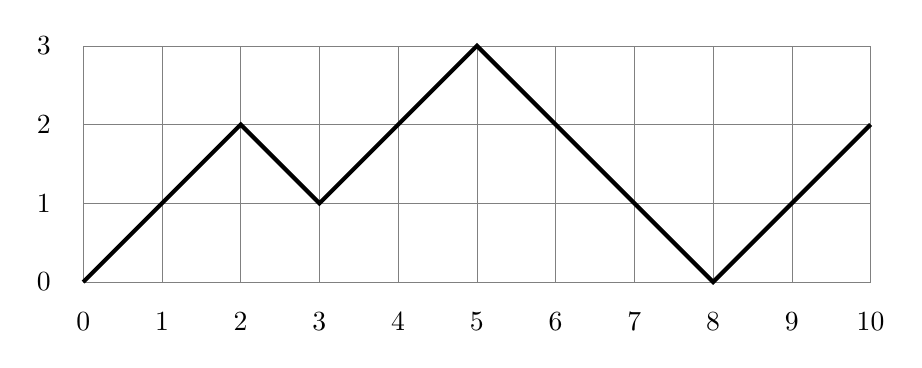
\begin{tikzpicture}
      \draw[help lines] (0,0) grid (10,3);
\foreach \x in {0,...,10} \draw node at (\x,-.5) {\( \x \)};
\foreach \y in {0,...,3} \draw node at (-.5,\y) {\( \y \)};
\draw[line width = 1.5pt] (0,0) -- ++(1,1) -- ++(1,1) -- ++(1,-1) -- ++(1,1) -- ++(1,1) -- ++(1,-1) -- ++(1,-1) -- ++(1,-1) -- ++(1,1) -- ++(1,1);
  \end{tikzpicture}
  \caption{A Dyck path from \( (0,0) \) to \( (10,2) \).}
  \label{fig:dyck-path}
\end{figure}



Let's enumerate the Dyck paths in \( \Dyck_{2n} \) using generating
functions. To do this let
\[
  C(x) = \sum_{n\ge 0} |\Dyck_{2n}| x^n.
\]
Then
we can also write
\[
  C(x) = \sum_{\pi\in \Dyck} \wt(\pi),
\]
where \( \Dyck \) is the set of all Dyck paths from \( (0,0) \) to
\( (2n,0) \) for some \( n\ge0 \) and \( \wt(\pi) = x^{d(\pi)} \),
where \( d(\pi) \) is the number of down steps in \( \pi \). It is
helpful to imagine the generating function \( C(x) \) as a picture of
all Dyck paths, where each Dyck path has its weight attached to it as
shown in \Cref{fig:gf-dyck}.

\begin{figure}
  \centering
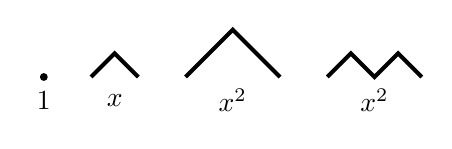
\begin{tikzpicture}[scale=0.3]
\node at (0,0) [circle,fill,inner sep=1pt]{};
\draw[line width = 1.5pt] (2,0) -- ++(1,1) -- ++(1,-1);
\draw[line width = 1.5pt] (6,0) -- ++(1,1) -- ++(1,1) -- ++(1,-1) -- ++(1,-1);
\draw[line width = 1.5pt] (12,0) -- ++(1,1) -- ++(1,-1) -- ++(1,1) -- ++(1,-1);
\node at (0,-1) {\( 1 \)};
\node at (3,-1) {\( x \)};
\node at (8,-1) {\( x^2 \)};
\node at (14,-1) {\( x^2 \)};
\end{tikzpicture}
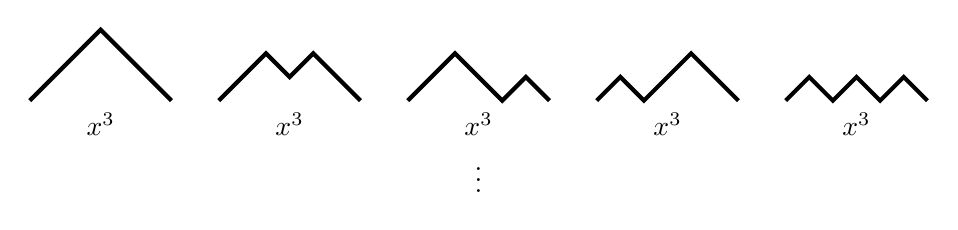
\begin{tikzpicture}[scale=0.3]
\draw[line width = 1.5pt] (0,0) -- ++(1,1) -- ++(1,1) -- ++(1,1) -- ++(1,-1) -- ++(1,-1) -- ++(1,-1);
\draw[line width = 1.5pt] (8,0) -- ++(1,1) -- ++(1,1) -- ++(1,-1) -- ++(1,1) -- ++(1,-1) -- ++(1,-1);
\draw[line width = 1.5pt] (16,0) -- ++(1,1) -- ++(1,1) -- ++(1,-1) -- ++(1,-1) -- ++(1,1) -- ++(1,-1);
\draw[line width = 1.5pt] (24,0) -- ++(1,1) -- ++(1,-1) -- ++(1,1) -- ++(1,1) -- ++(1,-1) -- ++(1,-1);
\draw[line width = 1.5pt] (32,0) -- ++(1,1) -- ++(1,-1) -- ++(1,1) -- ++(1,-1) -- ++(1,1) -- ++(1,-1);
\node at (3,-1) {\( x^3 \)};
\node at (11,-1) {\( x^3 \)};
\node at (19,-1) {\( x^3 \)};
\node at (27,-1) {\( x^3 \)};
\node at (35,-1) {\( x^3 \)};
\node at (19,-3) {\( \vdots \)};
\end{tikzpicture}
  \caption{An illustration of the generating function for Dyck paths.}
  \label{fig:gf-dyck}
\end{figure}


\begin{figure}
  \centering
  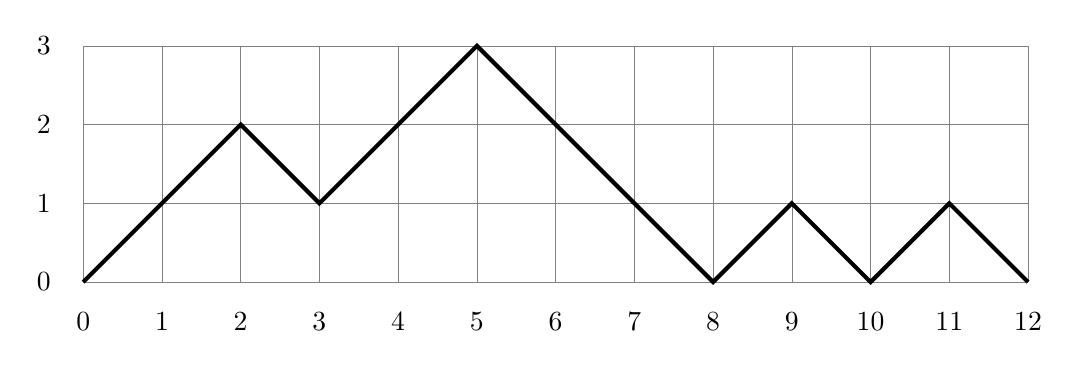
\begin{tikzpicture}
    \draw[help lines] (0,0) grid (12,3);
\foreach \x in {0,...,12} \draw node at (\x,-.5) {\( \x \)};
\foreach \y in {0,...,3} \draw node at (-.5,\y) {\( \y \)};
\draw[line width = 1.5pt] (0,0) -- ++(1,1) -- ++(1,1) -- ++(1,-1) -- ++(1,1) -- ++(1,1) -- ++(1,-1) -- ++(1,-1) -- ++(1,-1) -- ++(1,1) -- ++(1,-1) -- ++(1,1) -- ++(1,-1);
  \end{tikzpicture}
  \caption{A Dyck path \( \pi \) from \( (0,0) \) to \( (12,0) \).}
  \label{fig:dyck-path2}
\end{figure}

A Dyck path \( \pi \in \Dyck \) can be considered as a sequence of up
steps and down steps. For example, the Dyck path in
\Cref{fig:dyck-path2} is \( \pi = UUDUUDDDUDUD \). Every nonempty Dyck
path \( \pi \in \Dyck \) is uniquely decomposed into
\( \pi = U \tau D \rho \) for some \( \tau,\rho\in \Dyck \). For our
running example,
\begin{equation}\label{eq:dyck-decomp}
  \pi=UUDUUDDDUDUD = U(UDUUDDD)(UDUD),
\end{equation}
so we have
\( \tau = UDUUDDD \) and \( \rho = UDUD \).
This argument shows that
\begin{equation}\label{eq:cat-gf}
  C(x) = 1 + C(x) x C(x).
\end{equation}
Solving this quadratic equation for \( C(x) \), we
get
\begin{equation}\label{eq:16}
   C(x)  = \frac{1\pm\sqrt{1-4x}}{2x}.
  \end{equation}

  We must choose the correct sign here. First, by setting \( x=0 \),
  we obtain that the constant term of \( \sqrt{1-4x} \) is \( 1 \).
  Thus \eqref{eq:16} is a valid formal power series only for the minus
  sign. This implies that
  \[
    \sum_{n\ge0} |\Dyck_{2n}| x^n = \frac{1-\sqrt{1-4x}}{2x}.
  \]
 
  Now we can use the \emph{binomial theorem}
\[
  (1+x)^\alpha := \sum_{n\ge 0} \binom{\alpha}{n} x^n,
\]
where
\[
  \binom{\alpha}{n} = \frac{\alpha(\alpha-1)\cdots (\alpha-n+1)}{n!}.
\]
By the binomial theorem, we have
  \begin{align*}
    \sqrt{1-4x}
    &= (1-4x)^{1/2} = \sum_{n\ge 0} \binom{1/2}{n} (-4x)^n
    = 1+ \sum_{n\ge 1} \frac{\frac{1}{2} \frac{-1}{2}
    \frac{-3}{2} \cdots \frac{-2n+3}{2}}{n!} (-1)^n 4^n x^n\\
    &= 1- \sum_{n\ge 1} \frac{1\cdot 3\cdot \cdots \cdot (2n-3)}{n!} 2^n x^n
    = 1- \sum_{n\ge 1} \frac{2(2n-2)!}{n!(n-1)!} x^n .
  \end{align*}
  Therefore,
  \[
   \sum_{n\ge0} |\Dyck_{2n}| x^n = \frac{1-\sqrt{1-4x}}{2x} 
   = \sum_{n\ge 1} \frac{1}{n} \binom{2n-2}{n-1} x^{n-1}
   = \sum_{n\ge 0} \frac{1}{n+1} \binom{2n}{n} x^n.
  \]
  Comparing the coefficient of \( x^n \) in both sides we obtain the
  following result.

\begin{prop}
  We have
  \begin{equation}\label{eq:17}
    |\Dyck_{2n}| = \frac{1}{n+1} \binom{2n}{n}.
  \end{equation}
\end{prop}
Note that we proved \eqref{eq:17} using generating functions, but this
can also be proved by a standard reflection principle.

The \emph{Catalan number} \( C_n \) is defined by
\[
  C_n = \frac{1}{n+1} \binom{2n}{n}.
\]
The first few Catalan numbers are
\[
  1, 1, 2, 5, 14, 42, 132, 429, 1430, 4862, \ldots.
\]

There are many combinatorial objects counted by the Catalan number.
Stanley \cite{Stanley2015} collected more than 200 such ``Catalan
objects''. Dyck paths are one of the most well-known Catalan objects.
Some of other well known Catalan objects are triangulations of an
\( (n+2) \)-gon, ballot sequences of length \( 2n \), and plane binary
trees with \( n \) vertices.

The Catalan numbers satisfy the following recurrence:
\begin{equation}\label{eq:cat-rec}
  C_0 = 1, \qquad
  C_n = \sum_{k=0}^{n} C_k C_{n-1-k}, \qquad n\ge1.
\end{equation}
This recurrence can be proved similarly as \eqref{eq:cat-gf} using the
decomposition \eqref{eq:dyck-decomp}.


Now we consider lattice paths with three kinds of steps. These lattice
paths will play a fundamental role in Viennot's theory of orthogonal
polynomials.

\begin{defn}
  A \emph{Motzkin path} is a lattice path consisting of \emph{up
    steps} \( (1,1) \), \emph{horizontal steps} \( (1,0) \), and
  \emph{down steps} \( (1,-1) \) that stays on or above the
  \( x \)-axis, see Figure~\ref{fig:motzkin}. Denote by
  \( \Motz(u\to v) \) the set of Dyck paths from \( u \) to \( v \).
  We also define \( \Motz_{n} = \Motz((0,0)\to (n,0))\).
\end{defn}

\begin{figure}
  \centering
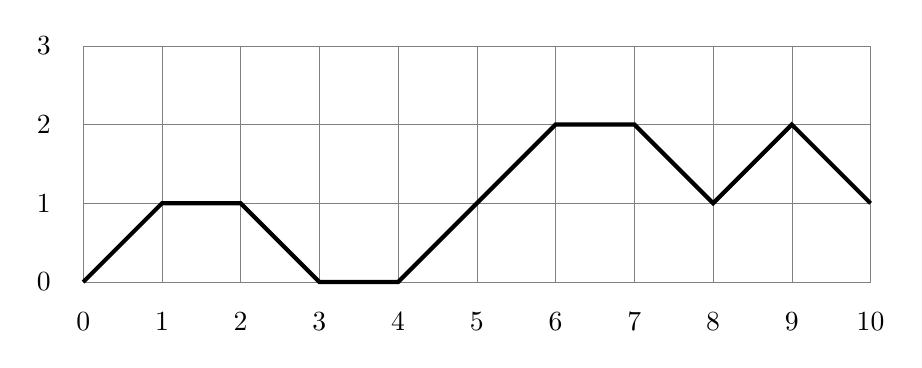
\begin{tikzpicture}
  \draw[help lines] (0,0) grid (10,3);
\foreach \x in {0,...,10} \draw node at (\x,-.5) {\( \x \)};
\foreach \y in {0,...,3} \draw node at (-.5,\y) {\( \y \)};
\draw[line width = 1.5pt] (0,0) -- ++(1,1) -- ++(1,0) -- ++(1,-1) -- ++(1,0) -- ++(1,1) -- ++(1,1) -- ++(1,0) -- ++(1,-1) -- ++(1,1) -- ++(1,-1);
\end{tikzpicture}
\caption{A Motzkin path from \( (0,0) \) to \( (10,1) \).}
  \label{fig:motzkin}
\end{figure}

Considering the positions of horizontal steps, we can relate the
number of Motzkin paths and that of Dyck paths.



\begin{prop}
  We have
  \[
    |\Motz_{n}| = \sum_{k=0}^{\flr{n/2}} \binom{n}{2k} C_k.
  \]
\end{prop}

\begin{prop}
  Let \( M(x) = \sum_{n\ge 0} |\Motz_n| x^n \). Then
  \[
    M(x) = \frac{1-x-\sqrt{1-2x-3x^2}}{2x^2}.
  \]
\end{prop}
\begin{proof}
  By a similar argument used to prove  \eqref{eq:cat-gf},
  we have
  \[
    M(x) = 1 + x M(x) + M(x) x^2 M(x).
  \]
  Solving the equation we obtain the desired formula.
\end{proof}


\section{Set partitions and matchings}

In this section we study set partitions and matchings. They will be
used to give combinatorial interpretations for moments of Charilier
polynomials and Hermite polynomials.

\begin{defn}
  A \emph{set partition} of a set \( X \) is a collection
  \( \pi = \{B_1,\dots,B_k\} \) of subsets of \( X \)
  such that
  \begin{enumerate}
  \item \( B_i\ne\emptyset \) for all \( i \),
  \item \( B_i\cap B_j = \emptyset \) for all \( i\ne j \), and
  \item \( B_1 \cup \cdots \cup B_k = X \).
  \end{enumerate}
  Each \( B_i \) is called a \emph{block} of \( \pi \).
\end{defn}

A set partition can be visualized by connecting consecutive elements
in each block see \Cref{fig:set-partition}.

\begin{figure}
  \centering
  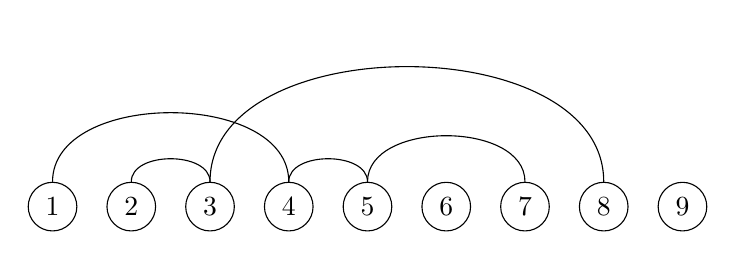
\begin{tikzpicture}
    \begin{scope}[shift={(0,0)}]
\node[draw, circle] (1) at (1,0) {\( 1 \)};
\node[draw, circle] (4) at (4,0) {\( 4 \)};
\node[draw, circle] (5) at (5,0) {\( 5 \)};
\node[draw, circle] (7) at (7,0) {\( 7 \)};
\draw[out=90,in=90] (1) to (4);
\draw[out=90,in=90] (4) to (5);
\draw[out=90,in=90] (5) to (7);
\node[draw, circle] (2) at (2,0) {\( 2 \)};
\node[draw, circle] (3) at (3,0) {\( 3 \)};
\node[draw, circle] (8) at (8,0) {\( 8 \)};
\draw[out=90,in=90] (2) to (3);
\draw[out=90,in=90] (3) to (8);
\node[draw, circle] (6) at (6,0) {\( 6 \)};
\node[draw, circle] (9) at (9,0) {\( 9 \)};
\end{scope}
\end{tikzpicture}
\caption{A visualization of a set partition
  \( \{\{1,4,5,7\}, \{2,3,8\}, \{6\}, \{9\}\} \) of \( [9] \).}
\label{fig:set-partition}
\end{figure}

We denote by \( \Pi_n \) the set of all set partitions of \( [n] \).
We also define \( \Pi_{n,k} \) to be the set of all set partitions of
\( [n] \) with exactly \( k \) blocks. The \emph{Stirling number of
  the second kind} \( S(n,k) \) is the cardinality of \( \Pi_{n,k} \).

We use the convention that \( \emptyset \) is the only set partition
of \( \emptyset \), i.e., \( \Pi_0 = \{\emptyset\} \). The following
are immediate from the definition of set partitions:
\begin{itemize}
\item \( S(n,0) = \delta_{n,0} \),
\item \( S(n,n) = 1 \),
\item \( S(n,k) = 0 \) if \( k>n \).
\end{itemize}

We can compute the number \( S(n,k) \) using the following recursion
with the above initial conditions.

\begin{prop}
  For integers \( n,k\ge1 \), we have
  \[
    S(n,k) = S(n-1,k-1) + k S(n-1,k).
  \]
\end{prop}
\begin{proof}
  Let \( \pi\in \Pi_{n,k} \). If \( n \) is in a singleton of
  \( \pi \), then \( \pi\setminus\{n\} \in \Pi_{n-1,k-1} \). Otherwise,
  \( \pi \) can be obtained from a set partition
  \( \pi'\in \Pi_{n-1,k} \) by adding \( n \) to one of the \( k \)
  blocks of \( \pi' \). This shows the recursion.
\end{proof}


\begin{prop}
  We have
  \[
    S(n,k) = \frac{1}{k!} \sum_{i=0}^{k} (-1)^{k-i} \binom{k}{i}i^n.
  \]
\end{prop}

\begin{proof}
  The number of onto functions \( f:[n] \to [k] \) is \( k! S(n,k) \).
  By the principle of inclusion and exclusion, this number is equal to
  \[
     k! S(n,k) = \sum_{i=0}^{k} (-1)^{k-i} \binom{k}{i}i^n,
  \]
  which implies the desired formula.
\end{proof}

For an integer \( n\ge0 \), a \emph{falling factorial} \( (x)_n \) is defined by
\[
  (x)_n = x(x-1) \cdots (x-n+1).
\]

\begin{prop}
  We have
  \begin{equation}\label{eq:S(n,k)(x)k=xn}
    \sum_{k=0}^{n} S(n,k) (x)_k = x^n.
  \end{equation}
\end{prop}

\begin{proof}
  Since both sides are polynomials in \( x \), it suffices to show
  that the identity holds for all positive integers \( x \). So, let's
  assume that \( x \) is a positive integer. Then the right-hand side
  is the number of all functions \( f: [n] \to [x] \).

  Now, consider a function \( f: [n] \to [x] \) such that the image
  \( f([n]) \) has exactly \( k \) elements. Let
  \( f([n]) = \{a_1<\dots<a_k\} \). Then
  \( \{f^{-1}(a_1),\dots,f^{-1}(a_k)\} \) is a set partition of
  \( [n] \) with \( k \) blocks. Thus such a function \( f \) is
  obtained by first partitionining \( [n] \) into \( k \) blocks
  \( B_1,\dots,B_k \) and constructing a one-to-one map from
  \( \{B_1,\dots,B_k\} \) to \( [x] \). This shows that the number of
  such functions is \( S(n,k) (x)_k \). Summing over all \( k \) gives
  the number of all functions \( f: [n] \to [x] \).

  Since both sides of the identity count the same number, they are
  equal.
\end{proof}

\begin{defn}
  A \emph{matching} on a set \( X \) is a set partition
  \( \pi = \{B_1,\dots,B_k\} \) of \( X \) in which every block has
  size \( 1 \) or \( 2 \). Each block of size \( 1 \) is called a
  \emph{fixed point} and each block of size \( 2 \) is called an
  \emph{edge} or an \emph{arc} of \( \pi \).
\end{defn}

A matching is said to be \emph{perfect} or \emph{complete} if there
are no fixed points.

\begin{prop}
  The number of complete matchings of \( [2n] \) is
  \[
    (2n-1)!! := 1 \cdot 3 \cdot \cdots \cdot (2n-1).
  \]
  The number of matchings of \( [n] \) is
  \[
    \sum_{k=0}^{\flr{n/2}} \binom{n}{2k} (2k-1)!!.
  \]
\end{prop}

\begin{proof}
  The first identity can easily be proved by induction on \( n \)
  since there are \( 2n-1 \) ways to form an edge with the last
  element \( 2n \) and another element.

  The second identity follows from the observation that if a matching
  of \( [n] \) has \( k \) edges, then these edges form a complete
  matching on a set of size \( 2k \).
\end{proof}

\section{Permutations}

In this section we study permutations, which are one of the most
fundamental objects in combinatorics. We will see later a connection
between permutations and moments of Laguerre polynomials.

\begin{defn}
  A \emph{permutation} on \( [n] \) is a bijection
  \( \pi:[n] \to [n] \). The \emph{symmetric group} \( \sym_n \) is
  the group of permutations on \( [n] \) with multiplication given by
  composition of functions.
\end{defn}

For \( \pi,\tau\in \sym_n \), we write \( \pi\tau = \pi\circ \tau \),
that is \( \pi\tau \) is the permutation defined by
\( (\pi\tau)(i) = \pi(\tau(i)) \).

Let \( \pi:[n] \to [n] \) be a permutation. We will often write
\( \pi_i = \pi(i) \) and identify this permutation with a word
\[
  \pi = \pi_1\pi_2 \cdots \pi_n,
\]
which is called the \emph{one-line notation} of \( \pi \). The
\emph{two-line notation} of \( \pi \) is the array
\[
\pi = \begin{pmatrix}
1 & 2 & \cdots & n\\
\pi_1 & \pi_2 & \cdots & \pi_n
\end{pmatrix}.
\]

\begin{exam}
  Let \( \pi\in\sym_3 \) be the permutation given by
  \[
    \pi(1) = 2, \pi(2) = 3, \pi(3) =1.
  \]
  Then in one-line notation,
  \[
    \pi = \pi_1\pi_2\pi_3 = 2 3 1
  \]
  and in two-line notation,
  \[
    \pi =
    \begin{pmatrix}
1 & 2 & 3\\
2 & 3 & 1
\end{pmatrix}.
  \]
  We have
  \[
    \pi^2 =
    \begin{pmatrix}
1 & 2 & 3\\
3 & 1 & 2
    \end{pmatrix}, \qquad
        \pi^3 =
    \begin{pmatrix}
1 & 2 & 3\\
1 & 2 & 3
    \end{pmatrix}.
  \]
\end{exam}


A \emph{cycle} of \( \pi \) is a sequence \( (a_1,\dots,a_k) \) of
distinct elements of \( [n] \) such that
\[
  \pi(a_1) = a_2, \qquad  
  \pi(a_2) = a_3, \qquad 
  \ldots, \qquad 
  \pi(a_k) = a_1.
\]
We denote by \( \cycle(\pi) \) the number of cycles in \( \pi \).

A cycle \( (a_1,\dots,a_k) \) is considered to be the same as any of
its \emph{cyclic shift} \( (a_j,\dots, a_k, a_1, \dots,a_{j-1}) \). We
also consider a cycle \( \rho=(a_1,\dots,a_k) \) as a permutation of
\( [n] \) such that
\[
  \rho(i) =
  \begin{cases}
   i & \mbox{if \( i\not\in \{a_1,\dots,a_k\} \)},\\
    a_{j+1} & \mbox{if \( i=a_j \),}
  \end{cases}
\]
where \( a_{k+1} = a_1 \).

A \emph{cycle of length \( k \)} is a permutation (in some
\( \sym_n \)) of the form \( (a_1,\dots,a_k) \). A
\emph{transposition} is a cycle of length \( 2 \). A \emph{simple
  transposition} is a transposition of the form \( (i,i+1) \).

Note that for a permutation \( \pi = \pi_1 \cdots \pi_n \in \sym_n \)
and a transposition \( \tau = (i,j)\in \sym_n \) with \( i<j \), the
product \( \pi\tau \) is the permutation obtained from \( \pi \)
by interchaning the values \( \pi_i \) and \( \pi_j \) at the
positions \( i \) and \( j \):
\[
  \pi\tau = \pi_1 \cdots \pi_{i-1} \pi_j \pi_{i+1} \cdots \pi_{j-1}
  \pi_i \pi_{j+1} \cdots \pi_n.
\]
On the other hand, the product \( \tau\pi \) is the permutation
obtained from \( \pi \) by interchaning the values \( i \) and
\( j \). For example, if \( \pi = \cdots i \cdots j \cdots \), then
\( \tau\pi = \cdots j \cdots i \cdots \).


\begin{prop}\label{pro:cycle-decomp}
  Let \( \pi \in \sym_n \). Then we can write
  \( \pi = \rho_1 \cdots \rho_k \) for some disjoint cycles
  \( \rho_1,\dots,\rho_k \) in \( \sym_n \). Moreover, we can also
  write \( \pi = s_1 \cdots s_r \) for some (not necessarily disjoint)
  simple transpositions \( s_i\in \sym_n \).
\end{prop}
\begin{proof}
  Let \( \pi\in \sym_n \). Let \( m=1 \) and consider the sequence
  \( \pi(m), \pi^2(m), \ldots \). Since this is an infinite sequence
  of integers in \( [n] \), we must have \( \pi^i(m) = \pi^j(m) \) for
  some \( i<j \). By multiplying \( \pi^{-i} \), we have
  \( m = \pi^{j-i}(m) \). Thus we can find the smallest integer
  \( r \) such that \( \pi^r(m) = m \). Let \( \rho_1 \) be the cycle
  \( (k,\pi(k), \pi^2(k),\dots,\pi^{r-1}(k)) \).

  Now let \( m \) be the smallest integer in \( [n] \) except those in
  \( \rho_1 \). We repeat this process and obtain cycles
  \( \rho_1,\dots,\rho_k \) whose union as a set is \( [n] \). These
  cycles are disjoint because if \( \rho_i \) and \( \rho_j \) have a
  common element then they must be the same cycle.

  For the second statement, let \( \pi=\pi_1 \cdots \pi_n \). Note
  that multiplying a simple transposition \( (i,i+1) \) on the left of
  \( \pi \) interchanges \( \pi_i \) and \( \pi_{i+1} \). Thus we can
  sort \( \pi=\pi_1 \cdots \pi_n \) into the the identity permutation
  \( 1 2 \cdots n \) by multiplying simple transpositions
  \( t_1, \ldots, t_r \) on the left, i.e.,
  \( \pi t_1 \cdots t_r = id \). Then \( \pi = t_r \cdots t_1 \),
  which is a product of simple transpositions.
\end{proof}


By \Cref{pro:cycle-decomp}, we can write \( \pi \) in \emph{cycle
  notation}, i.e., as a product of its disjoint cycles:
\[
  \pi = \rho_1 \cdots \rho_r.
\]

\begin{exam}
  Let \( \pi = 951826743 \in \sym_9 \).
  In two-line notation,
  \[
    \pi =
\begin{pmatrix}
1 & 2 & 3 & 4 & 5 & 6 & 7 & 8 & 9\\
9 & 5 & 1 & 8 & 2 & 6 & 7 & 4 & 3
\end{pmatrix}.
  \]
  There are 5 disjoint cycles of \( \pi \), namely, \( (1,9,3) \),
  \( (2,5) \), \( (4,8) \), \( (6) \), and \( (7) \). Thus, in cycle
  notation,
  \[
    \pi = (1,9,3)(2,5)(4,8) (6) (7).
  \]
  Thus, \( \cycle(\pi) = 5 \). We sometime omit the cycles of length
  \( 1 \) and write
  \[
    \pi = (1,9,3)(2,5)(4,8).
  \]
\end{exam}

We can also visualize a permutation by drawing its cycles as shown in
\Cref{fig:cycle}.

\begin{figure}
  \centering
  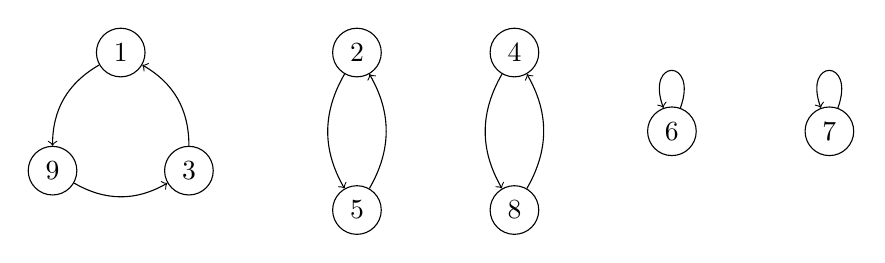
\begin{tikzpicture}
    \begin{scope}[shift={(0,0)}]
\node[draw, circle] (0) at ({90 + (360/3 * 0)}:1) {\( 1 \)};
\node[draw, circle] (1) at ({90 + (360/3 * 1)}:1) {\( 9 \)};
\node[draw, circle] (2) at ({90 + (360/3 * 2)}:1) {\( 3 \)};
\draw[->,bend right] (0) to (1);
\draw[->,bend right] (1) to (2);
\draw[->,bend right] (2) to (0);
\end{scope}
\begin{scope}[shift={(3,0)}]
\node[draw, circle] (0) at ({90 + (360/2 * 0)}:1) {\( 2 \)};
\node[draw, circle] (1) at ({90 + (360/2 * 1)}:1) {\( 5 \)};
\draw[->,bend right] (0) to (1);
\draw[->,bend right] (1) to (0);
\end{scope}
\begin{scope}[shift={(5,0)}]
\node[draw, circle] (0) at ({90 + (360/2 * 0)}:1) {\( 4 \)};
\node[draw, circle] (1) at ({90 + (360/2 * 1)}:1) {\( 8 \)};
\draw[->,bend right] (0) to (1);
\draw[->,bend right] (1) to (0);
\end{scope}
\begin{scope}[shift={(7,-1)}]
\node[draw, circle] (0) at ({90 + (360/1 * 0)}:1) {\( 6 \)};
\draw[->,out=70,in=110,looseness=8] (0) to (0);
\end{scope}
\begin{scope}[shift={(9,-1)}]
\node[draw, circle] (0) at ({90 + (360/1 * 0)}:1) {\( 7 \)};
\draw[->,out=70,in=110,looseness=8] (0) to (0);
\end{scope}
  \end{tikzpicture}
  \caption{A visualization of a permutation
    \( \pi = (1,9,3)(2,5)(4,8) (6) (7) \in \sym_9 \).}
  \label{fig:cycle}
\end{figure}


\begin{defn}
  A permutation \( \pi\in \sym_n \) is called an \emph{involution} if
  \( \pi^2 = \iota \), where \( \iota \) is the identity permutation
  on \( [n] \). Let \( \invol_n \) denote the set of involutions in
  \( \sym_n \).
\end{defn}

\begin{prop}
  There is a bijection between \( \invol_n \) and the set of matchings
  on \( [n] \).
\end{prop}

\begin{proof}
  A permutation \( \pi\in \sym_n \) is an involution if and only if
  every cycle is of length \( 1 \) or \( 2 \). Thus, if \( \pi \) is
  an involution, changing each cycle of \( \pi \) into a block gives a
  matching on \( [n] \). This is clearly a bijection.
\end{proof}



\begin{defn}
  An \emph{inversion} of a permutation \( \pi\in \sym_n \) is a pair
  \( (i,j) \) of integers \( 1\le i<j\le n \) such that
  \( \pi(i) > \pi(j) \). We denote by \( \inv(\pi) \) the number of
  inversions of \( \pi \).
\end{defn}

In other words, \( \inv(\pi) \) is the pair of integers such that
their relative positions are out of orders in \( \pi \).

\begin{prop}
  We have
  \[
    \sum_{\pi\in \sym_n} q^{\inv(\pi)}
    = (1+q) (1+q+q^2) \cdots (1+q + \cdots + q^{n-1}).
  \]
\end{prop}
\begin{proof}
We leave this as an exercise.
\end{proof}


\begin{defn}
  The \emph{sign} of a permutation \( \pi\in \sym_n \) is
  defined to be
  \[
    \sgn(\pi) = (-1)^{\inv(\pi)}.
  \]
\end{defn}

The notion of the sign of a permutation is very important when we
study determinants. We will see several ways to compute the sign of a
permutation. To this end we need some lemmas.

\begin{lem}\label{lem:cycle+1}
  Let \( \pi\in \sym_n \) and let \( \tau=(i,j)\in\sym_n \). Then
  \[
    \cycle(\tau \pi) = \cycle(\pi\tau) = 
    \begin{cases}
      \cycle(\pi) -1 & \mbox{if \( i \) and \( j \) are in different cycles of \( \pi \)},\\
      \cycle(\pi) +1 & \mbox{if \( i \) and \( j \) are in the same cycle of \( \pi \).}
    \end{cases}
  \]
\end{lem}
\begin{proof}
  Suppose that \( i \) and \( j \) are in the same cycle, say
  \( \rho \), of \( \pi \). Then \( \rho\tau \) becomes two cycles as
  shown in \Cref{fig:mult-tau}. Thus in this case
  \( \cycle(\pi\tau) = \cycle(\pi) +1 \). The other cases can be
  proved similarly.

  \begin{figure}
    \centering
    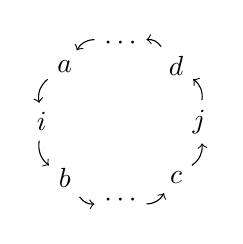
\begin{tikzpicture}
      \begin{scope}[shift={(0,0)}]
\node (0) at ({90 + (360/8 * 0)}:1) {\( \cdots \)};
\node (1) at ({90 + (360/8 * 1)}:1) {\( a \)};
\node (2) at ({90 + (360/8 * 2)}:1) {\( i \)};
\node (3) at ({90 + (360/8 * 3)}:1) {\( b \)};
\node (4) at ({90 + (360/8 * 4)}:1) {\( \cdots \)};
\node (5) at ({90 + (360/8 * 5)}:1) {\( c \)};
\node (6) at ({90 + (360/8 * 6)}:1) {\( j \)};
\node (7) at ({90 + (360/8 * 7)}:1) {\( d \)};
\draw[->,bend right] (0) to (1);
\draw[->,bend right] (1) to (2);
\draw[->,bend right] (2) to (3);
\draw[->,bend right] (3) to (4);
\draw[->,bend right] (4) to (5);
\draw[->,bend right] (5) to (6);
\draw[->,bend right] (6) to (7);
\draw[->,bend right] (7) to (0);
\end{scope}
    \end{tikzpicture} \qquad \qquad \qquad 
    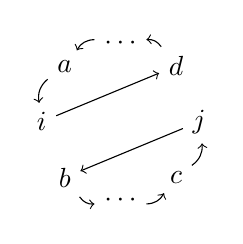
\begin{tikzpicture}
      \begin{scope}[shift={(0,0)}]
\node (0) at ({90 + (360/8 * 0)}:1) {\( \cdots \)};
\node (1) at ({90 + (360/8 * 1)}:1) {\( a \)};
\node (2) at ({90 + (360/8 * 2)}:1) {\( i \)};
\node (3) at ({90 + (360/8 * 3)}:1) {\( b \)};
\node (4) at ({90 + (360/8 * 4)}:1) {\( \cdots \)};
\node (5) at ({90 + (360/8 * 5)}:1) {\( c \)};
\node (6) at ({90 + (360/8 * 6)}:1) {\( j \)};
\node (7) at ({90 + (360/8 * 7)}:1) {\( d \)};
\draw[->,bend right] (0) to (1);
\draw[->,bend right] (1) to (2);
\draw[->] (2) to (7);
\draw[->,bend right] (3) to (4);
\draw[->,bend right] (4) to (5);
\draw[->,bend right] (5) to (6);
\draw[->] (6) to (3);
\draw[->,bend right] (7) to (0);
\end{scope}
    \end{tikzpicture}
    \caption{A cycle \( \rho \) with \( i \) and \( j \) on the left
      and the permutation \( \rho\tau \) on the right, where
      \( \tau=(i,j) \).}
    \label{fig:mult-tau}
  \end{figure}
\end{proof}


\begin{lem}\label{lem:inv+1}
  Let \( \pi\in \sym_n \) and let \( \tau=(i,i+1)\in\sym_n \). Then
  \[
    \sgn(\pi\tau) =  - \sgn(\pi).
  \]
\end{lem}

\begin{proof}
  Since
  \[
    \pi\tau =
    \begin{pmatrix}
      \cdots & i & i+1 & \cdots \\
      \cdots & \pi_{i+1} & \pi_i & \cdots 
    \end{pmatrix},
  \]
  we have \( \inv(\pi\tau) = \inv(\pi)\pm 1 \). This implies
  \( \sgn(\pi\tau) = - \sgn(\pi) \).
\end{proof}


\begin{lem}\label{lem:sgn=trans}
  If \( \pi\in \sym_n \) is a product of \( k \) simple transpositions, then
  \[
    \sgn(\pi) = (-1)^k.
  \]
\end{lem}
\begin{proof}
  Let \( \pi = t_1 \cdots t_k \), where \( t_i \)'s are simple
  transpositions. Then by \Cref{lem:sgn=trans},
  \[
    \sgn(\pi) = \sgn(\iota t_1 \cdots t_k) = (-1)^{k}\sgn(\iota) = (-1)^{k}.
  \]
\end{proof}

\begin{prop}
    For two permutations \( \pi,\sigma\in \sym_n \), we have
  \[
    \sgn(\pi\sigma) = \sgn(\pi) \sgn(\sigma).
  \]
\end{prop}
\begin{proof}
  Suppose \( \pi = t_1 \cdots t_k \) and
  \( \sigma = s_1 \cdots s_r \), where \( t_i \)'s and \( s_r \)'s are
  simple transpositions. Then since \( \sgn(\pi) = (-1)^{k} \)
  \( \sgn(\sigma) = (-1)^{r} \), we have
  \[
    \sgn(\pi\sigma) = \sgn(t_1 \cdots t_k s_1 \cdots s_r) = (-1)^{k+r}
    = \sgn(\pi) \sgn(\sigma). \qedhere
  \]
\end{proof}


\begin{prop}
  For \( \pi\in \sym_n \), we have
  \[
    \sgn(\pi) = (-1)^{\inv(\pi)} = (-1)^{n-\cycle(\pi)} =
    (-1)^{\evencycle(\pi)},
  \]
  where \( \evencycle(\pi) \) is the number of even cycles in
  \( \pi \). In particular, if \( \pi = t_1 \cdots t_k \), where
  \( t_i \)'s are transpositions, then \( \sgn(\pi) = (-1)^{t} \).
\end{prop}
\begin{proof}
  Let \( \pi = t_1 \cdots t_k \), where \( t_i \)'s are simple
  transpositions. By the definition of \( \sgn(\pi) \) and
  \Cref{lem:sgn=trans}, we have
  \( \sgn(\pi) = (-1)^{\inv(\pi)} = (-1)^{k} \). On the other hand,
  since \( \pi = t_1 \cdots t_k\iota \), by \Cref{lem:cycle+1},
  \( (-1)^{\cycle(\pi)} = (-1)^{\cycle(\iota)+k} = (-1)^{n+k} \).
  Thus \( \sgn(\pi) = (-1)^{k} = (-1)^{n-\cycle(\pi)} \).

  Now let \( c_i \) be the number of cycles of length \( i \) in
  \( \pi \). Then
  \[
    (-1)^{n-\cycle(\pi)} = (-1)^{(1\cdot c_1 + 2\cdot c_2 + \cdots + n
      \cdot c_n) - (c_1 + \cdots + c_n)} =(-1)^{0\cdot c_1 + 1\cdot
      c_2 + \cdots + (n-1) \cdot c_n} = (-1)^{n-\cycle(\pi)}.
  \]

  The last statement follows from
  \[
    \sgn(\pi) = \sgn(t_1 \cdots t_k) = \sgn(t_1) \cdots \sgn(t_k)
    = (-1)^{k},
  \]
  because the sign of a transposition \( \tau \) is
  \( \sgn(\tau) = (-1)^{\evencycle(\tau)} = (-1)^1 = -1 \).
\end{proof}

The \emph{signless Striling number of the first kind} \( c(n,k) \) is
defined to be the number of permutations on \( [n] \) with \( k \)
cycles. The \emph{Striling number of the first kind} \( s(n,k) \) is
defined to by \( s(n,k) = (-1)^{n-k} c(n,k) \). Note that
\( (-1)^{n-k} \) is the sign of a permutation on \( [n] \) with
\( k \) cycles.

\begin{prop}
  For integers \( n,k\ge1 \), we have
  \begin{equation}\label{eq:c(n,k)-rec}
    c(n,k) = c(n-1,k-1) + (n-1) c(n-1,k).
  \end{equation}
\end{prop}
\begin{proof}
  A permutation \( \pi \in \sym_n \) can be obtained from a
  permutation \( \pi'\in \sym_{n-1} \) by creating a new cycle
  \( (n) \) of length \( 1 \) or by inserting \( n \) after any
  integer in a cycle of \( \pi' \). For example, for
  \( \pi' = (1,9,3)(2,5)(4,8) (6) (7) \in \sym_9 \), if we insert
  \( 10 \) after \( 2 \), we get
  \( \pi = (1,9,3)(2,10,5)(4,8) (6) (7) \in \sym_{10} \), if we insert
  \( 10 \) after \( 6 \), we get
  \( \pi = (1,9,3)(2,5)(4,8) (6,10) (7) \in \sym_{10} \), and if we
  create a new cycle with \( 10 \), we get
  \( \pi = (1,9,3)(2,5)(4,8) (6) (7) (10) \in \sym_{10} \). This shows
  the recursion.
\end{proof}


\begin{prop}
  We have
  \begin{equation}\label{eq:s(n,k)}
    \sum_{k=0}^{n} s(n,k) x^k = (x)_n.
  \end{equation}
  Equivalently,
  \begin{equation}\label{eq:c(n,k)}
    \sum_{k=0}^{n} c(n,k) x^k = x(x+1) \cdots (x+n-1).
  \end{equation}
\end{prop}

\begin{proof}
  The equivalence of \eqref{eq:s(n,k)} and \eqref{eq:c(n,k)} is
  obtained by replacing \( x \) by \( -x \) and multiplying
  \( (-1)^{n} \) both sides.
  Thus it suffices to show \eqref{eq:c(n,k)}.
  This can be proved by induction using \eqref{eq:c(n,k)-rec}.
\end{proof}

Note that \eqref{eq:c(n,k)} can be rewritten as
\begin{equation}\label{eq:c(n,k)-gf}
   \sum_{\pi\in \sym_n}  x^{\cycle(\pi)} = x(x+1) \cdots (x+n-1).
\end{equation}
We can prove this bijectively.

\begin{proof}[A bijective proof of \eqref{eq:c(n,k)-gf}]
  We will construct an algorithm to construct a permutation
  \( \pi\in \sym_n \).
  For \( k=1,\dots,n \), we do the following.
  \begin{description}
  \item[Step 1] For \( k=1 \), create a new cycle consisting of \( 1 \).
  \item[Step 2] Let \( 2\le k\le n \) and suppose that the integers
    \( 1,\dots,k-1 \) form a permutation on \( [k-1] \) in cycle
    notation. Then we either create a new cycle consisting of \( k \)
    or insert \( k \) after one of the integers \( 1,\dots,k-1 \).
  \end{description}

  For each \( 1\le k\le n \), there are \( k \) choices: creating a
  new cycle (in one way) or inserting \( k \) into one of the existing
  cycles (in \( k-1 \) ways). The possible choices for \( k \) are
  exactly the same as the choices for the \( k \)th factor when we
  expand
  \begin{equation}\label{eq:19}
    x(x+1)(x+1+1)\cdots (x+\overbrace{1+1 + \cdots + 1}^{n-1}).
  \end{equation}
  Moreover, the first choice (creating a new cycle) corresponds to
  multipying \( x \). Thus, if \( \pi \) is a permutation obtained in
  this algoritm, then the same process in the exansion of
  \eqref{eq:19} gives \( x^{\cycle(\pi)} \). This means that the both
  sides of\eqref{eq:c(n,k)-gf} match term-by-term, completing the
  proof of this identity.
\end{proof}


Using \eqref{eq:S(n,k)(x)k=xn} and \eqref{eq:s(n,k)} we obtain the
following matrix identity, which is a duality between Stirling numbers
of the first and second kinds.


\begin{prop}
  We have
 \begin{equation}\label{eq:18}
   \Big(S(n,k)\Big)_{n,k\ge0} \Big(s(n,k)\Big)_{n,k\ge0} = I,
 \end{equation} 
 where \( I= (\delta_{n,k})_{n,k\ge0} \) is the infinite identity
 matrix.
 Equivalently, for integers \( n,m\ge0 \),
 \begin{align}
   \label{eq:S-s-dual}
   \sum_{k\ge0} S(n,k)s(k,m) & = \delta_{n,m},\\
   \label{eq:s-S-dual}
   \sum_{k\ge0} s(n,k)S(k,m) & = \delta_{n,m}.
 \end{align}
\end{prop}

\begin{proof}
  By \eqref{eq:S(n,k)(x)k=xn} and \eqref{eq:s(n,k)}, we have
  the change of basis identities between
  two bases \( \{x^n\}_{n\ge0} \) and \( \{(x)_n\}_{n\ge0} \)
  of the vector space of polynomials:
  \begin{align*}
   \Big(S(n,k)\Big)_{n,k\ge0} \Big((x)_n\Big)_{n\ge0} &=  \Big(x^n\Big)_{n\ge0},\\
   \Big(s(n,k)\Big)_{n,k\ge0} \Big(x^n\Big)_{n\ge0} &=  \Big((x)_n\Big)_{n\ge0}.
 \end{align*}
 Thus the two matrices \( (S(n,k))_{n,k\ge0} \) and
 \( (s(n,k))_{n,k\ge0} \) are inverse of each other, proving
 \eqref{eq:18}.
\end{proof}


\chapter{Combinatorial models for OPS}
\label{sec:comb-interpr-orth}

From now one we will focus on the combinatorial approaches to
orthogonal polynomials in Viennot's lecture notes \cite{ViennotLN}.
A part of this chapter has some overlaps with \Cref{sec:basics-orth-polyn}.

The main goal of this chapter to give combinatorial interpretations
for orthogonal polynomials and their moments. Using these
combinatorial interpretations, we will reprove the orthogonality of
orthogonal polynomials using combinatorics only.

\section{Orthogonal polynomials and 3-term recurrences}

In this section we recall basic definitions and properties of
orthogonal polynomials. We then state the 3-term recurrence of
orthogonal polynomials and Favard's theorem.

Let \( K \) be a field (we can also use a commutative ring for any
result without using divisions). We denote by \( K[x] \) the ring of
polynomials in \( x \) with coefficients in \( K \). A \emph{linear
  functional} is a linear transformation \( \LL:K[x]\to K \), i.e., a
function satisfying \( \LL(af(x)+bg(x)) = a \LL(f(x))+b \LL(g(x)) \)
for all \( f(x),g(x)\in K[x] \) and \( a,b\in K \). The \( n \)th
\emph{moment} of \( \LL \) is defined to be \( \mu_n = \LL(x^n) \).

\begin{defn}\label{def:formal-ops}
  Let \( \LL \) be a linear functional defined on the space of
  polynomials in \( x \). A sequence of polynomials
  \( \{P_n(x)\}_{n\ge0} \) is called an \emph{orthogonal polynomial
    sequence (OPS)} with respect to \( \LL \) if the following
  conditions hold:
  \begin{enumerate}
  \item \( \deg P_n(x) = n \), \( n\ge0 \),
  \item \( \LL(P_m(x)P_n(x))  = 0 \) for \( m\ne n \),
  \item \( \LL(P_m(x)^2) \ne 0 \) for \( m\ge0 \).
  \end{enumerate}
  We also say that \( \{ P_n(x) \}_{n\ge 0} \) is orthogonal
  for the moments \( \{\mu_n\}_{n\ge0} \).
\end{defn}

Orthogonal polynomials in the above definition are called ``formal''
or ``general'' orthogonal polynomials because the field \( K \) can be
anything. For instance, it may contain arbitrary formal variables such
as \( a,b,c,d \). Then the polynomials \( P_n(x) \) and the moments
\( \mu_n \) can be treated as polynomials (or more complicated objects
such as formal power series or rational functions) in these formal
variables.

\begin{prop}
  Suppose that \( \{ P_n(x) \}_{n\ge 0} \) is an OPS for \( \LL \).
\begin{enumerate}
\item \( \{ P_n(x) \}_{n\ge 0} \) is also orthogonal with respect to
  \( \LL' \) for any \( \LL' = a\LL \) for \( a\ne 0 \).
\item \( \LL \) is uniquely determined up to
  nonzero scalar multiplication. 
\item If we set \( \LL(1) = 1 \), then \( \LL \) is uniquely
  determined.
\item \( \{ a_nP_n(x) \}_{n\ge 0} \) is an OPS with respect to
  \( \LL \) for any sequence \( \{ a_n\}_{n\ge 0} \) with
  \( a_n\ne 0 \).
\end{enumerate}
\end{prop}

\begin{proof}
  All statements are easy to check. For example, (2) can be seen by
  noticing that once the \( 0 \)th moment \( \mu_0=\LL(1) \) is
  determined, then the \( n \)th moment \( \mu_n \), for \( n\ge1 \),
  is uniquely determined by the condition \( \LL(P_n(x)) = 0 \).
\end{proof}

By the above proposition we may assume that \( \LL(1) = 1 \).
\emph{From now on we will always assume that \( \deg P_n(x) = n \) and
  \( \LL(1) = 1 \) unless otherwise stated.}

Recall from \Cref{thm:3-RR} that every OPS satisfies a 3-term
recurrence.

\begin{thm}[3-term recurrence]
  Let \( \LL \) be a linear functional with monic OPS
  \( \{ P_n(x) \}_{n\ge 0} \). Then there are sequences
  \( \{ b_n\}_{n\ge 0} \) and \( \{ \lambda_n\}_{n\ge 1} \) such that
  \( \lambda_n\ne 0 \) and
  \[
    P_{n+1}(x) = (x-b_n) P_n(x) - \lambda_n P_{n-1}(x), \qquad n\ge0,
  \]
  where \( P_{-1}(x) = 0 \) and \( P_0(x) = 1 \).
\end{thm}

The inverse of the above theorem is also true, which is one of the
most important results in the theory of classical orthogonal
polynomials.

\begin{thm}[Favard's theorem]
  Let \( \{ P_n(x) \}_{n\ge 0} \) be a sequence of polynomials
  satisfying \( P_{-1}(x) = 0 \), \( P_0(x) = 1 \), and
  \begin{equation}\label{eq:3-RR}
    P_{n+1}(x) = (x-b_n) P_n(x) - \lambda_n P_{n-1}(x), \qquad n\ge0,
  \end{equation}
  for some sequences \( \{ b_n\}_{n\ge 0} \) and
  \( \{ \lambda_n\}_{n\ge 1} \) with \( \lambda_n\ne 0 \). 
 Then
  \( \{ P_n(x) \}_{n\ge 0} \) is an OPS for some linear functional
  \( \LL \).
\end{thm}

The main goal of this chapter is to give combinatorial interpretations
for the orthogonal polynomials \( P_n(x) \) and their moments
\( \mu_n \). Using these combinatorial interpretations we will prove
Favard's theorem bijectively.

\section{A model for orthogonal polynomials using Favard tilings}

In this section we give a combinatorial interpretation for
orthogonal polynomials using Favard tilings.


\begin{defn}
  A \emph{Favard tiling of size $n$} is a tiling of a $1\times n$
  square board with three types of tiles: red monominos, black
  monominos, and black dominos. The set of Favard tilings of size $n$
  is denoted by $\FT_n$.

  We label the squares in the $1\times n$ board by $0,1,\dots,n-1$
  from left to right. Define the weight \( \wt(T) \) of
  \( T\in \FT_n \) to be the product of the weights of the tiles in
  \( T \), where
  \begin{enumerate}
  \item the weight of each red monomino is \( x \),
  \item the weight of each black monomino containing a label
    \( i \) is \( -b_i \), and
  \item the weight of each domino containing labels \( i-1 \) and
    \( i \) is \( -\lambda_i \).
  \end{enumerate}




\end{defn}

For example, see \Cref{fig:tiling}. Note that the number \( u_n \) of
Favard tilings of size \( n \) satisfies \( u_{n+1} = 2u_n+u_{n-1} \)
with \( u_0=1 \) and \( u_1=2 \). These numbers are called the Pell
numbers.

\begin{figure}
  \centering
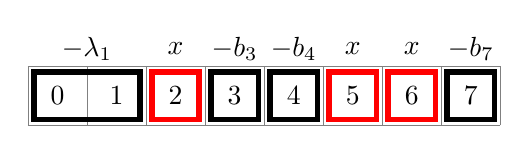
\begin{tikzpicture}[scale=0.75]
  \draw [help lines] (0,0) grid (8,1);
  \foreach \x in {0,...,7} \draw node at (\x+.5,.5) {\x};
  \LBD1 \LRM2 \LBM3 \LBM4 \LRM5 \LRM6 \LBM7
\end{tikzpicture}
\caption{A Favard tiling $T\in\FT_8$ with
  $\wt(T)=\lambda_1 b_3b_4b_7x^3$.}
  \label{fig:tiling}
\end{figure}

The following proposition gives a combinatorial interpretation for
orthogonal polynomials.

\begin{prop}\label{pro:Favard}
  Suppose that \( \{ P_n(x) \}_{n\ge 0} \) is a sequence of
  polynomials satisfying \eqref{eq:3-RR}. Then
  \[
    P_n(x) = \sum_{T\in \FT_n} \wt(T).
  \]
\end{prop}
\begin{proof}
  This is immediate from the recurrence \eqref{eq:3-RR}.
\end{proof}


\section{How to find a combinatorial model for moments}

Moments are important quantities of a linear functional \( \LL \)
because they have all the information of \( \LL \). In this section
we will find a combinatorial interpretation for the moments of
orthogonal polynomials. To do this we will first take a close look at
the moments.

Suppose that \( \LL \) is a linear functional with monic OPS
\( \{ P_n(x) \}_{n\ge 0} \), which satisfies the 3-term recurrence
\eqref{eq:3-RR}. Let's assume \( \LL(1)=1 \). Then, using the
orthogonality, we have
\begin{equation}\label{eq:13}
  \LL(P_n(x)) = \delta_{n,0}.
\end{equation}
This relation in fact completely determines the moments \( \mu_n \).
For example, since
\begin{align*}
  P_0(x) &= 1,\\
  P_1(x) &= (x-b_0)P_0(x) - \lambda_0P_{-1}(x) = x-b_0,\\
  P_2(x) &= (x-b_1)P_1(x) - \lambda_1P_0(x) =  x^2 - (b_1+b_0)x +b_0b_1 - \lambda_1,
\end{align*}
we have
\begin{align*}
 \mu_0 &= \LL(1) = 1, \\
 \mu_1 &= \LL(x) = \LL(P_1(x)+b_0) = b_0, \\
  \mu_2 &= \LL(x^2) = \LL(P_2(x)+(b_0+b_1)x-b_0b_1+\lambda_1)
          = (b_0+b_1)b_0 - b_0b_1 +\lambda_1 = b_0^2+\lambda_1.
\end{align*}
In this way, we can compute a few more moments:
\begin{align*}
  \mu_3 &= b_0^3 + 2b_0\lambda_1 + b_1\lambda_1,\\
  \mu_4 &= b_0^4 + 3b_0^2\lambda_1 + 2b_0b_1\lambda_1 + b_1^2\lambda_1 + \lambda_1^2 + \lambda_1\lambda_2,\\
  \mu_5 &= b_0^5 + 4b_0^3\lambda_1 + 3b_0^2b_1\lambda_1 + 2b_0b_1^2\lambda_1 + b_1^3\lambda_1 + 3b_0\lambda_1^2 + 2b_1\lambda_1^2 + 2b_0\lambda_1\lambda_2 + 2b_1\lambda_1\lambda_2 + b_2\lambda_1\lambda_2.
\end{align*}

The above experiments clearly suggest that \( \mu_n \) would be a
polynomial in \( b_i \)'s and \( \lambda_i \)'s with nonnegative
integer coefficients. How can we prove such a conjecture? A satisfying
answer to this question is to find combinatorial objects whose
generating function is \( \mu_n \). That is to find a set \( X \) of
combinatorial objects and a weight \( \wt(A) \) of each element
\( A\in X \) such that
\[
  \mu_n = \sum_{A \in X} \wt(A),
\]
and \( \wt(A) \) is a polynomial (preferably a monomial) in
\( b_i \)'s and \( \lambda_i \)'s with nonnegative integer
coefficients.

But how can we find such combinatorial objects? Suppose that such
combinatorial objects exist with monomial weight \( \wt(A) \) for each
\( A\in X \). Then if we set \( b_i=\lambda_i=1 \) for all \( i \)
then \( \mu_n \) would be the number of elements in \( X \). If we
compute \( \mu_n \) with this substitution for \( n=0,1,2,\ldots \),
then we obtain the following sequence:
\[
  1, 1, 2, 4, 9, 21, 51, 127, 323, 835, 2188, 5798, 15511, \ldots.
\]
There is a very useful webpage \url{https://oeis.org/} where you can
search integer sequences. If you search the above sequence, the
webpage will tell you that this is the sequence of the number of
Motzkin paths. So we can guess that there must be a close connection
with the moments of orthogonal polynomials and Motzkin paths.

After spending enough time of trials and errors, we can come up with
the following combinatorial model for the moments of orthogonal
polynomials.

Recall that \( \Motz(u\to v) \) is the set of Motzkin paths from
\( u \) to \( v \). We define the weight \( \wt(\pi) \) of a Motzkin
path \( \pi \) to be the product of the weights of the steps in
\( \pi \), where
\begin{enumerate}
\item the weight of an up step is \( 1 \),
\item the weight of a horizontal step starting at height \( i \) is \( b_i \), and
\item the weight of a down step starting at height \( i \) is
  \( \lambda_i \).
\end{enumerate}
See \Cref{fig:Motzkin-wt}.

\begin{figure}
  \centering
  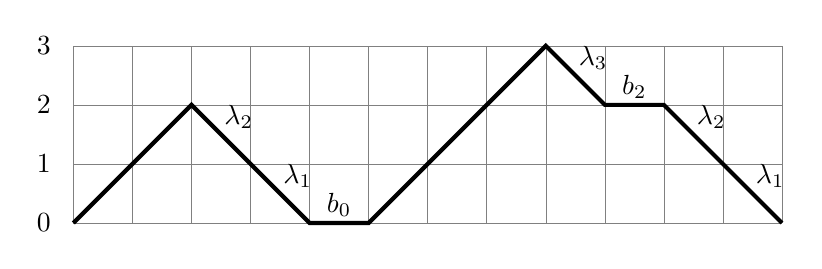
\begin{tikzpicture}[scale=0.75]
    \draw[help lines] (0,0) grid (12,3);
    \foreach \y in {0,...,3} \draw node at (-.5,\y) {$\y$};
\draw[line width = 1.5pt] (0,0) -- ++(1,1) -- ++(1,1) -- ++(1,-1) -- ++(1,-1) -- ++(1,0) -- ++(1,1) -- ++(1,1) -- ++(1,1) -- ++(1,-1) -- ++(1,0) -- ++(1,-1) -- ++(1,-1);
    \node at (2.8,1.8) {$\lambda_{2}$};
    \node at (3.8,0.8) {$\lambda_{1}$};
    \node at (4.5,0.3) {$b_{0}$};
    \node at (8.8,2.8) {$\lambda_{3}$};
    \node at (9.5,2.3) {$b_{2}$};
    \node at (10.8,1.8) {$\lambda_{2}$};
    \node at (11.8,0.8) {$\lambda_{1}$};
\end{tikzpicture}
\caption{A Motzkin path $\pi$ from $(0,0)$ to $(12,0)$ with
  $\wt(\pi)=b_0b_2\lambda_1^2\lambda_2^2\lambda_3$.}
  \label{fig:Motzkin-wt}
\end{figure}

We are now ready state Viennot's combinatorial interpretation for
moments of orthogonal polynomials.

\begin{thm}\label{thm:mu=Mot}
  Suppose that \( \{ P_n(x) \}_{n\ge 0} \) is a monic OPS for a
  linear functional \( \LL \) with \( \LL(1)=1 \). Suppose that
  \( \{ P_n(x) \}_{n\ge 0} \) satisfy the 3-term recurrence
  \[
      P_{n+1}(x) = (x-b_n) P_n(x) - \lambda_n P_{n-1}(x), \qquad n\ge0.
  \]
  Then the moments \( \mu_n=\LL(x^n) \) are given by
\[
  \mu_n = \sum_{\pi\in \Motz_n} \wt(\pi).
\]
\end{thm}

More generally, we will prove
a combinatorial interpretation for mixed moments.

\begin{defn}
  Let \( \{ P_n(x) \}_{n\ge 0} \) be a monic OPS for a linear
  functional \( \LL \). For integers \( n,r,s\ge0 \), the \emph{mixed
    moments} \( \mu_{n,r,s} \) and \( \mu_{n,k} \) of this OPS are
  defined by
  \begin{align*}
    \mu_{n,r,s} &= \frac{\LL(x^n P_r(x)P_s(x))}{\LL(P_s(x)^2)},\\
    \mu_{n,k} &= \mu_{n,0,k} = \frac{\LL(x^n P_k(x))}{\LL(P_k(x)^2)}.
  \end{align*}
\end{defn}

Note that \( \mu_n = \mu_{n,0,0} \).

Let \( \Motz_{n,r,s} \) denote the set of Motzkin paths from
\( (0,r) \) to \( (n,s) \). 

\begin{thm}\label{thm:mu=Mot_nrs}
  Following the notation in \Cref{thm:mu=Mot}, we have
\[
  \mu_{n,r,s} = \sum_{\pi\in \Motz_{n,r,s}} \wt(\pi).
\]
\end{thm}

\begin{proof}
  We proceed by induction on \( n \).
  Suppose \( n=0 \). By the orthogonality of \( \{ P_n(x) \}_{n\ge 0} \),
  we have
  \[
    \mu_{0,r,s} = \frac{\LL(P_r(x)P_s(x))}{\LL(P_s(x)^2)} = \delta_{r,s}.
  \]
  Since \( \Motz_{0,r,s} = \emptyset \) if \( r=s \) and
  \( \Motz_{0,r,s} \) has only one (empty) Motzkin path if \( r=s \),
  we also have
  \( \sum_{\pi\in \Motz_{n,r,s}} \wt(\pi) = \delta_{r,s} \).

  Let \( n\ge1 \) and suppose that the theorem holds for \( n-1 \).
  Then by the 3-term recurrence,
  \[
    xP_r(x) = P_{r+1}(x) + b_rP_r(x) + \lambda_rP_{r-1}(x).
  \]
  Thus
  \begin{align*}
    \mu_{n,r,s}
    &= \frac{\LL(x^n P_r(x) P_s(x))}{\LL(P_s(x)^2)}
      = \frac{\LL(x^{n-1} (xP_r(x)) P_s(x))}{\LL(P_s(x)^2)}\\
    &=\frac{\LL(x^{n-1} (P_{r+1}(x) + b_rP_r(x) + \lambda_rP_{r-1}(x)) P_s(x))}{\LL(P_s(x)^2)} \\
    &= \frac{\LL(x^{n-1} P_{r+1}(x)P_s(x))}{\LL(P_s(x)^2)}
      + b_r\frac{\LL(x^{n-1} P_r(x)P_s(x))}{\LL(P_s(x)^2)}
      + \lambda_r \frac{\LL(x^{n-1} P_{r-1}(x)P_s(x))}{\LL(P_s(x)^2)}\\
    &= \mu_{n-1,r+1,s} + b_r\mu_{n-1,r,s} + \lambda_r \mu_{n-1,r-1,s}\\
    &= \sum_{\pi\in \Motz_{n-1,r+1,s}} \wt(\pi)
    + b_r \sum_{\pi\in \Motz_{n-1,r,s}} \wt(\pi)
    + \lambda_r \sum_{\pi\in \Motz_{n-1,r-1,s}} \wt(\pi)\\
      &=      \sum_{\pi\in \Motz_{n,r,s}} \wt(\pi),
  \end{align*}
  where the second to last equation follows from the induction
  hypothesis and the last equation follows from considering the first
  step of each \( \pi\in \Motz_{n,r,s} \). Hence the theorem holds for
  \( n \) and we are done by induction.
\end{proof}

\begin{cor}
  Following the notation in \Cref{thm:mu=Mot}, we have
  \[
    \LL(P_n(x)^2) = \lambda_1 \cdots \lambda_n.
  \]
\end{cor}

\begin{proof}
  Since \( P_n(x) \) is monic, we can write \( P_n(x) = x^n + Q(x) \)
  for some polynomial \( Q(x) \) of degree less than \( n \). Thus
  by \Cref{thm:mu=Mot_nrs},
  \[
    \LL(P_n(x)^2) = \LL((x^n + Q(x))P_n(x)) = \LL(x^n P_n(x))
    = \sum_{\pi\in \Motz_{n,n,0}} \wt(\pi) = \lambda_1 \cdots \lambda_n,
  \]
  as desired. Here, the last equality follows from the fact that there
  is only one Motzkin path in \( \Motz_{n,n,0} \), namely, the path
  from \( (0,n) \) to \( (n,0) \) consisting of \( n \) down steps.
\end{proof}

\section{A bijective proof of Favard's theorem}

We have a combinatorial interpretation for both orthogonal polynomials
and their moments. In this section we will prove Favard's theorem
bijectively using these combinatorial models.


Suppose that \( \{ P_n(x) \}_{n\ge 0} \) is a sequence of polynomials
satisfying the 3-term recurrence
\[
  P_{n+1}(x) = (x-b_n) P_n(x) - \lambda_n P_{n-1}(x).
\]
To prove Favard's theorem, we need to find a linear functional
\( \LL \) for which \( \{ P_n(x) \}_{n\ge 0} \) are orthogonal.
We simply define \( \LL \) so that the moments are given by
\begin{equation}\label{eq:8}
  \LL(x^n) = \sum_{\pi\in \Motz_{n}} \wt(\pi).
\end{equation}
It is enough to show that
\[
  \LL(P_r(x)P_s(x)) = \lambda_1 \cdots \lambda_s \delta_{r,s}.
\]
More generally, we will prove
\begin{equation}\label{eq:LL(xPP)}
  \LL(x^n P_r(x)P_s(x)) = \lambda_1 \cdots \lambda_s \sum_{\pi\in
    \Motz_{n,r,s}} \wt(\pi).
\end{equation}

We first need to give a combinatorial meaning to the the left-hand
side of \eqref{eq:LL(xPP)}. For a Favard tiling \( T \) with \( k \)
red monominos, let \( \wt'(T) = \wt(T)/x^k \). In other words,
\( \wt'(T) \) is the same as \( \wt(T) \) except we only consider the
weights of black monominos and black dominos.
Then \Cref{pro:Favard} can be restated as
\[
  P_n(x) = \sum_{T\in \FT_n} \wt'(T) \cdot x^{(\text{number of red monominos in \( T \)})}.
\]
Thus, by the definition of \( \LL(x^n) \) in \eqref{eq:8}, we have
\[
    \LL(x^n P_r(x)P_s(x)) = 
    \sum_{(T_1,T_2,\pi)\in X} \wt'(T_1) \wt'(T_2) \wt(\pi),
\]
where \( X \) is the set of triples \( (T_1,T_2,\pi) \)
such that for some \( 0\le i\le r \) and \( 0\le j\le s \),
\begin{enumerate}
\item \( T_1\in \FT_r \) has \( i \) red monominos,
\item \( T_2\in \FT_s \) has \( j \) red monominos, and
\item \( \pi\in \Motz_{n+i+j} \).
\end{enumerate}

Let \( Y \) be the set of \( \pi\in \Motz_{n+r+s} \) such that the
first \( r \) steps are up steps and the last \( s \) step s are down
steps. Then the right-hand side of \eqref{eq:LL(xPP)} is equal to
\( \sum_{\pi\in Y} \wt(\pi) \). Therefore \eqref{eq:LL(xPP)} is
equivalent to the following theorem.

\begin{thm}
  For the sets \( X \) and \( Y \) defined above, we have
\begin{equation}\label{eq:LL(xPP)2}
  \sum_{(T_1,T_2,\pi)\in X} \wt'(T_1) \wt'(T_2) \wt(\pi)
  =  \sum_{\pi\in Y} \wt(\pi).
\end{equation}
\end{thm}

\begin{proof}
  We will find a sign-reversing weight-preserving involution on
  \( X \) with fixed point set
  \( \{ (\emptyset,\emptyset,\pi):\pi\in Y\} \). Consider
  \( (T_1,T_2,\pi)\in X \). We write \( \pi=S_1S_2 \cdots S_{m} \) as
  a sequence of steps. Let \( a,b,u,v \) be the integers defined as follows:
 \begin{itemize}
 \item \( a \) is the largest integer such that \( T_1 \)
   starts with \( a \) red monominos,
 \item \( b \) is the largest integer such that \( T_2 \)
   starts with \( b \) red monominos,
 \item \( u \) is the largest integer such that \( \pi \) starts with
   \( u \) up steps,
 \item \( v \) is the largest integer such that \( \pi \) ends with
   \( v \) down steps.
 \end{itemize}

 We now define \( \phi(T_1,T_2,\pi)= (T'_1,T'_2,\pi') \) in the following
 way. Here, \( a',b',u',v' \) are the integers defined similarly as
 above using \( T'_1 \), \( T'_2 \), and \( \pi' \).
\begin{description}
\item[Case 1] \( u<a \). In this case we set \( T'_2 = T_2 \). There are two
  subcases.
\begin{description}
\item[Case 1-1] \( S_{u+1} \) is a horizontal step. Let
    \[
      \pi' = S_1\cdots \widehat{S_{u+1}} \cdots S_{m},
\]
and define $T_1'$ to be the Favard tiling obtained from $T_1$ by
replacing the \( (u+1) \)st red monomino (at position \( u \)) by a
black monomino. Here the notation $\widehat{S_{u+1}}$ means that
$S_{u+1}$ is removed from the sequence. See Figure~\ref{fig:case-1}.
Observe that since \( \wt'(T'_1) = -b_u \wt'(T_1) \) and
\( \wt'(\pi') = \wt'(\pi)/ b_u \), we have
\[ \wt'(T'_1)\wt'(T'_2)\wt(\pi') = - \wt'(T_1)\wt'(T_2)\wt(\pi). \]
Moreover, we always have \( u'\ge u \) and \( a'=u<a\le r \), hence
\( u'\ge a'\ne r \).
\item[Case 1-2] $S_{u+1}$ is a down step. Let
    \[
      \pi' = S_1\cdots \widehat{S_{u}}\widehat{S_{u+1}} \cdots S_m,
\]
and define $T_1'$ to be the Favard tiling obtained from $T_1$ by
replacing the \( u \)th and \( (u+1) \)st red monominos (at positions
$u-1$ and $u$) by a domino. See Figure~\ref{fig:case-2}. 
Observe that since \( \wt'(T'_1) = -\lambda_u \wt'(T_1) \) and
\( \wt'(\pi') = \wt'(\pi)/ \lambda_u \), we have
\[ \wt'(T'_1)\wt'(T'_2)\wt(\pi') = - \wt'(T_1)\wt'(T_2)\wt(\pi). \]
Moreover, we always have \( u'\ge u-1 \) and \( a'=u-1<a\le r \),
hence \( u'\ge a'\ne r \).
\end{description}

\item[Case 2] \( u\ge a\ne r \). In this case we set \( T'_2=T_2 \). Let
  \( A \) be the \( (a+1) \)st tile in \( T_1 \) (\( A \) starts at position
  \( a \)). There are two subcases.
  \begin{description}
  \item[Case 2-1] $A$ is a black monomino. In this case let
    \[
      \pi' = S_1\cdots S_u H S_{u+1} \cdots S_m,
\]
and define $T_1'$ to be the Favard tiling obtained from $T_1$ by
replacing $A$ by a red monomino. See Figure~\ref{fig:case-1} (with the
roles of \( (T_1,T_2,\pi) \) and \( (T'_1,T'_2,\pi') \) interchanged).
\item[Case 2-2] $A$ is a domino. In this case let
    \[
      \pi' = S_1\dots S_u UD S_{u+1} \dots S_m,
\]
and define $T_1'$ to be the Favard tiling obtained from $T_1$ by
replacing $A$ by two red monominos. See Figure~\ref{fig:case-2} (with
the roles of \( (T_1,T_2,\pi) \) and \( (T'_1,T'_2,\pi') \)
interchanged).
\end{description}
\item[Case 3] \( u\ge a = r \) and \( v<b \). This can be done
  similarly as Case 1. The only difference is that we set
  \( T_1' = T_1 \) and consider the steps of \( \pi \) from the right.
  
\item[Case 4] \( u\ge a = r \) and \( v\ge b \ne s \).
  This can be done similarly as Case 2.

\item[Case 5] \( u\ge a = r \) and \( v\ge b=s \). In this case we set
  \( (T'_1,T'_2,\pi') = (T_1,T_2,\pi) \). See \Cref{fig:case5}.
\end{description}

\begin{figure}
  \centering
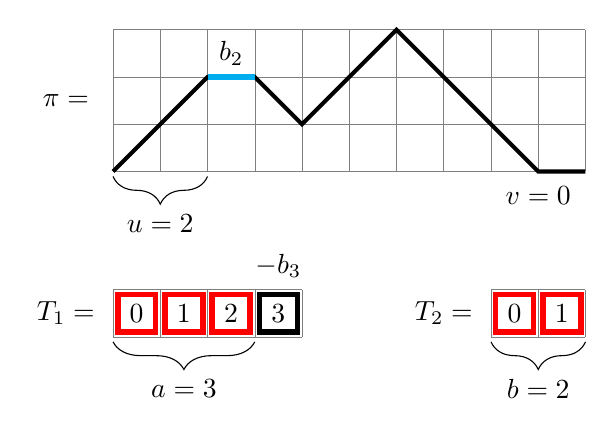
\begin{tikzpicture}[scale=0.6]
  \draw[help lines] (0,0) grid (10,3);
\draw[line width = 1.5pt] (0,0) -- ++(1,1) -- ++(1,1) -- ++(1,0) -- ++(1,-1) -- ++(1,1) -- ++(1,1) -- ++(1,-1) -- ++(1,-1) -- ++(1,-1) -- ++(1,0);
  \draw [decorate,decoration={brace,amplitude=10pt},xshift=-0pt,yshift=-3pt]
(2,0) -- (0,0) node [black,midway,yshift=-0.6cm] {\( u=2 \)};
\node at (-1,1.5) {\( \pi= \)};
\node at (9,-.5) {\( v=0 \)};
\node at (2.5,2.5) {\( b_2 \)};
\draw[line width = 2pt, cyan] (2,2)--++(1,0);
\begin{scope}[shift={(0,-3.5)}]
  \draw [help lines] (0,0) grid (4,1);
  \foreach \x in {0,...,3} \draw node at (\x+0.5,0.5) {\x};
  \RM0 \RM1 \RM2 \BM3
  \node at (3.5,1.5) {\( -b_3 \)};
  \draw [decorate,decoration={brace,amplitude=10pt},xshift=-0pt,yshift=-3pt]
(3,0) -- (0,0) node [black,midway,yshift=-0.6cm] {\( a=3 \)};
\node at (-1,.5) {\( T_1= \)};
\end{scope}
\begin{scope}[shift={(8,-3.5)}]
  \draw [help lines] (0,0) grid (2,1);
  \foreach \x in {0,...,1} \draw node at (\x+0.5,0.5) {\x};
  \RM0 \RM1
  \draw [decorate,decoration={brace,amplitude=10pt},xshift=-0pt,yshift=-3pt]
(2,0) -- (0,0) node [black,midway,yshift=-0.6cm] {\( b=2 \)};
\node at (-1,.5) {\( T_2= \)};
\end{scope}
\end{tikzpicture} \quad
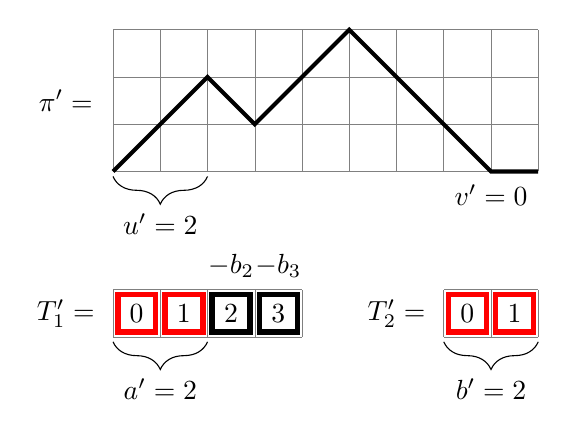
\begin{tikzpicture}[scale=0.6]
  \draw[help lines] (0,0) grid (9,3);
\draw[line width = 1.5pt] (0,0) -- ++(1,1) -- ++(1,1) -- ++(1,-1) -- ++(1,1) -- ++(1,1) -- ++(1,-1) -- ++(1,-1) -- ++(1,-1) -- ++(1,0);
  \draw [decorate,decoration={brace,amplitude=10pt},xshift=-0pt,yshift=-3pt]
(2,0) -- (0,0) node [black,midway,yshift=-0.6cm] {\( u'=2 \)};
\node at (-1,1.5) {\( \pi'= \)};
\remove(2,2)
\node at (8,-.5) {\( v'=0 \)};
\begin{scope}[shift={(0,-3.5)}]
  \draw [help lines] (0,0) grid (4,1);
  \foreach \x in {0,...,3} \draw node at (\x+0.5,0.5) {\x};
  \RM0 \RM1 \BM2 \BM3
  \draw [decorate,decoration={brace,amplitude=10pt},xshift=-0pt,yshift=-3pt]
(2,0) -- (0,0) node [black,midway,yshift=-0.6cm] {\( a'=2 \)};
\node at (-1,.5) {\( T'_1= \)};
  \node at (2.5,1.5) {\( -b_2 \)};
  \node at (3.5,1.5) {\( -b_3 \)};
\end{scope}
\begin{scope}[shift={(7,-3.5)}]
  \draw [help lines] (0,0) grid (2,1);
  \foreach \x in {0,...,1} \draw node at (\x+0.5,0.5) {\x};
  \RM0 \RM1
  \draw [decorate,decoration={brace,amplitude=10pt},xshift=-0pt,yshift=-3pt]
(2,0) -- (0,0) node [black,midway,yshift=-0.6cm] {\( b'=2 \)};
\node at (-1,.5) {\( T'_2= \)};
\end{scope}
\end{tikzpicture}  
\caption{A triple \( (\pi,T_1,T_2)\in X \) in Case 1-1 on the left and
  the corresponding triple \( (\pi',T'_1,T'_2)\in X \) in Case 2-1 on
  the right, where \( r=4 \), \( s=2 \), and \( n=5 \). The horizontal
  step \( (2,2)\to(3,3) \) in \( \pi \) is collapsed to a point.}
  \label{fig:case-1}
\end{figure}

\begin{figure}
  \centering
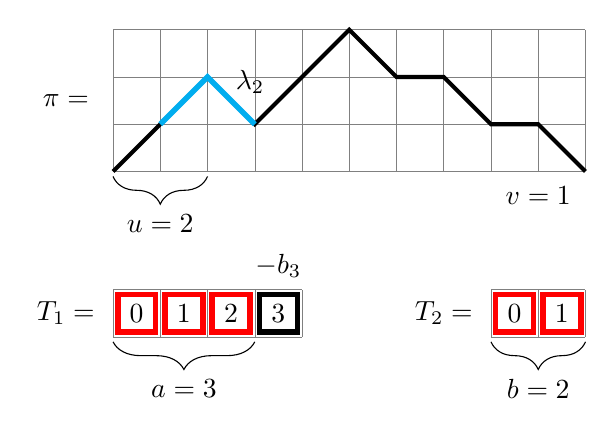
\begin{tikzpicture}[scale=0.6]
  \draw[help lines] (0,0) grid (10,3);
\draw[line width = 1.5pt] (0,0) -- ++(1,1) -- ++(1,1) -- ++(1,-1) -- ++(1,1) -- ++(1,1) -- ++(1,-1) -- ++(1,0) -- ++(1,-1) -- ++(1,0) -- ++(1,-1);
  \draw [decorate,decoration={brace,amplitude=10pt},xshift=-0pt,yshift=-3pt]
(2,0) -- (0,0) node [black,midway,yshift=-0.6cm] {\( u=2 \)};
\node at (-1,1.5) {\( \pi= \)};
\node at (9,-.5) {\( v=1 \)};
\node at (2.9,1.9) {\( \lambda_2 \)};
\draw[line width = 2pt, cyan] (1,1) -- (2,2)--++(1,-1);
\begin{scope}[shift={(0,-3.5)}]
  \draw [help lines] (0,0) grid (4,1);
  \foreach \x in {0,...,3} \draw node at (\x+0.5,0.5) {\x};
  \RM0 \RM1 \RM2 \BM3
  \draw [decorate,decoration={brace,amplitude=10pt},xshift=-0pt,yshift=-3pt]
(3,0) -- (0,0) node [black,midway,yshift=-0.6cm] {\( a=3 \)};
\node at (-1,.5) {\( T_1= \)};
\node at (3.5,1.5) {\( -b_3 \)};
\end{scope}
\begin{scope}[shift={(8,-3.5)}]
  \draw [help lines] (0,0) grid (2,1);
  \foreach \x in {0,...,1} \draw node at (\x+0.5,0.5) {\x};
  \RM0 \RM1
  \draw [decorate,decoration={brace,amplitude=10pt},xshift=-0pt,yshift=-3pt]
(2,0) -- (0,0) node [black,midway,yshift=-0.6cm] {\( b=2 \)};
\node at (-1,.5) {\( T_2= \)};
\end{scope}
\end{tikzpicture} \quad
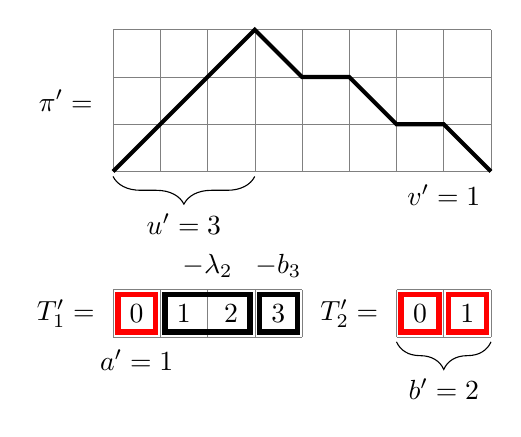
\begin{tikzpicture}[scale=0.6]
  \draw[help lines] (0,0) grid (8,3);
\draw[line width = 1.5pt] (0,0) -- ++(1,1) -- ++(1,1) -- ++(1,1) -- ++(1,-1) -- ++(1,0) -- ++(1,-1) -- ++(1,0) -- ++(1,-1);
  \draw [decorate,decoration={brace,amplitude=10pt},xshift=-0pt,yshift=-3pt]
(3,0) -- (0,0) node [black,midway,yshift=-0.6cm] {\( u'=3 \)};
\node at (-1,1.5) {\( \pi'= \)};
\remove(1,1)
\node at (7,-.5) {\( v'=1 \)};
\begin{scope}[shift={(0,-3.5)}]
  \draw [help lines] (0,0) grid (4,1);
  \foreach \x in {0,...,3} \draw node at (\x+0.5,0.5) {\x};
  \RM0 \BD2 \BM3
\node at (-1,.5) {\( T'_1= \)};
\node at (.5,-.5) {\( a'=1 \)};
\node at (3.5,1.5) {\( -b_3 \)};
\node at (2,1.5) {\( -\lambda_2 \)};
\end{scope}
\begin{scope}[shift={(6,-3.5)}]
  \draw [help lines] (0,0) grid (2,1);
  \foreach \x in {0,...,1} \draw node at (\x+0.5,0.5) {\x};
  \RM0 \RM1
  \draw [decorate,decoration={brace,amplitude=10pt},xshift=-0pt,yshift=-3pt]
(2,0) -- (0,0) node [black,midway,yshift=-0.6cm] {\( b'=2 \)};
\node at (-1,.5) {\( T'_2= \)};
\end{scope}
\end{tikzpicture}  
\caption{A triple \( (\pi,T_1,T_2)\in X \) in Case 1-2 on the left and
  the corresponding triple \( (\pi',T'_1,T'_2)\in X \) in Case 2-2 on
  the right, where \( r=4 \), \( s=2 \), and \( n=5 \). The peak (an
  upstep followed by a down step) \( (1,1)\to (2,2)\to(3,1) \) in
  \( \pi \) is collapsed to a point.}
  \label{fig:case-2}
\end{figure}

\begin{figure}
  \centering
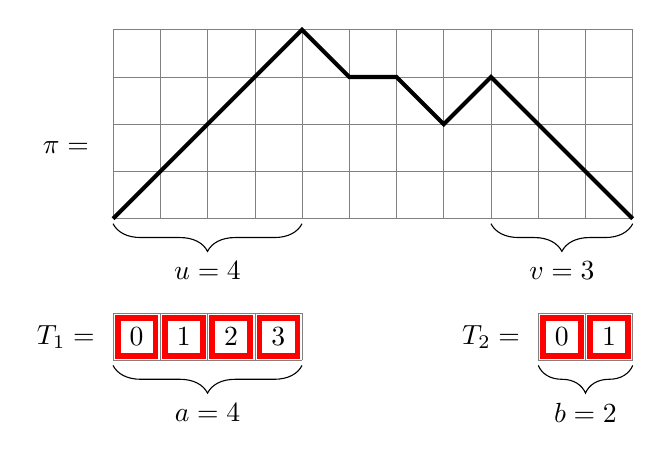
\begin{tikzpicture}[scale=0.6]
  \draw[help lines] (0,0) grid (11,4);
\draw[line width = 1.5pt] (0,0) -- ++(1,1) -- ++(1,1) -- ++(1,1) -- ++(1,1) -- ++(1,-1) -- ++(1,0) -- ++(1,-1) -- ++(1,1) -- ++(1,-1) -- ++(1,-1) -- ++(1,-1);
  \draw [decorate,decoration={brace,amplitude=10pt},xshift=-0pt,yshift=-3pt]
(4,0) -- (0,0) node [black,midway,yshift=-0.6cm] {\( u=4 \)};
\node at (-1,1.5) {\( \pi= \)};
  \draw [decorate,decoration={brace,amplitude=10pt},xshift=-0pt,yshift=-3pt]
(11,0) -- (8,0) node [black,midway,yshift=-0.6cm] {\( v=3 \)};
\begin{scope}[shift={(0,-3)}]
  \draw [help lines] (0,0) grid (4,1);
  \foreach \x in {0,...,3} \draw node at (\x+0.5,0.5) {\x};
  \RM0 \RM1 \RM2 \RM3
  \draw [decorate,decoration={brace,amplitude=10pt},xshift=-0pt,yshift=-3pt]
(4,0) -- (0,0) node [black,midway,yshift=-0.6cm] {\( a=4 \)};
\node at (-1,.5) {\( T_1= \)};
\end{scope}
\begin{scope}[shift={(9,-3)}]
  \draw [help lines] (0,0) grid (2,1);
  \foreach \x in {0,...,1} \draw node at (\x+0.5,0.5) {\x};
  \RM0 \RM1
  \draw [decorate,decoration={brace,amplitude=10pt},xshift=-0pt,yshift=-3pt]
(2,0) -- (0,0) node [black,midway,yshift=-0.6cm] {\( b=2 \)};
\node at (-1,.5) {\( T_2= \)};
\end{scope}
\end{tikzpicture}
\caption{A triple \( (\pi,T_1,T_2)\in X \) in Case 5, where \( r=4 \),
  \( s=2 \), and \( n=5 \).}
  \label{fig:case5}
\end{figure}

By the construction, Case 1 corresponds to Case 2 and Case 3
corresponds to Case 4. Thus the map
\( \phi(T_1,T_2,\pi)= (T'_1,T'_2,\pi') \) is a sign-reversing
weight-preserving involution on \( X \) with fixed points
\( (\emptyset,\emptyset,\pi) \) where \( \pi\in Y \). This completes
the proof.
\end{proof}

\chapter{Moments of classical orthogonal polynomials}

In this chapter we apply the combinatorial interpretation of moments
for Tchebyshev polynomials of the 1st and 2nd kinds, Hermite
polynomials, Charlier polynomials, and Laguerre polynomials.

Note that a monic OPS \( \{ P_n(x) \}_{n\ge 0} \) can be defined in
many ways, namely, one of the following determines the orthogonal
polynomials:
\begin{enumerate}
\item the coefficients \( \{a_{n,k}\}_{n,k\ge0} \) of \( P_n(x)= \sum_{k=0}^{n} a_{n,k} x^k   \),
\item the generating function \( \sum_{n\ge0}P_n(x)t^n \)
  or \( \sum_{n\ge0}P_n(x)t^n/n! \),
\item the moments \( \{ \mu_n\}_{n\ge 0} \),
\item the 3-term recurrence coefficients \( \{ b_n\}_{n\ge 0} \) and
  \( \{ \lambda_n\}_{n\ge 1} \).
\end{enumerate}

\section{Tchebyshev polynomials}

In this section we will compute the moments of Tchebyshev polynomials
using \Cref{thm:mu=Mot}. We will first consider Tchebyshev polynomials
of the second kind since they are simpler than the first kind in our
approach.



The \emph{Tchebyshev polynomials of the second kind}
\( U_n(x) \) are defined by
\[
  U_n(x) = \frac{\sin(n+1)\theta}{\sin\theta}, \qquad x=\cos\theta,
  \qquad n\ge0.
\]
They satisfy
  \[
    U_{n+1}(x) = 2x U_n(x) - U_{n-1}(x), \qquad n\ge0,
  \]
  where \( U_{-1}(x) = 0 \) and \( U_0(x) = 1 \).
  Using calculus we can prove that
  \[
    \int_{-1}^1 U_m(x)U_n(x) (1-x^2)^{1/2} dx = \frac{\pi}{2}\delta_{m,n}.
  \]
  Let \( \LL \) be the linear functional defined by
  \[
    \LL(f(x)) = \frac{2}{\pi} \int_{-1}^1 f(x) (1-x^2)^{1/2} dx.
  \]
  Then \( \{U_n(x)\}_{n\ge0} \) is an OPS for \( \LL \) and
  \( \LL(1) = 1 \).

  Since \( U_n(x) \) has leading coefficient \( 2^n \), the monic
  Tchebyshev polynomials \( \hat{U}_n(x) \) are given by
  \( \hat{U}_n(x) = 2^{-n}U_n(x) \) and
  \[
    \hat{U}_{n+1}(x) = (x-b_n) \hat{U}_n(x) - \lambda_n \hat{U}_{n-1}(x), \qquad n\ge0,
  \] 
  where \( b_n = 0 \) and \( \lambda_n = 1/4 \).

  Note that \( \{\hat{U}_n(x)\}_{n\ge0} \) is also an OPS for
  \( \LL \). Using calculus we can prove that
  the moments
  \[
    \mu_n= \LL(x^n) = \frac{2}{\pi} \int_{-1}^1 x^n (1-x^2)^{1/2} dx
  \]
  are given by
  \begin{equation}\label{eq:20}
    \mu_{2n} = \frac{1}{4^n} C_n, \qquad \mu_{2n+1} = 0.
  \end{equation}
  We will prove this combinatorially using the combinatorial
  interpretation for \( \mu_n \).

  By \Cref{thm:mu=Mot},
  \[
    \mu_n = \sum_{\pi\in \Motz_n} \wt(\pi)
    = \sum_{\pi\in \Dyck_n} \left( \frac{1}{4} \right)^{n/2}.
  \]
  Thus
  \[
    \mu_{2n} = \frac{1}{4^n} |\Dyck_{2n}|, \qquad \mu_{2n+1} = 0.
  \]
  This is the same as \eqref{eq:20}.

  \medskip

  Now we consider the Tchebyshev polynomials of the first kind,
  \( T_n(x) = \cos n\theta \), \( x=\cos \theta \). Recall that
\[
  \int_{-1}^1 T_m(x)T_n(x) (1-x^2)^{-1/2} dx = 0, \qquad m\ne n.
\]
  Let \( \LL \) be the linear functional defined by
  \[
    \LL(f(x)) = \frac{1}{\pi} \int_{-1}^1 f(x) (1-x^2)^{-1/2} dx.
  \]
  Then \( \{T_n(x)\}_{n\ge0} \) is an OPS for \( \LL \) and
  \( \LL(1) = 1 \). The moments
  \[
    \mu_n= \LL(x^n) = \frac{1}{\pi} \int_{-1}^1 x^n (1-x^2)^{-1/2} dx
  \]
  are given by
  \begin{equation}\label{eq:21}
    \mu_{2n} = \frac{1}{2^{2n}} \binom{2n}{n}, \qquad
    \mu_{2n+1} = 0.
  \end{equation}
  We will prove this combinatorially.

  The monic Tchebyshev polynomials of the first kind are given by
  \( \hat{T}_0(x) = 1 \) and \( \hat{T}_n(x) = 2^{1-n}T_n(x) \) for
  \( n\ge1 \). We have
  \[
      \hat{T}_{n+1}(x) = (x-b_n) \hat{T}_n(x) - \lambda_n\hat{T}_{n-1}(x),
      \qquad n\ge0,
  \]
  where \( b_n=0 \) for \( n\ge0 \), \( \lambda_1 = 1/2 \), and
  \( \lambda_n = 1/4 \) for \( n\ge2 \).


  By \Cref{thm:mu=Mot},
  \[
    \mu_n = \sum_{\pi\in \Motz_n} \wt(\pi)
    = \left( \frac{1}{4} \right)^{n/2} \sum_{\pi\in \Dyck_n} 2^{a(\pi)},
  \]
  where \( a(\pi) \) is the number of down steps in \( \pi \) touching
  the \( x \)-axis. Thus \eqref{eq:21} is a consequence of the
  following proposition.

  \begin{prop}
    We have
    \begin{equation}\label{eq:22}
     \sum_{\pi\in \Dyck_{2n}} 2^{a(\pi)} = \binom{2n}{n}.
   \end{equation}
  \end{prop}

  \begin{proof}
    Define a \emph{colored Dyck path} to be a Dyck path in
    \( \Dyck_{2n} \) such that every down step touching the
    \( x \)-axis is colored red or black. The left-hand side of the
    equation is the number of colored Dyck paths in \( \Dyck_{2n} \).
    Thus it suffices to show that this number is equal to
    \( \binom{2n}{n} \).

    Note that every Dyck path \( \pi\in \Dyck_{2n} \) is decomposed into
    \[
      \pi = (U\pi_1 D) (U \pi_2 D) \cdots (U\pi_k D),
    \]
    where \( \pi_i\in \Dyck_{2t_i} \) for some
    \( t_i\in \ZZ_{\ge0} \). Each down step \( D \) after \( \pi_i \)
    touches the \( x \)-axis and no other down steps have this
    property. Thus a colored Dyck path
    can be identified with a sequence of the form
    \[
      \pi = (U\pi_1 D_1) (U \pi_2 D_2) \cdots (U\pi_k D_k),
    \]
    where each \( D_i \) is colored red or black. If \( D_i \) is
    colored red, reflect the subpath \( U\pi_iD \) about the
    \( x \)-axis. Then we get a path from \( (0,0) \) to \( (2n,0) \)
    consisting of up steps and down steps (which may go below the
    \( x \)-axis).

    \begin{figure}
      \centering
     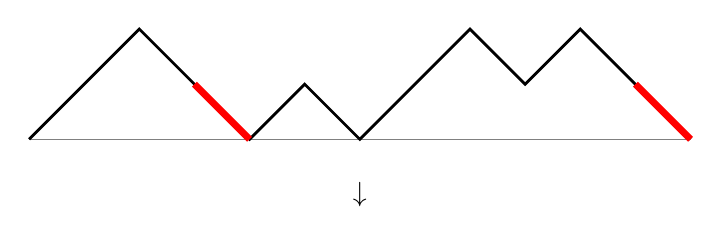
\begin{tikzpicture}[scale=.7]
\draw[help lines] (0,0) grid (12,0);
\draw[line width = 1pt] (0,0) -- ++(1,1) -- ++(1,1) -- ++(1,-1) -- ++(1,-1) -- ++(1,1) -- ++(1,-1) -- ++(1,1) -- ++(1,1) -- ++(1,-1) -- ++(1,1) -- ++(1,-1) -- ++(1,-1);
  \node at (6,-1) {\( \downarrow \)};
\draw[line width = 2.5pt,red] (3,1) -- (4,0);
\draw[line width = 2.5pt,red] (11,1) -- (12,0);
\end{tikzpicture}

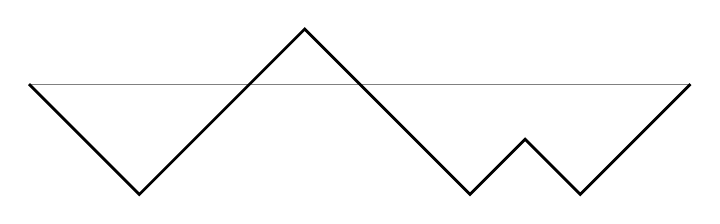
\begin{tikzpicture}[scale=.7]
\draw[help lines] (0,0) grid (12,0);
\draw[line width = 1pt] (0,0) -- ++(1,-1) -- ++(1,-1) -- ++(1,1) -- ++(1,1) -- ++(1,1) -- ++(1,-1) -- ++(1,-1) -- ++(1,-1) -- ++(1,1) -- ++(1,-1) -- ++(1,1) -- ++(1,1);
\end{tikzpicture}
      \caption{The map reflecting each path with a red down step.}
      \label{fig:reflect}
    \end{figure}


    This map gives a bijection between the colored Dyck paths from
    \( (0,0) \) to \( (2n,0) \) to any path from \( (0,0) \) to
    \( (2n,0) \) consisting of up steps and down steps. Since there
    are \( \binom{2n}{n} \) such paths, we obtain the result.
  \end{proof}
  

\section{Hermite polynomials}

The \emph{Hermite polynomials} \( H_n(x) \) are defined by
\( H_{-1}(x) = 0 \), \( H_{0}(x) = 1 \), and
\[
  H_{n+1}(x) = 2x H_n(x) - 2n H_{n-1}(x), \qquad  n\ge1.
\]
Since the leading coefficient of \( H_n(x) \) is \( 2^n \), we can
make it monic by letting \( \hat{H}_n(x) = 2^{-n}H_n(x) \). Then
\( \hat{H}_{-1}(x) = 0 \), \( \hat{H}_{0}(x) = 1 \), and
\begin{equation}\label{eq:25}
  \hat{H}_{n+1}(x) = x \hat{H}_n(x) - \frac{n}{2} \hat{H}_{n-1}(x), \qquad  n\ge1.
\end{equation}

For the combinatorial study of orthogonal polynomials, it is more
convenient if the recurrence coefficients \( b_n \) and
\( \lambda_n \) are integers. We can rescale orthogonal polynomials
using the following lemma.

\begin{lem}[Rescaling OPS] \label{lem:rescaling} 
  Suppose that \( \{ P_n(x) \}_{n\ge 0} \) is a monic OPS such that
  \( P_{-1}(x) = 0 \), \( P_{0}(x) = 1 \), and
  \begin{equation}\label{eq:23}
      P_{n+1}(x) = (x-b_n) P_n(x) - \lambda_n P_{n-1}(x), \qquad n\ge1.
  \end{equation}
  Let \( \widetilde{P}_n(x) = a^n P_n(x/a) \), where \( a\ne0 \). Then
  \( \widetilde{P}_{-1}(x) = 0 \), \( \widetilde{P}_{0}(x) = 1 \), and
  \begin{equation}\label{eq:24}
    \widetilde{P}_{n+1}(x) = (x-ab_n) \widetilde{P}_n(x) - a^2\lambda_n
    \widetilde{P}_{n-1}(x), \qquad n\ge1.
  \end{equation}
\end{lem}
\begin{proof}
  Replacing \( x \) by \( x/a \) and multiplying both sides by
  \( a^{n+1} \) in \eqref{eq:23} yields \eqref{eq:24}.
\end{proof}

Define the \emph{rescaled Hermite polynomials}
\( \widetilde{H}_n(x) \) by
\( \widetilde{H}_n(x) = \sqrt{2}^n \hat{H}_n(x/\sqrt{2}) \). By
\Cref{lem:rescaling} and \eqref{eq:25},
\( \widetilde{H}_{-1}(x) = 0 \), \( \widetilde{H}_1(x) = 1 \), and 
\begin{equation}\label{eq:hermite-3rr}
  \widetilde{H}_{n+1}(x) = x \widetilde{H}_n(x) - n
  \widetilde{H}_{n-1}(x), \qquad n\ge1.
\end{equation}

We note that \( H_n(x) \) are called ``physicist's Hermite
polynomials'' and \( \widetilde{H}_n(x) \) are called ``probabilist's
Hermite polynomials''.

The moment \( \mu_n \) of \( \{ \widetilde{H}_n(x) \}_{n\ge 0} \) 
is given by
\[
  \mu_n = \sum_{\pi\in\Motz_n} \wt(\pi),
\]
where \( \wt(\pi) \) is determined by \( b_n=0 \) and
\( \lambda_n=n \). Since \( b_n=0 \),
we have \( \mu_{2n+1}=0 \) and
\[
  \mu_{2n} = \sum_{\pi\in\Dyck_{2n}} \wt(\pi).
\]
Note that for each \( \pi\in\Dyck_{2n} \), its weight \( \wt(\pi) \)
is a positive integer. It is thus natural to ask what combinatorial
objects \( \wt(\pi) \) counts.

\begin{defn}
  A \emph{Hermite history} is a Dyck path where each down step
  starting at height \( k \) has a label in \( \{0,1,\dots,k-1\} \).
  Let \( \HH_{2n} \) denote the set of Hermite histories whose
  underlying Dyck paths are from \( (0,0) \) to \( (2n,0) \).
\end{defn}

Let \( \pi\in\Dyck_{2n} \). For each down step of \( \pi \) starting
at height \( k \), there are \( k \) ways to assign a label from
\( \{0,1,\dots,k-1\} \). Thus \( \wt(\pi) \) is the number of Hermite
histories with underlying Dyck path \( \pi \). This implies
\( \mu_{2n} = |\HH_{2n}|  \).

Let \( \CM_{2n} \) be the set of complete matchings on \( [2n] \).

\begin{prop}
  There is a bijection between \( \HH_{2n} \) and \( \CM_{2n} \).
\end{prop}

\begin{proof}
  Let \( \pi\in \HH_{2n} \). We construct a complete matching
  \( \rho \) as follows. For \( k= 1,\dots,2n \), if the \( k \)th
  step of \( \pi \) is an up step, then make the \( k \)th vertex of
  \( \rho \) to be an \emph{opener}, which means it will be connected
  to a vertex to its right. If the \( k \)th step of \( \pi \) is a
  down step, then make the \( k \)th vertex of \( \rho \) to be a
  \emph{closer}, which means it will be connected to a vertex to its
  left. If the \( k \)th step of \( \pi \) is a down step with label
  \( a_k \), then connected the vertex at \( k \) with the closest
  available opener skipping \( a_k \) openers. For example, see
  \Cref{fig:Hermite-history}.

  Observe that the height of the starting point of the \( k \)th down
  step is equal to the number of available openers for the vertex
  \( k \). Therefore the map \( \pi\mapsto \rho \) is well-defined.
  The inverse map \( \rho\mapsto \pi \) is straighforward to
  construct. Hence the map \( \pi\mapsto \rho \) is a bijection from
  \( \HH_{2n} \) and \( \CM_{2n} \).
\end{proof}

\begin{figure}
  \centering
 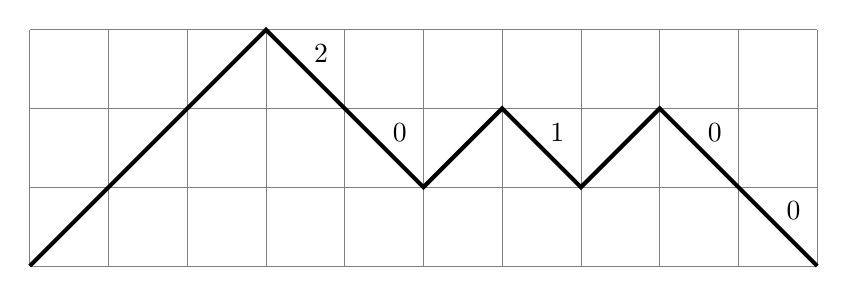
\begin{tikzpicture}
\draw[help lines] (0,0) grid (10,3);
\draw[line width = 1.5pt] (0,0) -- ++(1,1) -- ++(1,1) -- ++(1,1) -- ++(1,-1) -- ++(1,-1) -- ++(1,1) -- ++(1,-1) -- ++(1,1) -- ++(1,-1) -- ++(1,-1);
\node at (3.7,2.7) {2};
\node at (4.7,1.7) {0};
\node at (6.7,1.7) {1};
\node at (8.7,1.7) {0};
\node at (9.7,0.7) {0};
\end{tikzpicture}

\begin{tikzpicture}
\begin{scope}[shift={(0,0)}]
\node (0,0) at (1,1) {};
\draw (1,0) -- (1.3,0.3);
\draw (2,0) -- (2.3,0.3);
\draw (3,0) -- (3.3,0.3);
\draw (4,0) -- (3.7,0.3);
\draw (5,0) -- (4.7,0.3);
\draw (6,0) -- (6.3,0.3);
\draw (7,0) -- (6.7,0.3);
\draw (8,0) -- (8.3,0.3);
\draw (9,0) -- (8.7,0.3);
\draw (10,0) -- (9.7,0.3);
\node[draw,circle,fill=white] (1) at (1,0) {};
\node[draw,circle,fill=white] (4) at (4,0) {};
\node[draw,circle,fill=white] (2) at (2,0) {};
\node[draw,circle,fill=white] (7) at (7,0) {};
\node[draw,circle,fill=white] (3) at (3,0) {};
\node[draw,circle,fill=white] (5) at (5,0) {};
\node[draw,circle,fill=white] (6) at (6,0) {};
\node[draw,circle,fill=white] (10) at (10,0) {};
\node[draw,circle,fill=white] (8) at (8,0) {};
\node[draw,circle,fill=white] (9) at (9,0) {};
\end{scope}
\end{tikzpicture}

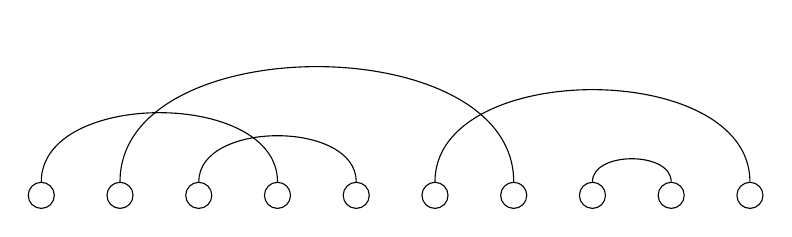
\begin{tikzpicture}
\begin{scope}[shift={(0,0)}]
\node (0.5) at (1,0) {};
\node[draw, circle] (1) at (1,0) {};
\node[draw, circle] (4) at (4,0) {};
\draw[out=90,in=90] (1) to (4);
\node[draw, circle] (2) at (2,0) {};
\node[draw, circle] (7) at (7,0) {};
\draw[out=90,in=90] (2) to (7);
\node[draw, circle] (3) at (3,0) {};
\node[draw, circle] (5) at (5,0) {};
\draw[out=90,in=90] (3) to (5);
\node[draw, circle] (6) at (6,0) {};
\node[draw, circle] (10) at (10,0) {};
\draw[out=90,in=90] (6) to (10);
\node[draw, circle] (8) at (8,0) {};
\node[draw, circle] (9) at (9,0) {};
\draw[out=90,in=90] (8) to (9);
\end{scope}
\end{tikzpicture}
\caption{A Hermite history (top), the openers and closers (middle),
  and the corresponding matching (bottom).}
  \label{fig:Hermite-history}
\end{figure}

Since the number of complete matchings on \( [2n] \) is
\( (2n-1)!! \), we obtain the following result.

\begin{cor}
  The \( 2n \)th moment of rescaled Hermite polynomials
  \( \widetilde{H}_n(x) \) is
  \[
    \mu_{2n} = (2n-1)!!.
  \]
\end{cor}


\section{Charlier polynomials}

The (normalized) \emph{Charlier polynomials}
\( C_n(x;a) \) are defined by
\( C_{-1}(x;a) =0 \), \( C_{1}(x;a) =1 \), and
\[
  C_{n+1}(x;a) = (x-n-a) C_n(x;a) - an C_{n-1}(x;a), \qquad n\ge1.
\]

\begin{defn}
  A \emph{Charlier history} is a Motzkin path where each horizontal
  step at height \( k \) has a label in \( \{0,1,\dots,k\} \) and each
  down step starting at height \( k \) has a label in
  \( \{0,1,\dots,k-1\} \). Let \( \CH_{n} \) denote the set of
  Charlier histories whose underlying Motzkin paths are from
  \( (0,0) \) to \( (n,0) \).
  For \( \pi\in \CH_{n} \), define the weight \( \wt(\pi) \)
  to be the product of the weights of its steps, where
  \begin{itemize}
  \item the weight of an upstep is \( 1 \),
  \item the weight of a horizontal step of height \( k \) is \( 1 \)
    if its label is less than \( k \) and \( \alpha \) if its label is
    \( k \),
  \item the weight of a down step is \( \alpha \).
  \end{itemize}
\end{defn}

By the definition of the Charlier histories, the moment \( \mu_n \) of
the Charlier polynomials is given by
\[
  \mu_n = \sum_{\pi\in \Motz_n} \wt(\pi) = \sum_{\pi\in \CH_n}
  \wt(\pi).
\]

For a set partition \( \sigma \), let \( \block(\sigma) \) denote the
number of blocks in \( \sigma \).

\begin{thm}
  The moment \( \mu_n \) of the Charlier polynomials is given by
\[
  \mu_n = \sum_{\sigma\in \Pi_n} \alpha^{\block(\sigma)}.
\]
\end{thm}

\begin{proof}
  We will construct a weight-preserving bijection
  \( \phi:\CH_n\to \Pi_n \). Let \( \pi\in \CH_n \). We construct the
  corresponding set partition \( \phi(\pi) = \sigma\in\Pi_n \) as
  follows. For \( k= 1,\dots,n \),
\begin{itemize}
\item if the \( k \)th step of \( \pi \) is an up step, then make the
  \( k \)th vertex of \( \sigma \) to be an opener,
\item if the \( k \)th step of \( \pi \) is a down step, then make
  the \( k \)th vertex of \( \rho \) to be a closer,
\item if the \( k \)th step of \( \pi \) is a horizontal step, then
  make the \( k \)th vertex of \( \rho \) to be a \emph{transient},
  which means that it is connected to a vertex to its left and also a
  vertex to its right.
\end{itemize}
If the \( k \)th step of \( \pi \) is a down step with label
\( a_k \), then connected the vertex at \( k \) with the closest
available opener or transient skipping \( a_k \) of them. If the
\( k \)th step of \( \pi \) is a horizontal step with label \( a_k \),
then connected the vertex at \( k \) with the closest available opener
or transient skipping \( a_k \) of them. Here, if \( a_k \) is equal
to the height of the horizontal step, ``skipping all available openers
and transients'' means the vertex \( k \) is connected to itself
making it a singleton. For example, see \Cref{fig:Charlier-history}.

  Observe that the height of the starting point of the \( k \)th down
  step is equal to the number of available openers for the vertex
  \( k \). Therefore the map \( \pi\mapsto \rho \) is well-defined.
  The inverse map \( \rho\mapsto \pi \) is straighforward to
  construct. Hence the map \( \pi\mapsto \rho \) is a bijection from
  \( \HH_{2n} \) and \( \CM_{2n} \).

  It is not hard to see that \( \phi:\CH_n\to \Pi_n \) is a bijection.
  Moreover, if \( \phi(\pi) = \rho \), then
  \( \wt(\pi) = \alpha^{a+b} = \alpha^{\block(\rho)} \), where \( a \)
  is the number of horizontal steps with maximum label and \( b \) is
  the number of down steps in \( \pi \). This can be seen from the
  observation that every block of \( \rho \) is either a singleton
  (corresponding to a horizontal step of maximum label) or a block
  with exactly one closer (corresponding to a down step). This
  completes the proof.
\end{proof}

\begin{figure}
  \centering
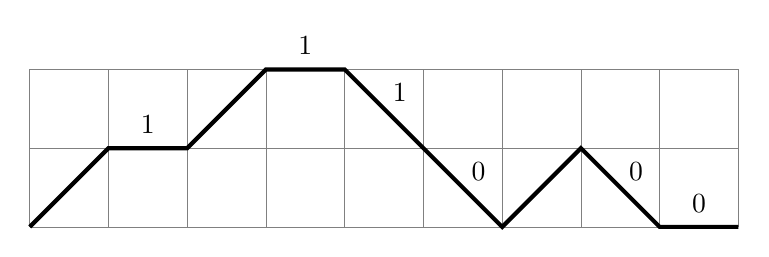
\begin{tikzpicture}
\draw[help lines] (0,0) grid (9,2);
\draw[line width = 1.5pt] (0,0) -- ++(1,1) -- ++(1,0) -- ++(1,1) -- ++(1,0) -- ++(1,-1) -- ++(1,-1) -- ++(1,1) -- ++(1,-1) -- ++(1,0);
\node at (4.7,1.7) {1};
\node at (5.7,0.7) {0};
\node at (7.7,0.7) {0};
\node at (8.5,0.3) {0};
\node at (1.5,1.3) {1};
\node at (3.5,2.3) {1};
\end{tikzpicture}
 
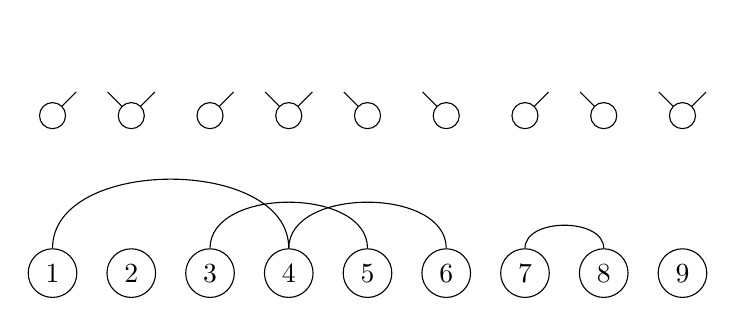
\begin{tikzpicture}
\begin{scope}[shift={(0,0)}]
\node (0,0) at (1,1) {};
\draw (1,0) -- (1.3,0.3);
\draw (1.7,0.3) -- (2,0) -- (2.3,0.3);
\draw (3,0) -- (3.3,0.3);
\draw (3.7,0.3) -- (4,0) -- (4.3,0.3);
\draw (5,0) -- (4.7,0.3);
\draw (6,0) -- (5.7,0.3);
\draw (7,0) -- (7.3,0.3);
\draw (8,0) -- (7.7,0.3);
\draw (8.7,0.3) -- (9,0) -- (9.3,0.3);
\node[draw,circle,fill=white] (1) at (1,0) {};
\node[draw,circle,fill=white] (4) at (4,0) {};
\node[draw,circle,fill=white] (2) at (2,0) {};
\node[draw,circle,fill=white] (7) at (7,0) {};
\node[draw,circle,fill=white] (3) at (3,0) {};
\node[draw,circle,fill=white] (5) at (5,0) {};
\node[draw,circle,fill=white] (6) at (6,0) {};
\node[draw,circle,fill=white] (8) at (8,0) {};
\node[draw,circle,fill=white] (9) at (9,0) {};
\end{scope}
\begin{scope}[shift={(0,-2)}]
\node[draw, circle] (1) at (1,0) {\( 1 \)};
\node[draw, circle] (4) at (4,0) {\( 4 \)};
\node[draw, circle] (6) at (6,0) {\( 6 \)};
\draw[out=90,in=90] (1) to (4);
\draw[out=90,in=90] (4) to (6);
\node[draw, circle] (2) at (2,0) {\( 2 \)};
\node[draw, circle] (3) at (3,0) {\( 3 \)};
\node[draw, circle] (5) at (5,0) {\( 5 \)};
\draw[out=90,in=90] (3) to (5);
\node[draw, circle] (7) at (7,0) {\( 7 \)};
\node[draw, circle] (8) at (8,0) {\( 8 \)};
\draw[out=90,in=90] (7) to (8);
\node[draw, circle] (9) at (9,0) {\( 9 \)};
\end{scope}
\end{tikzpicture}

\caption{A Charlier history (top), the openers, closers, and
  transients (middle), and the corresponding set partition (bottom).}
  \label{fig:Charlier-history}
\end{figure}


\section{Laguerre polynomials}

The (normalized) \emph{Laguerre polynomials}
\( L^{(\alpha)}_n(x) \) are defined by
\( L^{(\alpha)}_{-1}(x) =0 \), \( L^{(\alpha)}_{1}(x) =1 \), and
\[
  L^{(\alpha)}_{n+1}(x) = (x-2n-\alpha) L^{(\alpha)}_n(x) - n(n-1+\alpha) L^{(\alpha)}_{n-1}(x), \qquad n\ge1.
\]


\begin{lem}
  Suppose that \( \{ P_n(x) \}_{n\ge 0} \) is a monic OPS such that
  \[
    P_{n+1}(x) = (x-b_n) P_n(x) - a_nc_n P_{n-1}(x).
  \]
  Then
  \[
    \mu_n = \sum_{\pi\in \Motz_n} \wt'(\pi),
  \]
  where \( \wt'(\pi) \) is the product of the weights of the steps in \( \pi \) and
  \begin{itemize}
  \item the weight of an up step ending at height \( k \) is \( a_k \),
  \item the weight of a horizontal step at height \( k \) is \( b_k \),
  \item the weight of a down step starting at height \( k \) is \( c_k \).
  \end{itemize}
\end{lem}

\begin{proof}
  We know that
  \[
    \mu_n = \sum_{\pi\in \Motz_n} \wt(\pi),
  \]
  where \( \wt(\pi) \) is the product of \( b_k \) for each horizontal
  step of height \( k \) and \( \lambda_k = a_kc_k \) for each down
  step starting at height \( k \). Observe that for
  \( \pi\in \Motz_n \) every down step corresponds to a unique up
  step. Thus we can split the weight \( \lambda_k=a_kc_k \) on a down
  step starting at height \( k \) into the weight \( a_k \) of the
  corresponding up step and the weight \( c_k \) of the down step as
  shown in \Cref{fig:up-down}. This proves the lemma.
  \begin{figure}
    \centering
    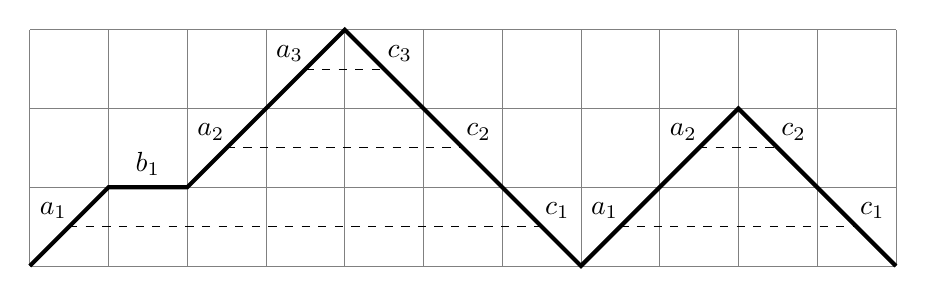
\begin{tikzpicture}
\draw[help lines] (0,0) grid (11,3);
\draw[line width = 1.5pt] (0,0) -- ++(1,1) -- ++(1,0) -- ++(1,1) -- ++(1,1) -- ++(1,-1) -- ++(1,-1) -- ++(1,-1) -- ++(1,1) -- ++(1,1) -- ++(1,-1) -- ++(1,-1);
\draw[dashed] (0.5,0.5) -- (6.5,0.5);
\draw[dashed] (2.5,1.5) -- (5.5,1.5);
\draw[dashed] (3.5,2.5) -- (4.5,2.5);
\draw[dashed] (7.5,0.5) -- (10.5,0.5);
\draw[dashed] (8.5,1.5) -- (9.5,1.5);
\node at (0.3,0.7) {\( a_1 \)};
\node at (1.5,1.3) {\( b_1 \)};
\node at (2.3,1.7) {\( a_2 \)};
\node at (3.3,2.7) {\( a_3 \)};
\node at (4.7,2.7) {\( c_3 \)};
\node at (5.7,1.7) {\( c_2 \)};
\node at (6.7,0.7) {\( c_1 \)};
\node at (7.3,0.7) {\( a_1 \)};
\node at (8.3,1.7) {\( a_2 \)};
\node at (9.7,1.7) {\( c_2 \)};
\node at (10.7,0.7) {\( c_1 \)};
\end{tikzpicture}
\caption{Splitting the weight \( \lambda_k=a_kc_k \)
  into \( a_k \) and \( c_k \).}
    \label{fig:up-down}
  \end{figure}
\end{proof}

\begin{defn}
  A \emph{Laguerre history} is a Motzkin path where 
\begin{itemize}
\item each up step starting at height \( k \)
  has a label in \( \{0,1,\dots,k\} \),
\item each horizontal step at height \( k \) has a label in
  \( \{-k,\dots,-1,0,1,\dots,k\} \),
\item  each down step starting at height \( k \)
  has a label in \( \{1,2,\dots,k\} \),
\end{itemize}

 Let \( \LH_{n} \) denote the set of
  Laguerre histories whose underlying Motzkin paths are from
  \( (0,0) \) to \( (n,0) \).
  For \( \pi\in \LH_{n} \), define the weight \( \wt(\pi) \)
  to be the product of the weights of its steps, where
  \begin{itemize}
  \item the weight of an upstep is \( 1 \) if its label is nonzero
    and \( \alpha \) if its label is \( 0 \),
  \item the weight of a horizontal step of height \( k \) is \( 1 \)
    if its label is nonzero and \( \alpha \) if its label is \( 0 \),
  \item the weight of a down step is \( \alpha \).
  \end{itemize}
\end{defn}

We have
\[
  \mu_n = \sum_{\pi\in \LH_n} \wt(\pi).
\]

\begin{thm}
\[
  \mu_n = \sum_{\pi\in \sym_n} \alpha^{\cycle(\pi)}.
\]
\end{thm}

There are several bijections between \( \sym_n \) and \( \LH_n \) due
to Fran\c{c}on--Viennot \cite{Francon1979}, Foata--Zeilberger
\cite{Foata1990a}, see also \cite[Algorithm~7]{Corteel2020a}.

We will use a slight modification of the bijection due to
Fran\c{c}on--Viennot \cite{Francon1979}.

Let \( \pi \in \LH_n \).
Let \( S_k \) be the \( k \)th step of \( \pi \)
and let \( \ell_k \) be its label.

For each \( k= 0,1,\dots,n \), we will construct a list \( A_k \) of
cycles of integers and dots, \( \fcirc \)'s. First we set
\( A_0 = \emptyset \). We then construct \( A_{k} \) recursively as follows.
\begin{description}
\item[Case 1:] \( S_k \) is an up step.
  \begin{description}
  \item[Case 1-1:] \( \ell_k=0 \). Create a new
  cycle \( (k\fcirc) \) at the beginning:
  \[
    A_k = (k\fcirc) A_{k-1}.
  \]
\item[Case 1-2:] \( \ell_k=i>0 \). Replace the
  \( i \)th dot in \( A_{k-1} \) by ``\( \fcirc k \fcirc \)''.
  \end{description}
\item[Case 2:] \( S_k \) is a horizontal step.
  \begin{description}
  \item[Case 2-1:] \( \ell_k=0 \). Create a new cycle \( (k) \) at the
    beginning:
  \[
    A_k = (k) A_{k-1}.
  \]
\item[Case 2-2:] \( \ell_k=i>0 \). Replace the \( i \)th dot in
  \( A_{k-1} \) by ``\( k \fcirc \)''.
\item[Case 2-3:] \( \ell_k=-i<0 \). Replace the \( i \)th dot in
  \( A_{k-1} \) by ``\( \fcirc k \)''.
  \end{description}

\item[Case 3:] \( S_k \) is a down step. Then \( \ell_k=i>0 \).
  Replace the \( i \)th dot in \( A_{k-1} \) by ``\( k \)''.
\end{description}

The number of dots in \( A_{k} \) is always equal to the height of
\( S_1 \cdots S_k \). Therefore the above construction is well
defined.


\chapter{Mixed moments and coefficients}

Let
\begin{align*}
  x^n &= \sum_{k=0}^{n} \mu_{n,k} P_k(x),\\
  P_n(x) &= \sum_{k=0}^{n} \nu_{n,k} x^k.
\end{align*}
Then
\[
  \left( \mu_{n,k} \right)_{n,k\ge0} \left( \nu_{n,k} \right)_{n,k\ge0} = 
  \left( \nu_{n,k} \right)_{n,k\ge0} \left( \mu_{n,k} \right)_{n,k\ge0} = I.
\]

Since we have combinatorial interpretations for \( \mu_{n,k} \) and
\( \nu_{n,k} \), we can prove the above matrix identities
combinatorially.

In fact, we will prove these without the assumption that
\( \lambda_k\ne 0 \).


% \chapter{Determinants of moments}

% \section{Computing the 3-term recurrence coefficients}

% \section{The Lindstr\"om--Gessel--Viennot lemma}

% \section{Hankel determinants of moments}

% \section{The duality between Motzkin paths and Favard paths}

% \section{Inverse generating functions}

% \chapter{Continued fractions}

% \section{Development in J-fraction}

% \section{Examples}

% \section{Convergents}

% \section{Symmetric orthogonal polynomials}

% \chapter{Linearization coefficients}



\newpage

\appendix

\chapter{Sign-reversing involutions}
\label{sec:sign-revers-invol}

\begin{defn}
  A \emph{sign} of a set \( X \) is a function
  \( \sgn:X \to \{+1,-1\} \). A \emph{sign-reversing involution} on
  \( X \) is an involution \( \phi:X\to X \) such that
  \begin{enumerate}
  \item \( \sgn(x)=1 \) for all \( x\in \Fix(\phi) \);
  \item \( \sgn(\phi(x)) = -\sgn(x) \) for all
  \( x\in X \setminus \Fix(\phi) \),
  \end{enumerate}
  where \( \Fix(\phi) \) is the set of \emph{fixed points} of
  \( \phi \), i.e., \( \Fix(\phi) = \{x\in X: \phi(x) = x \} \).
\end{defn}

It is easy to see that if \( \phi \) is a sign-reversing involution on
\( X \), then
\begin{equation}\label{eq:sgnsum=Fix}
  \sum_{x\in X} \sgn(X) = |\Fix(\phi)|.
\end{equation}

\begin{exam}
  Let's prove the following identity using sign-reversing involutions:
  \begin{equation}\label{eq:4}
    \sum_{k=0}^{n} (-1)^{k} \binom{n}{k} = 0.
  \end{equation}
  To this end we need to construct a set \( X \) and a sign-reversing
  involution \( \phi \) on \( X \) such that \eqref{eq:sgnsum=Fix}
  becomes \eqref{eq:4}.

  Let \( X \) be the set of all subsets of \( [n]:= \{ 1,\dots,n \} \)
  and for \( A\in X \), define \( \sgn(A) = (-1)^{|A|} \). Then it
  suffices to construct a sign-reversing involution on \( X \) with no
  fixed points. This can be done by letting
  \( \phi(A) = A \Delta \{1\} \), where
  \( A \Delta B := (A \cup B) \setminus (A \cap B) \).
\end{exam}


\begin{exam}
  Recall that we proved the following identitiy, which was stated in
  \eqref{eq:charlier-orthogonality}, using generating functions:
  \begin{equation}\label{eq:charlier-orthogonality2}
  \sum_{k\ge 0}  P_m(k) P_n(k) \frac{a^k}{k!} = \frac{e^a a^n}{n!} \delta_{n,m},
  \end{equation}
  where \( P_n(x) \) are the Charlier polynomials defined by
  \[
    P_n(x) = \sum_{k=0}^{n} \binom{x}{k} \frac{(-a)^{n-k}}{(n-k)!}.
  \]
  We will prove this identity using sign-reversing involutions. To do
  this, we will consider \eqref{eq:charlier-orthogonality2} as a power
  series in \( a \). Note that
\begin{align*}
  \sum_{k\ge 0}  P_m(k) P_n(k) \frac{a^k}{k!}
  &=  \sum_{k\ge 0} \sum_{i=0}^m \binom{k}{i} \frac{(-a)^{m-i}}{(m-i)!}
  \sum_{j=0}^n \binom{k}{j} \frac{(-a)^{n-j}}{(n-j)!} \frac{a^k}{k!}\\
  &=  \sum_{k\ge 0} \sum_{i=0}^m \sum_{j=0}^n
    \binom{k}{m-i} \frac{(-a)^{i}}{i!}
   \binom{k}{n-j} \frac{(-a)^{j}}{j!} \frac{a^k}{k!}\\
  &= \sum_{N\ge0} \frac{a^N}{N!} \sum_{i+j+k=N}
  (-1)^{i+j} \frac{N!}{i!j!k!} \binom{k}{m-i} \binom{k}{n-j},
\end{align*}
where \( \binom{r}{s}=0 \) if \( s<0 \).

For a fixed \( N \),
\[
  \sum_{i+j+k=N} (-1)^{i+j} \binom{N}{i,j,k} \binom{k}{m-i} \binom{k}{n-j}
  = \sum_{(A,B,C)\in X} (-1)^{|B\setminus A| + |C\setminus A|},
\]
where \( X \) is the set of triples \( (A,B,C) \) such that
\( A\cup B\cup C = \{ 1,\dots,N \} \), \( |A|=k, |B|=m, |C|=n \),
\( (B\cap C)\setminus A = \emptyset \). Define
\( \sgn(A,B,C) = (-1)^{|B\setminus A| + |C\setminus A|} \). We will
find a sign-reversing involution on \( X \) toggling the smallest
integer in regions \( 1 \) and \( 2 \) or in regions \( 3 \) and
\( 4 \) in Figure~\ref{fig:image1}.
\begin{figure}
  \centering
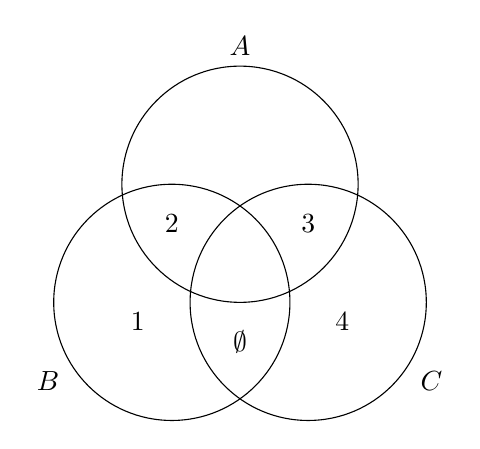
\begin{tikzpicture}
\node [draw, circle, minimum size =3cm,
    label={90:$A$}] (A) at (90:1){};
\node [draw, circle, minimum size =3cm,
    label={210:$B$}] (B) at (210:1){};
\node [draw, circle, minimum size =3cm,
    label={330:$C$}] (C) at (330:1){};
\node at (270:1) {\( \emptyset \)};
\node at (150:1) {\( 2 \)};
\node at (30:1) {\( 3 \)};
\node at (210:1.5) {\( 1 \)};
\node at (330:1.5) {\( 4 \)};
\end{tikzpicture}
  \caption{The triple \( (A,B,C) \).}
  \label{fig:image1}
\end{figure}

To be precise, for \( (A,B,C)\in X \), define \( \phi(A,B,C) \) as
follows.
\begin{description}
\item[Case 1] The regions \( 1,2,3,4 \) are all empty. In this case we define
  \( \phi(A,B,C) = (A,B,C) \).
\item[Case 2] At least one of the regions \( 1,2,3,4 \) is nonempty.
  Let \( s \) be the smallest integer in \( (B\cap C) \setminus A \).
  If \( s \) is in region \( 1 \) (respectively 2, 3, 4), then move
  this integer to region \( 2 \) (respectively 1, 4, 3). Then let
  \( \phi(A,B,C) = (A',B',C') \), where \( A',B',C' \) are the
  resulting sets.
\end{description}

By the construction, \( \phi \) is a sign-reversing involution on
\( X \) whose fixed points are the triples \( (A,B,C) \) such that the
regions \( 1,2,3,4 \) are all empty, that is, \( B=C \subseteq A \).
If \( B=C \subseteq A \), then \( A = [N] \),
so the number of such triples \( (A,B,C) \) is
\( \binom{N}{n} \) if \( m=n \)
and \( 0 \) otherwise.
Thus
\[
  \sum_{(A,B,C)\in X} (-1)^{|B\setminus A| + |C\setminus A|} =
  |\Fix(\phi)| = \delta_{m,n} \binom{N}{n}.
\]
This implies
\[
  \sum_{k\ge 0}  P_m(k) P_n(k) \frac{a^k}{k!}
  = \delta_{m,n} \sum_{N\ge0} \frac{a^N}{N!} \binom{N}{n}
  = \frac{e^a a^n}{n!} \delta_{n,m}.
\]
\end{exam}






\bibliographystyle{abbrv}
\bibliography{/Users/jangsookim/Library/CloudStorage/Dropbox/newbiemacs/nbm-user-settings/references/ref.bib}

\end{document}
